% !TEX TS-program = pdflatex
% !TEX encoding = UTF-8 Unicode

% This is a simple template for a LaTeX document using the "article" class.
% See "book", "report", "letter" for other types of document.

\documentclass[11pt]{article} % use larger type; default would be 10pt

\usepackage[utf8]{inputenc} % set input encoding (not needed with XeLaTeX)
\usepackage{tikz}
%%% Examples of Article customizations
% These packages are optional, depending whether you want the features they provide.
% See the LaTeX Companion or other references for full information.

%%% PAGE DIMENSIONS
\usepackage{geometry} % to change the page dimensions
\geometry{a4paper} % or letterpaper (US) or a5paper or....
% \geometry{margins=2in} % for example, change the margins to 2 inches all round
% \geometry{landscape} % set up the page for landscape
%   read geometry.pdf for detailed page layout information

\usepackage{graphicx} % support the \includegraphics command and options

% \usepackage[parfill]{parskip} % Activate to begin paragraphs with an empty line rather than an indent

%%% PACKAGES
\usepackage{booktabs} % for much better looking tables
\usepackage{array} % for better arrays (eg matrices) in maths
\usepackage{paralist} % very flexible & customisable lists (eg. enumerate/itemize, etc.)
\usepackage{verbatim} % adds environment for commenting out blocks of text & for better verbatim
\usepackage{subfig} % make it possible to include more than one captioned figure/table in a single float
% These packages are all incorporated in the memoir class to one degree or another...
\usepackage{url}
\usepackage{hyperref}

%%% HEADERS & FOOTERS
\usepackage{fancyhdr} % This should be set AFTER setting up the page geometry
\pagestyle{fancy} % options: empty , plain , fancy
\renewcommand{\headrulewidth}{0pt} % customise the layout...
\lhead{}\chead{}\rhead{}
\lfoot{}\cfoot{\thepage}\rfoot{}

%%% SECTION TITLE APPEARANCE
\usepackage{sectsty}
\allsectionsfont{\sffamily\mdseries\upshape} % (See the fntguide.pdf for font help)
% (This matches ConTeXt defaults)

%%% ToC (table of contents) APPEARANCE
\usepackage[nottoc,notlof,notlot]{tocbibind} % Put the bibliography in the ToC
\usepackage[titles,subfigure]{tocloft} % Alter the style of the Table of Contents
\renewcommand{\cftsecfont}{\rmfamily\mdseries\upshape}
\renewcommand{\cftsecpagefont}{\rmfamily\mdseries\upshape} % No bold!

%%% END Article customizations

%%% The "real" document content comes below...

\usepackage{amsfonts}
\usepackage{amsmath}
\usepackage{amsthm}
\usepackage{amssymb}
\usepackage{qtree}

\theoremstyle{definition}
\newtheorem*{beispiel}{Beispiel}
\newtheorem{definition}{Definition}
\newtheorem*{bemerkung}{Bemerkung}
\newtheorem*{beweis}{Beweis}
\newtheorem*{ubung}{Übung}
\newtheorem{theorem}{Theorem}

\title{Theoretische Informatik -- Schreibomat}
\author{Florian}
%\date{} % Activate to display a given date or no date (if empty),
         % otherwise the current date is printed 

\begin{document}
\maketitle

\section*{Tools}
\begin{itemize}
\item Finite State Machine Designer: \url{http://madebyevan.com/fsm/}
\end{itemize}

\section{Was ist Informatik?}

\begin{itemize}

\item Konkrete\footnote{4. September 2012} Konzepte: Algorithmus, Berechnung, Komplexität

\item Was will die theoretische Informatik? Formale Bestimmung der Begriffe, unabhängig von Hard- und Software

\item Ziel: Grundlegende Eigenschaften von Algorithmen, Berechnungen erkennen. Methoden entwickeln zum Entwurf beweisbar korrekter Hard- und Software (nicht Schwerpunkt dieser Vorlesung)

\item Grenzen der automatischen Berechnung aufzeigen

\item Typische Fragestellungen: Ist es möglich, ein Programm zu schreiben, das ein anderes Programm als Eingabe erhält und feststellen kann, ob dieses in eine Endlosschleife gerät oder nicht? $\Rightarrow$ Halteproblem. Nein, es ist natürlich nicht möglich. Eine andere typische Fragestellung ist die Folgende: Wir haben einen Rucksack, und der hat 30 Liter Fassungsvermögen. Und wir haben noch 50 Gegenstände, und jetzt wollen wir wissen: wie lange dauert es, herauszufinden, wieviele Gegenstände in den Rucksack passen? Rucksackproblem, nicht in polynomialer Zeit lösbar $\Rightarrow$ Es dauert expontiell lange.

\item Leider ist es in der Praxis so, dass die Antwort auf ähnliche Fragestellungen nicht immer so offensichtlich ist, und deshalt müssen wir es uns ein bisschen genauer betrachten.

\end{itemize}

\begin{ubung}

Gegeben sei das folgende Strassennetz:

(Wildes Gekritzel)

\begin{enumerate}[(a)]
\item Gibt es eine Möglichkeit, alle Strassen genau 1x zu durchlaufen und dann wieder am Ausgangspunkt anzulangen,
\item Gibt es eine Möglichkeit, alle Kreuzungen genau 1x zu passieren und dann wieder am Ausgangspunkt anzulangen?
\end{enumerate}

Die Antworten sind imfall:
\begin{enumerate}[(a)]
\item Einfache Aufgabe: Geht immer, wenn die Anzahl der Abzweigungen an jeder Kreuzung gerade ist.
\item Traveling salesman (TSP). Schwierig! Es ist keine wesentlich bessere Methode bekannt, als einfach alles durchzuprobieren.
\end{enumerate}

\end{ubung}

Ziel für die Vorlesung: Um solche Fragestellungen systematisch beantworten zu können, brauchen wir ein exaktes mathematisches Modell eines Computers.

\section{Automatentheorie}

Endliche Automaten, Kontextfreie Grammatiken und Keller-Automaten. Zusätzliche Motivation: Das sind Konzepte, denen man auch häufig in der Praxis begegnet (Compilerbau, Textsuche, Textverarbeitung)

Noch nicht ganz so formal, bisschen intuitiv. Modellierung eines Kippschalters.

\begin{center}
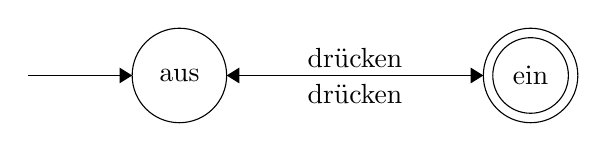
\begin{tikzpicture}[scale=0.2]
\tikzstyle{every node}+=[inner sep=0pt]
\draw [black] (23.8,-28.8) circle (3);
\draw (23.8,-28.8) node {aus};
\draw [black] (46.1,-28.8) circle (3);
\draw (46.1,-28.8) node {ein};
\draw [black] (46.1,-28.8) circle (2.4);
\draw [black] (26.8,-28.8) -- (43.1,-28.8);
\fill [black] (43.1,-28.8) -- (42.3,-28.3) -- (42.3,-29.3);
\draw (34.95,-29.3) node [below] {drücken};
\draw [black] (43.1,-28.8) -- (26.8,-28.8);
\fill [black] (26.8,-28.8) -- (27.6,-29.3) -- (27.6,-28.3);
\draw (34.95,-28.3) node [above] {drücken};
\draw [black] (14.2,-28.8) -- (20.8,-28.8);
\fill [black] (20.8,-28.8) -- (20,-28.3) -- (20,-29.3);
\end{tikzpicture}
\end{center}

\begin{definition}[Endlicher Automat]
Wir haben: \begin{itemize}
\item Zwei Zustände, davon ein Startzustand
\item und ein akzeptierender Zustand
\item Transitionen (Zustandsübergänge): führen den Automaten anhand einer Eingabe von einem Zusand in den nächsten.
\end{itemize}
\end{definition}

Beispiel: Mustererkennung in Texten: z.B. Suche das Wort "then"

\begin{center}
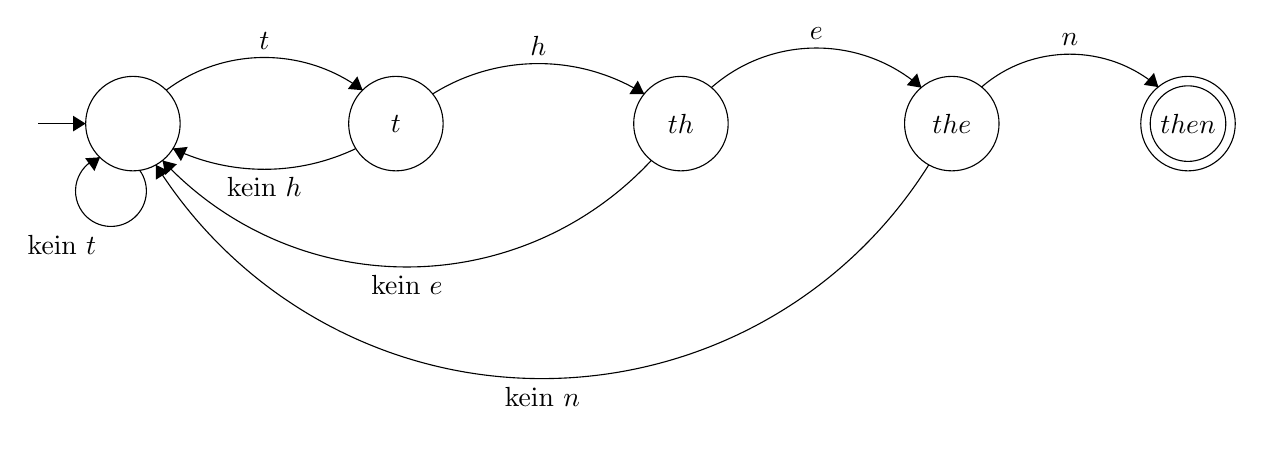
\begin{tikzpicture}[scale=0.2]
\tikzstyle{every node}+=[inner sep=0pt]
\draw [black] (7.4,-27.9) circle (3);
\draw [black] (24.1,-27.9) circle (3);
\draw (24.1,-27.9) node {$t$};
\draw [black] (42.2,-27.9) circle (3);
\draw (42.2,-27.9) node {$th$};
\draw [black] (59.4,-27.9) circle (3);
\draw (59.4,-27.9) node {$the$};
\draw [black] (74.4,-27.9) circle (3);
\draw (74.4,-27.9) node {$then$};
\draw [black] (74.4,-27.9) circle (2.4);
\draw [black] (1.4,-27.9) -- (4.4,-27.9);
\fill [black] (4.4,-27.9) -- (3.6,-27.4) -- (3.6,-28.4);
\draw [black] (9.509,-25.781) arc (126.87812:53.12188:10.4);
\fill [black] (21.99,-25.78) -- (21.65,-24.9) -- (21.05,-25.7);
\draw (15.75,-23.2) node [above] {$t$};
\draw [black] (26.43,-26.021) arc (122.09355:57.90645:12.649);
\fill [black] (39.87,-26.02) -- (39.46,-25.17) -- (38.93,-26.02);
\draw (33.15,-23.59) node [above] {$h$};
\draw [black] (44.128,-25.616) arc (131.3237:48.6763:10.104);
\fill [black] (57.47,-25.62) -- (57.2,-24.71) -- (56.54,-25.46);
\draw (50.8,-22.6) node [above] {$e$};
\draw [black] (61.283,-25.584) arc (130.87735:49.12265:8.583);
\fill [black] (72.52,-25.58) -- (72.24,-24.68) -- (71.59,-25.44);
\draw (66.9,-22.99) node [above] {$n$};
\draw [black] (7.827,-30.858) arc (35.95699:-252.04301:2.25);
\draw (2.89,-34.93) node [below] {kein $t$};
\fill [black] (5.31,-30.04) -- (4.37,-30.1) -- (4.96,-30.91);
\draw [black] (21.56,-29.484) arc (-64.4345:-115.5655:13.463);
\fill [black] (9.94,-29.48) -- (10.45,-30.28) -- (10.88,-29.38);
\draw (15.75,-31.3) node [below] {kein $h$};
\draw [black] (40.321,-30.235) arc (-42.87511:-137.12489:21.179);
\fill [black] (9.28,-30.24) -- (9.46,-31.16) -- (10.19,-30.48);
\draw (24.8,-37.5) node [below] {kein $e$};
\draw [black] (57.939,-30.519) arc (-32.11581:-147.88419:28.973);
\fill [black] (8.86,-30.52) -- (8.86,-31.46) -- (9.71,-30.93);
\draw (33.4,-44.59) node [below] {kein $n$};
\end{tikzpicture}
\end{center}

Getränkeautomat (Beispiel für Automat mit Ausgabe): Cola für CHF 2, Wasser für CHF 1. Münzannahme: Münzen zu 1, 2 CHF.

\begin{center}
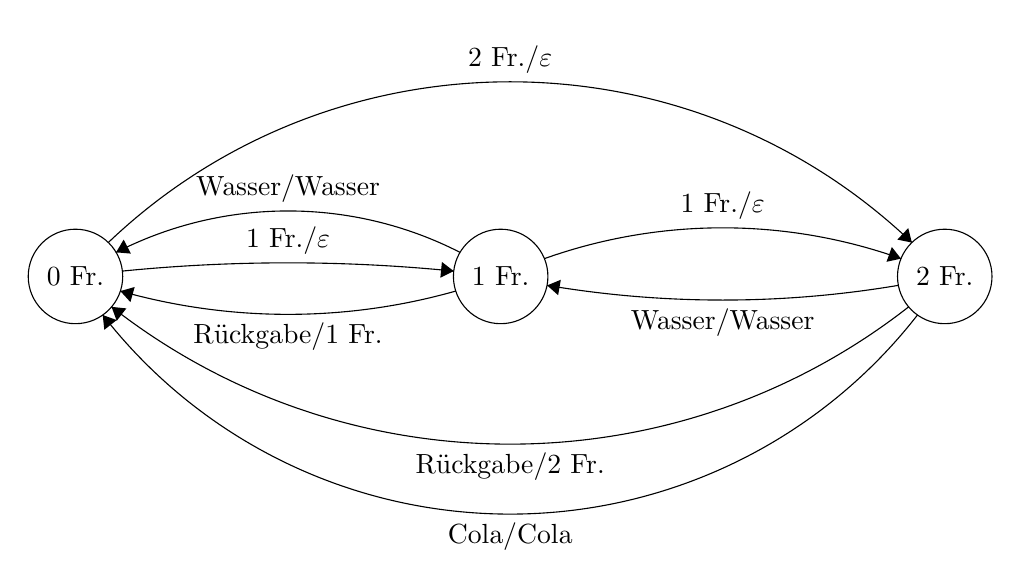
\begin{tikzpicture}[scale=0.2]
\tikzstyle{every node}+=[inner sep=0pt]
\draw [black] (8.2,-27.2) circle (3);
\draw (8.2,-27.2) node {$0$ Fr.};
\draw [black] (35.2,-27.2) circle (3);
\draw (35.2,-27.2) node {$1$ Fr.};
\draw [black] (63.4,-27.2) circle (3);
\draw (63.4,-27.2) node {$2$ Fr.};
\draw [black] (11.181,-26.859) arc (95.70544:84.29456:105.815);
\fill [black] (32.22,-26.86) -- (31.47,-26.28) -- (31.37,-27.28);
\draw (21.7,-25.84) node [above] {$1$ Fr./$\varepsilon$};
\draw [black] (37.977,-26.069) arc (109.61489:70.38511:33.729);
\fill [black] (60.62,-26.07) -- (60.04,-25.33) -- (59.7,-26.27);
\draw (49.3,-23.61) node [above] {$1$ Fr./$\varepsilon$};
\draw [black] (10.286,-25.045) arc (133.60946:46.39054:36.991);
\fill [black] (61.31,-25.05) -- (61.08,-24.13) -- (60.39,-24.86);
\draw (35.8,-14.34) node [above] {$2$ Fr./$\varepsilon$};
\draw [black] (32.348,-28.128) arc (-74.17617:-105.82383:39.049);
\fill [black] (11.05,-28.13) -- (11.69,-28.83) -- (11.96,-27.87);
\draw (21.7,-30.11) node [below] {Rückgabe/$1$ Fr.};
\draw [black] (61.106,-29.132) arc (-51.98339:-128.01661:41.089);
\fill [black] (10.49,-29.13) -- (10.82,-30.02) -- (11.43,-29.23);
\draw (35.8,-38.35) node [below] {Rückgabe/$2$ Fr.};
\draw [black] (10.779,-25.671) arc (117.08879:62.91121:23.983);
\fill [black] (10.78,-25.67) -- (11.72,-25.75) -- (11.26,-24.86);
\draw (21.7,-22.54) node [above] {Wasser/Wasser};
\draw [black] (61.668,-29.648) arc (-37.90364:-142.09636:32.784);
\fill [black] (9.93,-29.65) -- (10.03,-30.59) -- (10.82,-29.97);
\draw (35.8,-42.79) node [below] {Cola/Cola};
\draw [black] (60.454,-27.765) arc (-80.41933:-99.58067:67.017);
\fill [black] (38.15,-27.77) -- (38.85,-28.39) -- (39.02,-27.41);
\draw (49.3,-29.2) node [below] {Wasser/Wasser};
\end{tikzpicture}
\end{center}

Wenn der Automat nur eine Flasche Cola und eine Flasche Wasser enthält:

\begin{center}
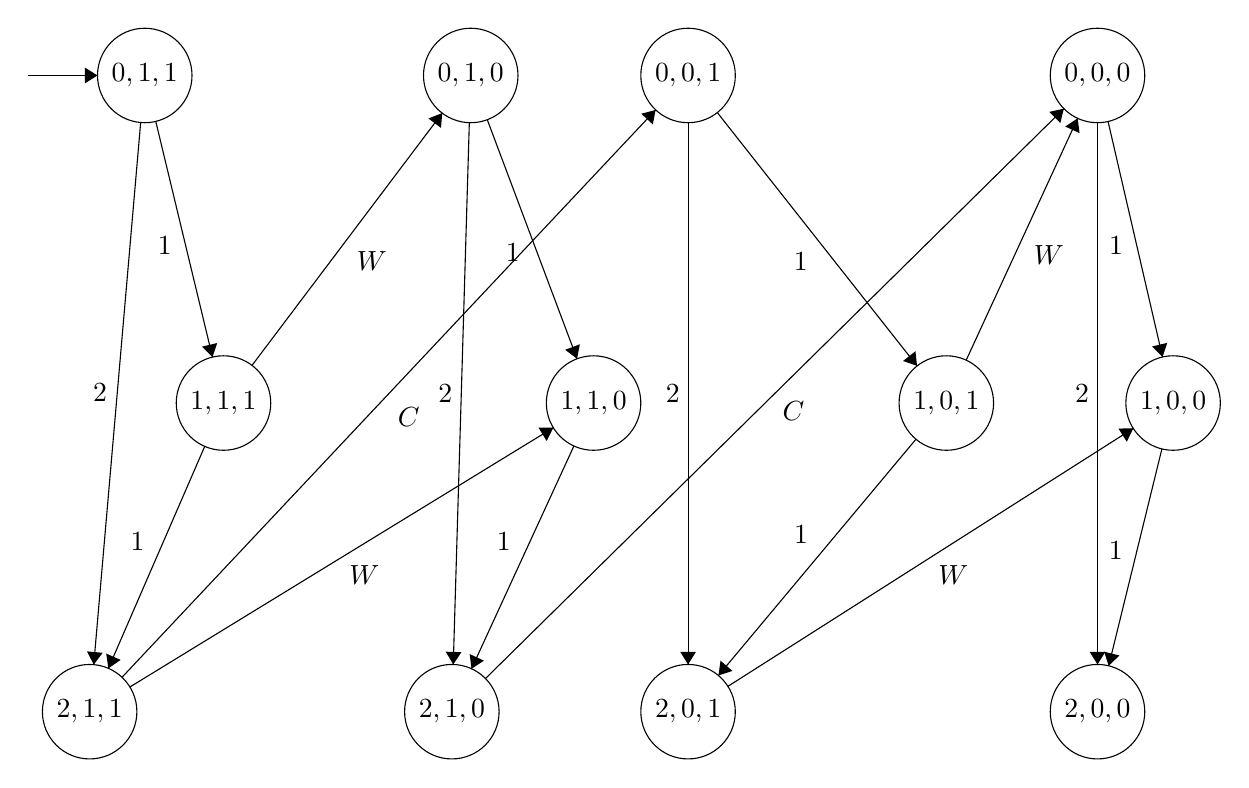
\begin{tikzpicture}[scale=0.2]
\tikzstyle{every node}+=[inner sep=0pt]
\draw [black] (9.8,-7.7) circle (3);
\draw (9.8,-7.7) node {$0,1,1$};
\draw [black] (30.5,-7.7) circle (3);
\draw (30.5,-7.7) node {$0,1,0$};
\draw [black] (44.3,-7.7) circle (3);
\draw (44.3,-7.7) node {$0,0,1$};
\draw [black] (14.8,-28.5) circle (3);
\draw (14.8,-28.5) node {$1,1,1$};
\draw [black] (38.3,-28.5) circle (3);
\draw (38.3,-28.5) node {$1,1,0$};
\draw [black] (60.7,-28.5) circle (3);
\draw (60.7,-28.5) node {$1,0,1$};
\draw [black] (70.3,-7.7) circle (3);
\draw (70.3,-7.7) node {$0,0,0$};
\draw [black] (75.1,-28.5) circle (3);
\draw (75.1,-28.5) node {$1,0,0$};
\draw [black] (6.3,-48.1) circle (3);
\draw (6.3,-48.1) node {$2,1,1$};
\draw [black] (29.3,-48.1) circle (3);
\draw (29.3,-48.1) node {$2,1,0$};
\draw [black] (44.3,-48.1) circle (3);
\draw (44.3,-48.1) node {$2,0,1$};
\draw [black] (70.3,-48.1) circle (3);
\draw (70.3,-48.1) node {$2,0,0$};
\draw [black] (2.4,-7.7) -- (6.8,-7.7);
\fill [black] (6.8,-7.7) -- (6,-7.2) -- (6,-8.2);
\draw [black] (10.5,-10.62) -- (14.1,-25.58);
\fill [black] (14.1,-25.58) -- (14.4,-24.69) -- (13.43,-24.92);
\draw (11.54,-18.53) node [left] {$1$};
\draw [black] (9.54,-10.69) -- (6.56,-45.11);
\fill [black] (6.56,-45.11) -- (7.13,-44.36) -- (6.13,-44.27);
\draw (7.43,-27.83) node [left] {$2$};
\draw [black] (31.55,-10.51) -- (37.25,-25.69);
\fill [black] (37.25,-25.69) -- (37.43,-24.77) -- (36.5,-25.12);
\draw (33.64,-18.92) node [left] {$1$};
\draw [black] (30.41,-10.7) -- (29.39,-45.1);
\fill [black] (29.39,-45.1) -- (29.91,-44.32) -- (28.91,-44.29);
\draw (29.36,-27.89) node [left] {$2$};
\draw [black] (44.3,-10.7) -- (44.3,-45.1);
\fill [black] (44.3,-45.1) -- (44.8,-44.3) -- (43.8,-44.3);
\draw (43.8,-27.9) node [left] {$2$};
\draw [black] (46.16,-10.06) -- (58.84,-26.14);
\fill [black] (58.84,-26.14) -- (58.74,-25.21) -- (57.95,-25.83);
\draw (51.93,-19.52) node [left] {$1$};
\draw [black] (70.3,-10.7) -- (70.3,-45.1);
\fill [black] (70.3,-45.1) -- (70.8,-44.3) -- (69.8,-44.3);
\draw (69.8,-27.9) node [left] {$2$};
\draw [black] (70.97,-10.62) -- (74.43,-25.58);
\fill [black] (74.43,-25.58) -- (74.73,-24.68) -- (73.76,-24.91);
\draw (71.95,-18.5) node [left] {$1$};
\draw [black] (13.61,-31.25) -- (7.49,-45.35);
\fill [black] (7.49,-45.35) -- (8.27,-44.81) -- (7.35,-44.41);
\draw (9.82,-37.33) node [left] {$1$};
\draw [black] (37.05,-31.23) -- (30.55,-45.37);
\fill [black] (30.55,-45.37) -- (31.34,-44.86) -- (30.43,-44.44);
\draw (33.08,-37.28) node [left] {$1$};
\draw [black] (58.77,-30.8) -- (46.23,-45.8);
\fill [black] (46.23,-45.8) -- (47.12,-45.51) -- (46.36,-44.86);
\draw (51.95,-36.86) node [left] {$1$};
\draw [black] (74.39,-31.41) -- (71.01,-45.19);
\fill [black] (71.01,-45.19) -- (71.69,-44.53) -- (70.72,-44.29);
\draw (71.94,-37.86) node [left] {$1$};
\draw [black] (16.61,-26.11) -- (28.69,-10.09);
\fill [black] (28.69,-10.09) -- (27.81,-10.43) -- (28.61,-11.03);
\draw (23.23,-19.5) node [right] {$W$};
\draw [black] (8.86,-46.53) -- (35.74,-30.07);
\fill [black] (35.74,-30.07) -- (34.8,-30.06) -- (35.32,-30.91);
\draw (23.74,-38.8) node [below] {$W$};
\draw [black] (8.36,-45.91) -- (42.24,-9.89);
\fill [black] (42.24,-9.89) -- (41.33,-10.13) -- (42.06,-10.81);
\draw (25.83,-29.37) node [right] {$C$};
\draw [black] (31.44,-45.99) -- (68.16,-9.81);
\fill [black] (68.16,-9.81) -- (67.24,-10.01) -- (67.94,-10.72);
\draw (50.99,-28.38) node [below] {$C$};
\draw [black] (61.96,-25.78) -- (69.04,-10.42);
\fill [black] (69.04,-10.42) -- (68.25,-10.94) -- (69.16,-11.36);
\draw (66.22,-19.13) node [right] {$W$};
\draw [black] (46.83,-46.49) -- (72.57,-30.11);
\fill [black] (72.57,-30.11) -- (71.63,-30.12) -- (72.16,-30.96);
\draw (61.14,-38.8) node [below] {$W$};
\end{tikzpicture}
\end{center}

\section{Formale Sprachen}

Ziel: Genaue Beschreibung der Ein- und Ausgaben eines Automaten.

\begin{definition}[Alphabet]
(endliche, nichtleere Menge von Symbolen). Bsp: Binäres Alphabet $\Sigma_{\textrm{bin}} = \{0,1\}$, Tastaturalphabet $\Sigma_{\textrm{tast}} = \{ a, \dots, z, A, \dots, Z, 0, \dots 9, \dots \}$
\end{definition}

\begin{definition}[Wort (= Zeichenkette, String)]
Endliche Folge von Symbolen eines gegebenen Alphabets. Beispiel: 01110 ist ein Wort über $\Sigma_{\textrm{bin}}$.
\end{definition}

\begin{bemerkung}[Eigenschaften von Wörtern]
Die da wären:
\begin{itemize}
\item Leeres Wort: $\varepsilon$ (manchmal $\lambda$) = leere Folge von Symbolen (über einem beliebigen Alphabet)
\item Länge eines Wortes: $|w|$ bezeichnet die Anzahl der Symbole im Wort $w$. $|\varepsilon| = 0$.
\end{itemize}
\end{bemerkung}

\begin{bemerkung}[Konventionen für Darstellung von Wörtern]
Wir sagen:
\begin{itemize}
\item $a,b,c,\dots$ für Buchstaben, Symbole
\item $v,w,x,\dots$ für Wörter
\end{itemize}
\end{bemerkung}

\begin{definition}[Potenzen von Wörtern]
Es gibt im Angebot:
\begin{itemize}
\item Menge aller Wörter einer bestimmten Länge:
\begin{eqnarray*}
\textrm{Sei $\Sigma$ Alphabet, so:} && \\
 \Sigma^0 &=& \{\varepsilon\} \\
 \Sigma^1 &=& \Sigma \\
\Sigma^2 &=& \{ ab | a,b \in \Sigma\} \\
\Sigma^i &=& \{ a_1\dots a_i | a_1 \dots a_i \in \Sigma \}
\end{eqnarray*}
\item Menge aller Wörter über $\Sigma$: \[
\Sigma^* = \bigcup\limits_{i = 0}^{\infty} \Sigma^i, \varepsilon \in \Sigma^*
\]
\item Menge aller nichtleeren Wörter über $\Sigma$: \[
\Sigma^+ = \bigcup\limits_{i = 1}^{\infty} \Sigma^i, \varepsilon \notin \Sigma^+
\]
\end{itemize}
\end{definition}
\begin{beispiel}
\item Beispiel: \begin{eqnarray*}
\Sigma &=& \{0,1\} \\
\Sigma^2 &=& \{00, 01, 10, 11\} \\
\Sigma^* &=& \{\varepsilon, 0, 1, 00, 01, 10, 11, 000, 001, \dots \}
\end{eqnarray*}
\end{beispiel}

\begin{definition}[Konkatenation (Verkettung) von Wörtern]
\[
v = a_1,\dots a_k, w = b_1\dots,b_k \textrm{ über } \Sigma \Rightarrow v\cdot w = a_1\dots a_kb_1\dots b_k = vw
\]
\end{definition}

\begin{bemerkung}[Rechenregeln für Konkatenation von Wörtern]
\begin{eqnarray*}
v\cdot(v\cdot w) &=& (u\cdot v)\cdot w \\
|x\cdot y| &=& |x| + |y| \\
x\cdot\varepsilon&=&\varepsilon\cdot x =  x
\end{eqnarray*}
\end{bemerkung}

\begin{bemerkung}[Infixe, Präfixe, Suffixe]
Seien $v,w \in \Sigma^*$ für ein Alphabet $\Sigma$, dann ist $v$ ein Teilwort (Infix) von $w$, falls es $x,y \in \Sigma^*$ gibt, so dass $w = x\cdot v \cdot y$; $v$ ist ein Präfix von $w$, falls es $y \in \Sigma^*$ gibt, so dass $w = v\cdot y$. Suffix funktionert analog.

Beispiel: abc ist Teilwort von aabcc, aa ist Präfix und Suffix von aabcaa. $\varepsilon$ ist Teilwort von jedem Wort.
\end{bemerkung}

\begin{definition}[Sprache]
$L$ über Alphabet $\Sigma$ ist eine Teilmenge von $\Sigma^*$, $L \subseteq \Sigma^*$. Sprache ist Menge von Wörtern, kann unendlich gross sein. Leere Sprache: $\varnothing$ enthält keine Wörter, ist über jedem Alphabet definiert. Spezielle Sprache: $L_\varepsilon$ ist die Sprache, die nur das leeere Wort enthält. $L_\varepsilon \neq \varnothing$.
\end{definition}

\begin{definition}[Konkatenation von Sprachen] 
$L_1, L_2 \subseteq \Sigma^* \Rightarrow L_1 \cdot L_2 = L_1L_2 = \{ v\cdot w | v\in L_1, w\in L_2 \}$
\end{definition}
\begin{definition}[Potenzen von Sprachen]
\begin{eqnarray*}
L^0 &=& L_\varepsilon = \{\varepsilon\} \\
L^{i+1} &=& L^i\cdot L \textrm{ für } i \in \mathbb{N}
\end{eqnarray*}
\end{definition}

\begin{definition}[Kleene-Stern] 
\begin{eqnarray*}
L^* &=& \bigcup\limits_{i\in \mathbb{N}}^{} L^i \\
L^+ &=& \bigcup\limits_{i\in \mathbb{N}}^{} L^i - L_\varepsilon
\end{eqnarray*}
\end{definition}

\begin{beispiel}
Sei $\Sigma = \{a,b\}, L_1 = \{a^i | i \ge 0\} = \{\varepsilon, a, aa, aaa, \dots\}, L_2 = \{b^i | i \ge 0\} = \{\varepsilon, b, bb, bbb, \dots\}$:

$L_1\cdot L_2 = \{ \varepsilon, a,b,ab,aab,abb,aaab,\dots \} = \{a^ib^j | i \ge 0, j \ge 0 \}$ ist die Menge aller Wörter über $\{a,b\}$, in dem alle $a$s vor allen $b$s vorkommen.
\end{beispiel}

\begin{ubung}
Seien $L_1, L_2, L_3 \subseteq \Sigma^*$. 

(a) Gilt $(L_1\cdot L_2)\cdot L_3 =L_1\cdot(L_2\cdot L_3 )$? Ja.

(b) Gilt $(L_1\cup L_2)\cdot L_3 = L_1\cdot L_3 \cup L_2 \cdot L_3$? Ja.

(c) Gilt $(L_1\cdot L_2)\cup L_3 = (L_1\cup L_3) \cdot (L_2\cup L_3)$? Quatsch.

(d) Gilt $L_1\cdot L_2 = L_2\cdot L_1$? Quatsch.

\end{ubung}

\begin{proof}[Beweis]
(a)
\begin{eqnarray*}
(L_1\cdot L_2) \cdot L_3 &=& \{ vw | v \in L_1\cdot L_2, w \in L_3 \} \\
&=&\{xyw | x\in L_1, y \in L_2, w \in L_3 \} \\
&=& \{xz | x \in L_1, z \in L_2 L_3 \} \\
&=& L_1\cdot (L_2\cdot L_3)
\end{eqnarray*}

(b)
\begin{eqnarray*}
(L_1 \cup L_2) \cdot L_3 &=& \{vw | v \in L_1 \cup L_2, w \in L_3 \} \\
&=& \{vw | v \in L_1, w \in L_3 \} \cup \{ vw | v \in L_2, w \in L_3 \} \\
&=& (L_1\cdot L_3) \cup (L_2 \cdot L_3)
\end{eqnarray*}

(c)
Gegenbeispiel: $L_1 = L_2 = \{a\}, L_3 = \{b \}$. Daraus folgt:
\begin{eqnarray*}
L_1 L_2 = \{aa\} &\Rightarrow& (L_1 L_2)\cup L_3 = \{aa,b \} \\
L_1 \cup L_3 = \{a,b\} = L_2 \cup L_3 &=& \Rightarrow ...
\end{eqnarray*}

\end{proof}

\begin{bemerkung}
(d) gilt aber für $|\Sigma|$ = 1.
\end{bemerkung}

\begin{definition}[Entscheidungsproblem]
Die Eingabe ist eine Sprache $L$ über einem Alphabet $\Sigma$ sowie ein Wort $w \in \Sigma^*$. Die Ausgabe soll lauten: JA falls $w \in L$ oder NEIN falls $w \notin L$.

Die Modellierung von vielen alltäglichen Berechnungsproblemen im Formalismus der formalen Sprachen.
\end{definition}

\begin{beispiel}[Primzahltest]
Das Alphabet $\Sigma = \{0,1\}$. Die Sprache 
\[
L = \{w \in \Sigma^* | w \textrm{ ist Binärdarstellung einer Primzahl}  \}
\]

Eine Zahl $p \in N$ ist Primzahl genau dann, wenn $Bin(p) \in L$.

Identifizierung von Sprachen als Probleme.
\end{beispiel}

\section{Kurze Einführung in formale Beweise}

Behauptungen\footnote{11. September 2012} mit Unanfechtbarkeitsanspruch wollen bewiesen werden. Insbesondere negative Aussagen der Form "Dieses Rechenmodell kann diese Aufgabe nicht lösen" brauchen eine präzise Formulierung und Begründung, um glaubwürdig zu sein\footnote{Hopcraft et al., Abschnitt 1.2--1.4}\marginpar{Unkontrollierte Hausaufgabe}.

Als Beweismethoden haben wir im Angebot:

\begin{description}
\item[Deduktion (zum Beweis einer Implikation)] Zum Beweis von Wenn-Dann-Aussagen, z.B.
\[
\textrm{Wenn } \underbrace{x \ge 4}_{\textrm{Hypothese}}\textrm{ , dann } \underbrace{x^2\ge 16}_{\textrm{Konklusion}}
\]

Vorgehen: Hypothese als wahr annehmen, dann Folgerungen darauf anwenden, bis die Konklusion folgt.

\begin{beispiel}
Sei $x \ge 4$. Es gilt $4^2 = 16$ und die Quadratfunktion ist steigend. Daraus folgt: $x^2 \ge 4^2 = 16$
\end{beispiel}

Hierfür ist es oft hilfreich, Definitionen von Begriffen einzusetzen.
\begin{beispiel}
Wenn $L = \{ w \in \{a,b\}^* | |w| \textrm{ gerade}\}$, dann gilt für alle $x \in L^2$, dass $|x|$ gerade ist.
\end{beispiel}

\begin{proof}[Beweis]
Sei $x \in L^2$.

Definition von $L^2$ einsetzen. Es existieren $u,v \in L$, so dass $x = uv$.

Definition von $L$ einsetzen. $|u|$ ist gerade, $|v|$ ist gerade.

$\Rightarrow |x| = |u| + |v| \Rightarrow |x|$ ist gerade.
\end{proof}

\item[Doppelte Deduktion (zum Beweis einer Äquivalenz)] Zerlegung in zwei Wenn-Dann-Aussagen, wird getrennt bewiesen.

\begin{beispiel}[Gleichheit von Mengen]
\[
A = B \Rightarrow A \subseteq B \land B \subseteq A \Rightarrow A = B
\]

\end{beispiel}

\begin{beispiel}
Sprachen sind ja auch Mengen. Also: seien $L_1, L_2 \in \Sigma^*$. Dann gilt:
\[
L_1\cdot(L_1 \cup L_2) = L_1^2 \cup L_1 \cdot L_2
\]
\end{beispiel}

\begin{proof}[Beweis]
\begin{itemize}
Zweimal:
\item "$\subseteq$":

Sei $x \in L_1\cdot(L_1\cup L_2) \Rightarrow \exists x = uv, u \in L_1, v \in L_1 \cup L_2$.

Fallunterscheidung: (a) $v \in L_1 \Rightarrow x = uv, u \in L_1, v \in L_1 \Rightarrow x \in L_1^2$.

(b) $v \in L_2 \Rightarrow x = uv, u \in L_1, v \in L_2 \Rightarrow x \in L_1\cdot L_2$.

\item "$\supseteq$":

Sei $x \in L_1^2 \cup L_1\cdot L_2$.

Fallunterscheidung: (a) $x \in L_1^2 \Rightarrow x = uv, u, v \in L_1 $

$\Rightarrow v \in L_1 \cup L_2$

$\Rightarrow x \in L_1\cdot(L_1 \cup L_2)$.

(b) $x \in L_1\cdot L_2 \Rightarrow x = uv, u \in L_1, v \in L_2$

$\Rightarrow v \in (L_1 \cup L_2)$

$\Rightarrow x \in L_1\cdot(L_1 \cup L_2)$
\end{itemize}
\end{proof}

\item[Widerspruchsbeweis] Es wird eine Annahme getroffen und dann solange gefolgert, bis Quatsch herauskommt. Daraus folgt, dass die Annahme auch falsch sein muss.

\begin{beispiel}
Seien $a,b \in \mathbb{N}$ und $a,b \ge 2$. Dann gilt: $a$ teilt nicht $ab + 1$.
\end{beispiel}
\begin{proof}[Beweis]
Seien $a,b \in \mathbb{N}$. Angenommen, $a$ teilt $ab + 1$.

Ziel: Annahme zum Widerspruch führen, dann folgt daraus Negation, also die gewünschte Konklusion.

$a$ teilt $ab \Rightarrow a$ teilt $ab$ und $ab + 1$.

$\Rightarrow a$ teilt $(ab + 1)-(ab) = 1$

$\Rightarrow a = 1$. Bonk! Widerspruch zu $a \ge 2$.
\end{proof}

\begin{beispiel}
Es gibt unendlich viele Primzahl (äquivalente Formulierung: Es gibt keine grösste Primzahl).
\end{beispiel}

\begin{proof}[Beweis]
Angenommen, es gäbe eine grösste Primzahl. Wir nennen die Anzahl der Primzahlen $k$.

Seien $p_1 < p_2 < \dots < p_k$ die Primzahlen. Betrachten wir $x = p_1\cdot p_2 \cdot \dots \cdot p_k + 1$. Da $p_k$ die grösste Primzahl ist und $x > p_k$, kann $x$ keine Primzahl sein.

Also gibt es eine Primfaktorzerlegung von $x$, und $p_l$ sei die kleinste Primzahl in dieser Zerlegung.

Dann gilt: $p_l$ teilt $p_1\cdot p_2 \cdot dots \cdot p_k$ und $p_l$ teilt darum auch $x$.

Daraus folgt: $p_l$ teilt  $p_1\cdot p_2 \cdot dots \cdot p_k+1$. Aus dem vorhergehenden Beweis ($a$ teilt $ab+1$) folgt, dass das ein Widerspruch ist.
\end{proof}

\item[Induktion] Vor allem verwendet für Beweise über natürliche Zahlen. Ziel: Zeige, dass die Aussage $S(n)$ für alle $n \ge n_0$ gilt.

Methode:
\begin{enumerate}
\item Induktionsanfang (Anker). Zeige $S(n_0)$.
\item Induktionsschritt. Zeige $S(i) \Rightarrow S(i+1)$.
\end{enumerate}

Idee: Wenn $S(n_0)$ gilt und $S(i) \Rightarrow S(i+1)$ für alle $i \ge n_0$, dann folgt aus $S(n_0)$ und $S(n_0) \Rightarrow S(n_0+1)$, dann gilt $S(n_0+1)$. Undsoweiter, undsofort.

\begin{beispiel}[Der kleine Gauss].
Für alle $n \ge 1$ gilt: $\sum\limits_{i=1}^n i = \frac {n(n+1)} 2$
\end{beispiel}
\begin{proof}[Beweis]
Anker: $\sum\limits_{i=1}^1 = \frac{1+(1+1)}2$

Schritt: es gelte $\sum\limits_{i=1}^k i = \frac{k(k+1)} 2$ (Induktionsvoraussetzung).

Zeige: $\sum\limits_{i=1}^{k+1} i = \frac{(k+1)(k+1+1)} 2$ (Induktionsbehauptung).

\begin{eqnarray*}
\sum\limits_{i=1}^{k+1} i &=& \sum\limits_{i=1}^{k} i + (k+1) \\
&=& \frac{k(k+1)} 2 + (k+1) \\
&=& \frac{k(k+1) + 2(k+1)}2 \\
&=& \frac{(k+2)(k+1)}2 \\
&=& \frac{(k+1+1)(k+1)}2
\end{eqnarray*}
\end{proof}

\item[Rekursive Definitionen und strukturelle Induktion]
\begin{beispiel}[Rekursive Definition von arithmetischen Ausdrücken]
Basis: Jede Zahl und jede Variable ist ein arithmetischer Ausdruck: $(a+3)\cdot 5$ ist ein arithmetischer Ausdruck, $(a +3\cdot 5$ [sic] ist keiner (Klammerfehler).

Rekursion: Wenn $E$ und $F$ Ausdrücke sind, dann definieren wir, dass dann auch $E+F$, $E\cdot F$, $(E)$ arithmetische Ausdrücke sind.

Behauptung: Jeder Ausdruck enthält gleichviele linke wie rechte Klammern.
\end{beispiel}

\begin{proof}[Beweis] Mit struktureller Induktion:

\begin{enumerate}
\item I.A.: Basisausdrücke haben keine Klammern. Daraus folgt: gleichviele linke wie rechte Klammern (0).
\item Sei $G$ ein arithmetischer Ausdruck ($G = E+F, E\cdot F, (G)$). Fallunterscheidung:
\begin{enumerate}
\item $G=E+F$: Induktionsvoraussetzung: $E$ und $F$ haben gleich viele linke wie rechte Klammern. Gilt also auch für $G$, da keine Klammern hinzukommen.
\item $G=E\cdot F$: analog.
\item $(G)$: Induktionsvoraussetzung: $E$ hat gleich viele linke wie rechte Klammern. Gilt also auch für $G$, da 1 linke und 1 rechte Klammer hinzukommt.
\end{enumerate}
\end{enumerate}
\end{proof}

\end{description}

\section{Unendlichkeit}

\begin{proof}[Beweis für 3.7]
Behauptung: $|A| < |B| \Leftarrow |A| = |C| \land C \subset B$

$A = B = \mathbb{N} = \{0,1,2,3,\dots\}$
$C = \{1,2,3,4,\dots\}$
$(0,1), (1,2), \dots, (k,k+1)$
\end{proof}

Aufgaben: 3.7, 3.8, 3.11, 3.17, 3.18, 3.19

\section{Endliche Automaten}

Unterscheidung:
\begin{description}
\item[Deterministisch] Automat kann zu einem Zeitpunkt nur einen Zustand annehmen.
\item[Nichtdeterministisch] Automat kann gleichzeitig mehrere Zustände besitzen.
\end{description}

\begin{beispiel}
DEA zum Erkennen des Musters aba:

\begin{center}
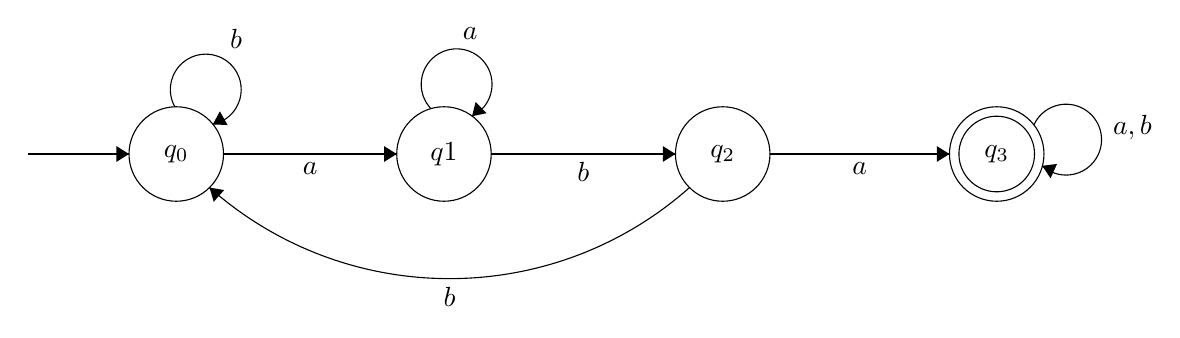
\begin{tikzpicture}[scale=0.2]
\tikzstyle{every node}+=[inner sep=0pt]
\draw [black] (15.3,-25.4) circle (3);
\draw (15.3,-25.4) node {$q_0$};
\draw [black] (32.3,-25.4) circle (3);
\draw (32.3,-25.4) node {$q1$};
\draw [black] (50,-25.4) circle (3);
\draw (50,-25.4) node {$q_2$};
\draw [black] (67.4,-25.4) circle (3);
\draw (67.4,-25.4) node {$q_3$};
\draw [black] (67.4,-25.4) circle (2.4);
\draw [black] (5.9,-25.4) -- (12.3,-25.4);
\fill [black] (12.3,-25.4) -- (11.5,-24.9) -- (11.5,-25.9);
\draw [black] (18.3,-25.4) -- (29.3,-25.4);
\fill [black] (29.3,-25.4) -- (28.5,-24.9) -- (28.5,-25.9);
\draw (23.8,-25.9) node [below] {$a$};
\draw [black] (35.3,-25.4) -- (47,-25.4);
\fill [black] (47,-25.4) -- (46.2,-24.9) -- (46.2,-25.9);
\draw (41.15,-25.9) node [below] {$b$};
\draw [black] (53,-25.4) -- (64.4,-25.4);
\fill [black] (64.4,-25.4) -- (63.6,-24.9) -- (63.6,-25.9);
\draw (58.7,-25.9) node [below] {$a$};
\draw [black] (15.214,-22.413) arc (209.37644:-78.62356:2.25);
\draw (19.09,-18.76) node [above] {$b$};
\fill [black] (17.62,-23.52) -- (18.56,-23.56) -- (18.07,-22.69);
\draw [black] (31.478,-22.527) arc (223.69515:-64.30485:2.25);
\draw (33.97,-18.17) node [above] {$a$};
\fill [black] (34.08,-23) -- (35,-22.81) -- (34.31,-22.09);
\draw [black] (47.892,-27.531) arc (-48.4339:-131.5661:22.972);
\fill [black] (17.41,-27.53) -- (17.68,-28.44) -- (18.34,-27.69);
\draw (32.65,-33.82) node [below] {$b$};
\draw [black] (69.756,-23.562) arc (155.68937:-132.31063:2.25);
\draw (74.75,-23.7) node [right] {$a,b$};
\fill [black] (70.29,-26.15) -- (70.82,-26.94) -- (71.23,-26.03);
\end{tikzpicture}
\end{center}

Zustände speichern das bereits gelesene Teilmuster:

\begin{itemize}
\item $q_0$: noch nichts vom Teilwort aba gelesen.
\item $q_1$: zumindest schon das Wort a gelesen.
\item $q_2$: schon ab gelesen.
\item $q_3$: das ganze Muster gelesen, es kann also akzeptiert werden.
\end{itemize}
\end{beispiel}

Transitionen (Zustandsübergänge£) beschreiben die Änderung beim Lesen eines Zeichens des Wortes.

\begin{definition}[Formale Definition (nochmal)]
Ein DEA $A$ wird beschrieben durch $A = (Q, \Sigma, \delta, q_0, F)$, wobei:
\begin{itemize}
\item $Q$ ist eine endliche Menge von Zuständen,
\item $\Sigma$ ist das Alphabet für die Eingabe,
\item $q_0$ ist der Startzustand, $q_0 \in Q$,
\item $F$ ist die Menge der akzeptierenden Zustände (Endzustände), $F \subseteq Q$,
\item $\delta: Q \times \Sigma \mapsto Q$ ist die Übergangsfunktion (Transitionsfunktion), die für jeden Zustand und jedes Eingabesymbol einen eindeutigen Folgezustand definiert.

\end{itemize}
\end{definition}

\begin{beispiel}[von vorher]
\[
A = \left( \{q_0, q_1, q_2, q_3\}, \{ a,b\}, \delta, q_0, \{q_3 \} \right),
\]

wobei $\delta$ gegeben ist durch:

\begin{eqnarray*}
\delta(q_0, a) = q_1, \\
\delta(q_0, b) = q_0, \\
\delta(q_1, a) = q_1, \\
\delta(q_1, b) = q_2, \\
\delta(q_2, a) = q_3, \\
\delta(q_2, b) = q_0, \\
\delta(q_3, a) = q_3, \\
\delta(q_3, b) = q_3 \\
\end{eqnarray*}

(oder als Transitionstabelle aufgeschrieben):

\begin{tabular}{r|cc}
 & $a$ & $b$ \\
\hline 
$\mapsto q_0$ & $q_1$ & $q_0$ \\
$q_1$ & $q_1$ & $q_2$ \\
$q_2$ & $q_3$ & $q_0$ \\
$*q_3$ & $q_3$ & $q_3$
\end{tabular}

\end{beispiel}

Die Transitionstabelle enthält alle Informationen über einen DEA, meistens ist aber die graphische Darstellung übersichtlicher.

Ziel: Automaten zur Beschreibung von Sprachen verwenden.

\begin{definition}[Berechnung]
Sei $A = (Q, \Sigma, \delta, q_0, F)$ ein DEA, $w \in \Sigma^*$ ein Wort.

Die Berechnung von $A$ auf $w$ ist die Folge von Zuständen, die $A$ beim Lesen von $w$ durchläuft, also, gilt für $w = a_1a_2\dots a_k$:

\[
q_0
\overset{a_1}{\curvearrowright} \delta(q_0,a_1)
\overset{a_2}{\curvearrowright} \delta(\delta(q_0,a_1),a_2)
\overset{\dots}{\curvearrowright} \delta(\dots\delta(\delta(q_0,a_1),a_2)\dots)
\]

\begin{center}
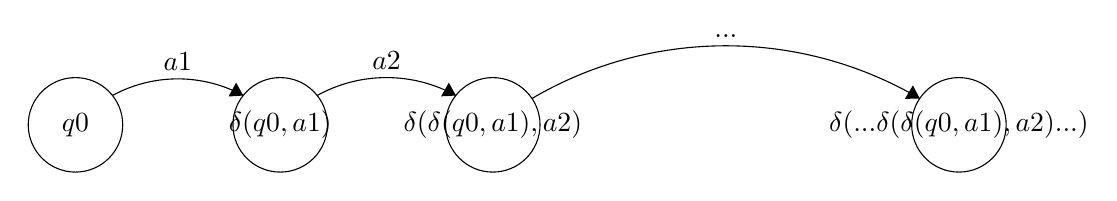
\begin{tikzpicture}[scale=0.2]
\tikzstyle{every node}+=[inner sep=0pt]
\draw [black] (8,-18.2) circle (3);
\draw (8,-18.2) node {$q0$};
\draw [black] (21,-18.2) circle (3);
\draw (21,-18.2) node {$\delta(q0,a1)$};
\draw [black] (34.5,-18.2) circle (3);
\draw (34.5,-18.2) node {$\delta(\delta(q0,a1),a2)$};
\draw [black] (64.1,-18.2) circle (3);
\draw (64.1,-18.2) node {$\delta(...\delta(\delta(q0,a1),a2)...)$};
\draw [black] (10.336,-16.342) arc (118.61376:61.38624:8.694);
\fill [black] (18.66,-16.34) -- (18.2,-15.52) -- (17.72,-16.4);
\draw (14.5,-14.78) node [above] {$a1$};
\draw [black] (23.337,-16.341) arc (119.0469:60.9531:9.089);
\fill [black] (32.16,-16.34) -- (31.71,-15.52) -- (31.22,-16.39);
\draw (27.75,-14.7) node [above] {$a2$};
\draw [black] (36.987,-16.526) arc (120.41027:59.58973:24.325);
\fill [black] (61.61,-16.53) -- (61.18,-15.69) -- (60.67,-16.55);
\draw (49.3,-12.68) node [above] {$...$};
\end{tikzpicture}
\end{center}
\end{definition}

\begin{beispiel}
Berechnung von $A$ auf $w=babbaba$:

\begin{center}
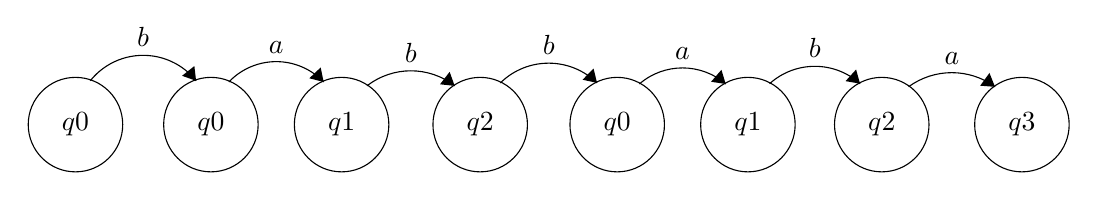
\begin{tikzpicture}[scale=0.2]
\tikzstyle{every node}+=[inner sep=0pt]
\draw [black] (4.7,-18.3) circle (3);
\draw (4.7,-18.3) node {$q0$};
\draw [black] (13.3,-18.3) circle (3);
\draw (13.3,-18.3) node {$q0$};
\draw [black] (21.6,-18.3) circle (3);
\draw (21.6,-18.3) node {$q1$};
\draw [black] (30.4,-18.3) circle (3);
\draw (30.4,-18.3) node {$q2$};
\draw [black] (39.1,-18.3) circle (3);
\draw (39.1,-18.3) node {$q0$};
\draw [black] (47.4,-18.3) circle (3);
\draw (47.4,-18.3) node {$q1$};
\draw [black] (55.9,-18.3) circle (3);
\draw (55.9,-18.3) node {$q2$};
\draw [black] (64.8,-18.3) circle (3);
\draw (64.8,-18.3) node {$q3$};
\draw [black] (5.641,-15.515) arc (-218.64615:-321.35385:4.301);
\fill [black] (12.36,-15.52) -- (12.25,-14.58) -- (11.47,-15.2);
\draw (9,-13.4) node [above] {$b$};
\draw [black] (14.437,-15.594) arc (136.5048:43.4952:4.153);
\fill [black] (20.46,-15.59) -- (20.27,-14.67) -- (19.55,-15.36);
\draw (17.45,-13.8) node [above] {$a$};
\draw [black] (23.215,-15.837) arc (127.82494:52.17506:4.541);
\fill [black] (28.78,-15.84) -- (28.46,-14.95) -- (27.85,-15.74);
\draw (26,-14.38) node [above] {$b$};
\draw [black] (31.682,-15.653) arc (134.51058:45.48942:4.376);
\fill [black] (37.82,-15.65) -- (37.6,-14.74) -- (36.9,-15.45);
\draw (34.75,-13.9) node [above] {$b$};
\draw [black] (40.506,-15.722) arc (130.882:49.118:4.192);
\fill [black] (45.99,-15.72) -- (45.72,-14.82) -- (45.06,-15.58);
\draw (43.25,-14.2) node [above] {$a$};
\draw [black] (48.776,-15.703) arc (132.05645:47.94355:4.291);
\fill [black] (54.52,-15.7) -- (54.27,-14.8) -- (53.6,-15.54);
\draw (51.65,-14.1) node [above] {$b$};
\draw [black] (57.606,-15.896) arc (126.16016:53.83984:4.65);
\fill [black] (63.09,-15.9) -- (62.74,-15.02) -- (62.15,-15.83);
\draw (60.35,-14.5) node [above] {$a$};
\end{tikzpicture}
\end{center}
\end{beispiel}

Sinnvollerweise: Erweiterung von $\delta$ af Wörter (erweiterte Übergangsfunktion).

\begin{definition}[Erweiterte Übergangsfunktion]

$\hat{\delta} : Q \times \Sigma^* \mapsto Q$ ist rekursiv definiert wie folgt:
\begin{itemize}
\item $\hat{\delta}(q,a) = \delta(q,a)$ für alle $q\in Q, a \in \Sigma$
\item $\hat{\delta}(q, xa) = \delta(\hat{\delta}(q, x), a)$ für alle $q \in Q, x \in \Sigma^*, a \in \Sigma$.
\end{itemize}

\end{definition}

\begin{bemerkung}
Anschaulich: $\hat{\delta}(q,w)$ betstimmt, in welchem Zustand $A$ endet, wenn er vom Zustand $q$ aus das Wort $w$ liest.
\end{bemerkung}

\begin{beispiel}
$\hat{\delta}(q_0, babbaba)$
\end{beispiel}

\begin{definition}
Sei $A = (Q, \Sigma, \delta, q_0, F)$ ein DEA. Die von $A$ akzeptierte Sprache $L(A) \subseteq \Sigma^*$ ist die Menge aller $w \in \Sigma^*$, so dass $\hat{\delta}(q_0, w) \in F$.
\end{definition}

\begin{bemerkung}
Anschaulich: Die Menge aller Wörter, die den DEA vom Anfangszustand aus in einen Endzustand führen.
\end{bemerkung}

\begin{beispiel}
$\hat{\delta}(q_0, babbaba) = q_3\in F \Rightarrow w \in L(A)$ ($w$ wird von $A$ akzeptiert.)
\end{beispiel}

\begin{definition}[Reguläre Sprachen]
$\mathcal{L}($DEA$) = \{L(A) | A $ ist ein DEA$ \}$ ist die Klasse der Sprachen, die von DEAs akzeptiert werden. Man nennt sie die Klasse der regulären Sprachen und $L \in \mathcal{L}($DEA$)$ wird regulär genannt.
\end{definition}

\begin{beispiel}
DEA $A$ entwerfen, der die Sprache 
\[L = \{w \in \{0, 1\}^* | w \textrm{ enthält eine gerade Anzahl
Nullen und eine gerade Anzahl Einsen} \}
\]
akzeptiert.

Idee: 4 Zustände, die speichern, wieviele Nullen und Einseln modulo 2 bereits gelesen wurden.

\begin{itemize}
\item $q_{00}$: gerade Anzahl Nullen, gerade Anzahl Einsen
\item $q_{01}$: gerade Anzahl Nullen, ungerade Anzahl Einsen
\item $q_{10}$: ungerade Anzahl Nullen, gerade Anzahl Einsen
\item $q_{11}$: ungerade Anzahl Nullen, ungerade Anzahl Einsen
\end{itemize}

\begin{center}
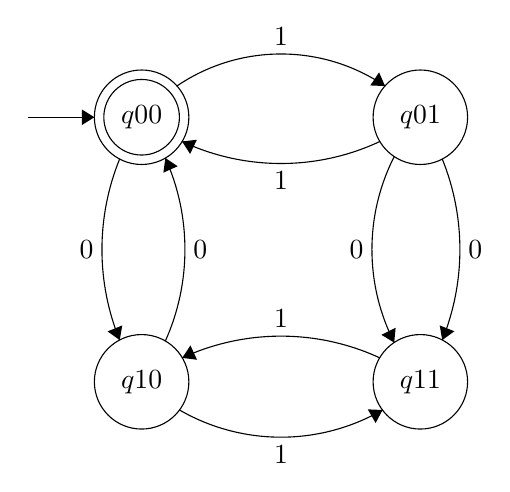
\begin{tikzpicture}[scale=0.2]
\tikzstyle{every node}+=[inner sep=0pt]
\draw [black] (10.7,-14.2) circle (3);
\draw (10.7,-14.2) node {$q00$};
\draw [black] (10.7,-14.2) circle (2.4);
\draw [black] (28.4,-14.2) circle (3);
\draw (28.4,-14.2) node {$q01$};
\draw [black] (10.7,-31) circle (3);
\draw (10.7,-31) node {$q10$};
\draw [black] (28.4,-31) circle (3);
\draw (28.4,-31) node {$q11$};
\draw [black] (3.5,-14.2) -- (7.7,-14.2);
\fill [black] (7.7,-14.2) -- (6.9,-13.7) -- (6.9,-14.7);
\draw [black] (12.94,-12.217) arc (124.21511:55.78489:11.755);
\fill [black] (26.16,-12.22) -- (25.78,-11.35) -- (25.22,-12.18);
\draw (19.55,-9.68) node [above] {$1$};
\draw [black] (25.831,-15.739) arc (-64.89143:-115.10857:14.801);
\fill [black] (13.27,-15.74) -- (13.78,-16.53) -- (14.21,-15.63);
\draw (19.55,-17.64) node [below] {$1$};
\draw [black] (12.207,-16.788) arc (24.16062:-24.16062:14.201);
\fill [black] (12.21,-16.79) -- (12.08,-17.72) -- (12.99,-17.31);
\draw (13.95,-22.6) node [right] {$0$};
\draw [black] (9.305,-28.349) arc (-157.8769:-202.1231:15.267);
\fill [black] (9.31,-28.35) -- (9.47,-27.42) -- (8.54,-27.8);
\draw (7.68,-22.6) node [left] {$0$};
\draw [black] (26.743,-28.507) arc (-153.00161:-206.99839:13.012);
\fill [black] (26.74,-28.51) -- (26.83,-27.57) -- (25.93,-28.02);
\draw (24.83,-22.6) node [left] {$0$};
\draw [black] (29.791,-16.852) arc (22.06226:-22.06226:15.302);
\fill [black] (29.79,-28.35) -- (30.56,-27.79) -- (29.63,-27.42);
\draw (31.41,-22.6) node [right] {$0$};
\draw [black] (25.999,-32.788) arc (-59.99074:-120.00926:12.895);
\fill [black] (26,-32.79) -- (25.06,-32.75) -- (25.56,-33.62);
\draw (19.55,-35.02) node [below] {$1$};
\draw [black] (13.279,-29.478) arc (114.79814:65.20186:14.951);
\fill [black] (13.28,-29.48) -- (14.22,-29.6) -- (13.8,-28.69);
\draw (19.55,-27.6) node [above] {$1$};
\end{tikzpicture}
\end{center}

Tabelle:

\begin{tabular}{r|cc}
 & $0$ & $1$ \\
\hline 
$\mapsto *q_{00}$ & $q_{10}$ & $q_{01}$ \\
$q_{01}$ & $q_{11}$ & $q_{00}$ \\
$q_{10}$ & $q_{00}$ & $q_{11}$ \\
$q_{11}$ & $q_{01}$ & $q_{10}$
\end{tabular}

Berechnung von $A$ auf $w = 011011$:

\begin{center}
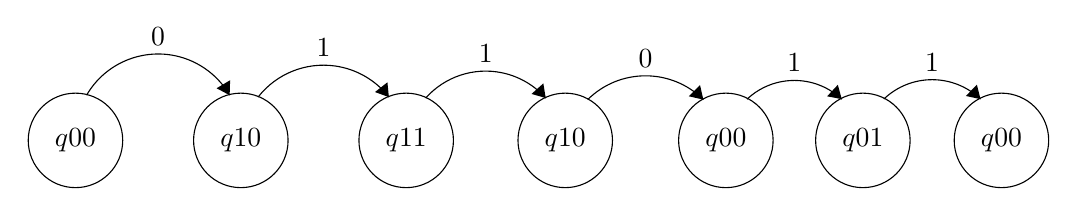
\begin{tikzpicture}[scale=0.2]
\tikzstyle{every node}+=[inner sep=0pt]
\draw [black] (7.6,-19) circle (3);
\draw (7.6,-19) node {$q00$};
\draw [black] (18.1,-19) circle (3);
\draw (18.1,-19) node {$q10$};
\draw [black] (28.6,-19) circle (3);
\draw (28.6,-19) node {$q11$};
\draw [black] (38.7,-19) circle (3);
\draw (38.7,-19) node {$q10$};
\draw [black] (48.9,-19) circle (3);
\draw (48.9,-19) node {$q00$};
\draw [black] (57.6,-19) circle (3);
\draw (57.6,-19) node {$q01$};
\draw [black] (66.4,-19) circle (3);
\draw (66.4,-19) node {$q00$};
\draw [black] (8.307,-16.126) arc (-210.18403:-329.81597:5.255);
\fill [black] (17.39,-16.13) -- (17.42,-15.18) -- (16.56,-15.69);
\draw (12.85,-13.01) node [above] {$0$};
\draw [black] (19.195,-16.25) arc (141.98894:38.01106:5.274);
\fill [black] (27.5,-16.25) -- (27.41,-15.31) -- (26.62,-15.93);
\draw (23.35,-13.72) node [above] {$1$};
\draw [black] (29.837,-16.314) arc (138.41679:41.58321:5.098);
\fill [black] (37.46,-16.31) -- (37.31,-15.38) -- (36.56,-16.05);
\draw (33.65,-14.1) node [above] {$1$};
\draw [black] (40.128,-16.408) arc (134.68822:45.31178:5.222);
\fill [black] (47.47,-16.41) -- (47.26,-15.49) -- (46.55,-16.2);
\draw (43.8,-14.4) node [above] {$0$};
\draw [black] (50.245,-16.383) arc (133.21908:46.78092:4.389);
\fill [black] (56.26,-16.38) -- (56.01,-15.47) -- (55.33,-16.2);
\draw (53.25,-14.69) node [above] {$1$};
\draw [black] (58.932,-16.375) arc (133.72667:46.27333:4.438);
\fill [black] (65.07,-16.38) -- (64.84,-15.46) -- (64.14,-16.18);
\draw (62,-14.64) node [above] {$1$};
\end{tikzpicture}
\end{center}

$\Rightarrow w \in L(A), \hat{\delta}(q_{00},011011) = q_0$

\end{beispiel}

Lösung der Aufgaben

1a:

\begin{center}
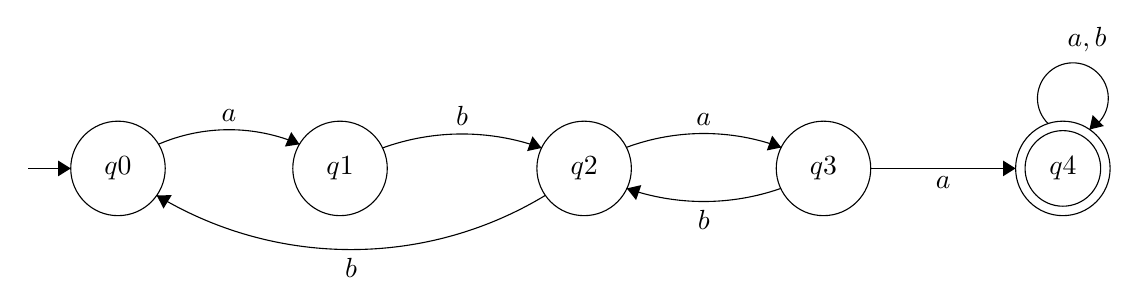
\begin{tikzpicture}[scale=0.2]
\tikzstyle{every node}+=[inner sep=0pt]
\draw [black] (8.6,-18.6) circle (3);
\draw (8.6,-18.6) node {$q0$};
\draw [black] (22.7,-18.6) circle (3);
\draw (22.7,-18.6) node {$q1$};
\draw [black] (38.2,-18.6) circle (3);
\draw (38.2,-18.6) node {$q2$};
\draw [black] (53.4,-18.6) circle (3);
\draw (53.4,-18.6) node {$q3$};
\draw [black] (68.6,-18.6) circle (3);
\draw (68.6,-18.6) node {$q4$};
\draw [black] (68.6,-18.6) circle (2.4);
\draw [black] (2.9,-18.6) -- (5.6,-18.6);
\fill [black] (5.6,-18.6) -- (4.8,-18.1) -- (4.8,-19.1);
\draw [black] (67.67,-15.76) arc (225.8699:-62.1301:2.25);
\draw (70.14,-11.26) node [above] {$a,b$};
\fill [black] (70.29,-16.13) -- (71.2,-15.91) -- (70.49,-15.21);
\draw [black] (56.4,-18.6) -- (65.6,-18.6);
\fill [black] (65.6,-18.6) -- (64.8,-18.1) -- (64.8,-19.1);
\draw (61,-19.1) node [below] {$a$};
\draw [black] (40.881,-17.266) arc (110.36794:69.63206:14.133);
\fill [black] (50.72,-17.27) -- (50.14,-16.52) -- (49.8,-17.46);
\draw (45.8,-15.88) node [above] {$a$};
\draw [black] (50.688,-19.871) arc (-70.70699:-109.29301:14.794);
\fill [black] (40.91,-19.87) -- (41.5,-20.61) -- (41.83,-19.66);
\draw (45.8,-21.2) node [below] {$b$};
\draw [black] (25.398,-17.3) arc (109.92753:70.07247:14.822);
\fill [black] (35.5,-17.3) -- (34.92,-16.56) -- (34.58,-17.5);
\draw (30.45,-15.91) node [above] {$b$};
\draw [black] (11.168,-17.065) arc (113.28858:66.71142:11.338);
\fill [black] (20.13,-17.07) -- (19.6,-16.29) -- (19.2,-17.21);
\draw (15.65,-15.64) node [above] {$a$};
\draw [black] (35.738,-20.311) arc (-58.81659:-121.18341:23.828);
\fill [black] (11.06,-20.31) -- (11.49,-21.15) -- (12.01,-20.3);
\draw (23.4,-24.25) node [below] {$b$};
\end{tikzpicture}
\end{center}

1b:

\begin{center}
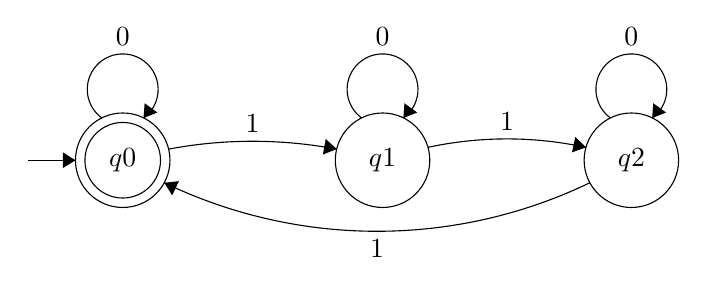
\begin{tikzpicture}[scale=0.2]
\tikzstyle{every node}+=[inner sep=0pt]
\draw [black] (19.6,-18.7) circle (3);
\draw (19.6,-18.7) node {$q0$};
\draw [black] (19.6,-18.7) circle (2.4);
\draw [black] (36.1,-18.7) circle (3);
\draw (36.1,-18.7) node {$q1$};
\draw [black] (51.9,-18.7) circle (3);
\draw (51.9,-18.7) node {$q2$};
\draw [black] (13.6,-18.7) -- (16.6,-18.7);
\fill [black] (16.6,-18.7) -- (15.8,-18.2) -- (15.8,-19.2);
\draw [black] (22.514,-17.993) arc (100.6628:79.3372:28.839);
\fill [black] (33.19,-17.99) -- (32.49,-17.35) -- (32.31,-18.34);
\draw (27.85,-16.99) node [above] {$1$};
\draw [black] (34.777,-16.02) arc (234:-54:2.25);
\draw (36.1,-11.45) node [above] {$0$};
\fill [black] (37.42,-16.02) -- (38.3,-15.67) -- (37.49,-15.08);
\draw [black] (38.984,-17.882) arc (102.20585:77.79415:23.723);
\fill [black] (49.02,-17.88) -- (48.34,-17.22) -- (48.13,-18.2);
\draw (44,-16.85) node [above] {$1$};
\draw [black] (50.577,-16.02) arc (234:-54:2.25);
\draw (51.9,-11.45) node [above] {$0$};
\fill [black] (53.22,-16.02) -- (54.1,-15.67) -- (53.29,-15.08);
\draw [black] (18.277,-16.02) arc (234:-54:2.25);
\draw (19.6,-11.45) node [above] {$0$};
\fill [black] (20.92,-16.02) -- (21.8,-15.67) -- (20.99,-15.08);
\draw [black] (49.264,-20.129) arc (-64.29762:-115.70238:31.159);
\fill [black] (22.24,-20.13) -- (22.74,-20.93) -- (23.17,-20.03);
\draw (35.75,-23.71) node [below] {$1$};
\end{tikzpicture}
\end{center}

\section{Nichtdeterministische erstaunliche Endliche Automaten (NEA)}

Idee: Ein NEA kann sich nach dem Lesen eines Wortes in mehreren Zuständen befinden.

Vorteil: Sie sind einfacher zu entwerfen.

\begin{beispiel}
Akzeptiere alle Wörter, die mit 01 enden.

\begin{center}
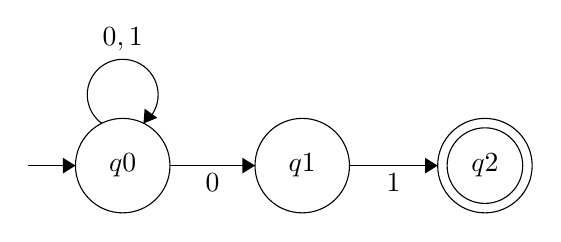
\begin{tikzpicture}[scale=0.2]
\tikzstyle{every node}+=[inner sep=0pt]
\draw [black] (12.3,-18.2) circle (3);
\draw (12.3,-18.2) node {$q0$};
\draw [black] (23.7,-18.2) circle (3);
\draw (23.7,-18.2) node {$q1$};
\draw [black] (35.3,-18.2) circle (3);
\draw (35.3,-18.2) node {$q2$};
\draw [black] (35.3,-18.2) circle (2.4);
\draw [black] (10.977,-15.52) arc (234:-54:2.25);
\draw (12.3,-10.95) node [above] {$0,1$};
\fill [black] (13.62,-15.52) -- (14.5,-15.17) -- (13.69,-14.58);
\draw [black] (6.3,-18.2) -- (9.3,-18.2);
\fill [black] (9.3,-18.2) -- (8.5,-17.7) -- (8.5,-18.7);
\draw [black] (15.3,-18.2) -- (20.7,-18.2);
\fill [black] (20.7,-18.2) -- (19.9,-17.7) -- (19.9,-18.7);
\draw (18,-18.7) node [below] {$0$};
\draw [black] (26.7,-18.2) -- (32.3,-18.2);
\fill [black] (32.3,-18.2) -- (31.5,-17.7) -- (31.5,-18.7);
\draw (29.5,-18.7) node [below] {$1$};
\end{tikzpicture}
\end{center}

Transitionstabelle:

\begin{tabular}{r|cc}
			&	0	&	1	\\
\hline
$\mapsto q_0$	&	$\{q_0,q_1\}$ & $\{q_0\}$		\\
$q_1$		&	$\varnothing$ & $\{q_2\}$	\\
$*q_2$		&	$\varnothing$ & $\varnothing$
\end{tabular}

Mögliche Berenchungen auf dem Wort 00101:

\begin{center}
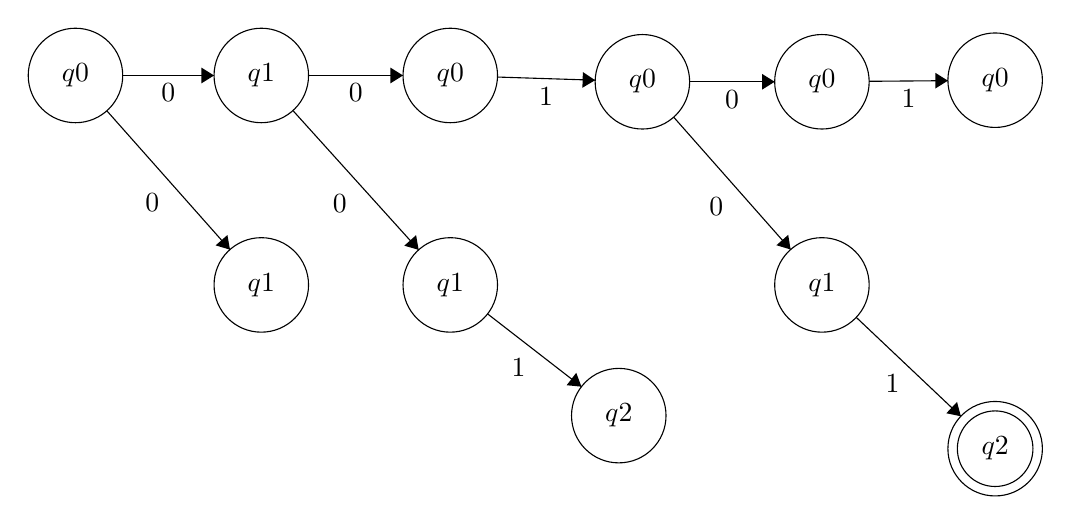
\begin{tikzpicture}[scale=0.2]
\tikzstyle{every node}+=[inner sep=0pt]
\draw [black] (7,-14.7) circle (3);
\draw (7,-14.7) node {$q0$};
\draw [black] (18.8,-14.7) circle (3);
\draw (18.8,-14.7) node {$q1$};
\draw [black] (18.8,-28) circle (3);
\draw (18.8,-28) node {$q1$};
\draw [black] (30.8,-14.7) circle (3);
\draw (30.8,-14.7) node {$q0$};
\draw [black] (30.8,-28) circle (3);
\draw (30.8,-28) node {$q1$};
\draw [black] (43,-15.1) circle (3);
\draw (43,-15.1) node {$q0$};
\draw [black] (41.5,-36.3) circle (3);
\draw (41.5,-36.3) node {$q2$};
\draw [black] (54.4,-15.1) circle (3);
\draw (54.4,-15.1) node {$q0$};
\draw [black] (65.4,-15) circle (3);
\draw (65.4,-15) node {$q0$};
\draw [black] (54.4,-28) circle (3);
\draw (54.4,-28) node {$q1$};
\draw [black] (65.4,-38.4) circle (3);
\draw (65.4,-38.4) node {$q2$};
\draw [black] (65.4,-38.4) circle (2.4);
\draw [black] (10,-14.7) -- (15.8,-14.7);
\fill [black] (15.8,-14.7) -- (15,-14.2) -- (15,-15.2);
\draw (12.9,-15.2) node [below] {$0$};
\draw [black] (8.99,-16.94) -- (16.81,-25.76);
\fill [black] (16.81,-25.76) -- (16.65,-24.83) -- (15.9,-25.49);
\draw (12.36,-22.8) node [left] {$0$};
\draw [black] (21.8,-14.7) -- (27.8,-14.7);
\fill [black] (27.8,-14.7) -- (27,-14.2) -- (27,-15.2);
\draw (24.8,-15.2) node [below] {$0$};
\draw [black] (20.81,-16.93) -- (28.79,-25.77);
\fill [black] (28.79,-25.77) -- (28.63,-24.84) -- (27.88,-25.51);
\draw (24.26,-22.81) node [left] {$0$};
\draw [black] (33.8,-14.8) -- (40,-15);
\fill [black] (40,-15) -- (39.22,-14.48) -- (39.19,-15.48);
\draw (36.88,-15.43) node [below] {$1$};
\draw [black] (33.17,-29.84) -- (39.13,-34.46);
\fill [black] (39.13,-34.46) -- (38.8,-33.58) -- (38.19,-34.37);
\draw (35.14,-32.65) node [below] {$1$};
\draw [black] (46,-15.1) -- (51.4,-15.1);
\fill [black] (51.4,-15.1) -- (50.6,-14.6) -- (50.6,-15.6);
\draw (48.7,-15.6) node [below] {$0$};
\draw [black] (57.4,-15.07) -- (62.4,-15.03);
\fill [black] (62.4,-15.03) -- (61.6,-14.53) -- (61.6,-15.53);
\draw (59.9,-15.56) node [below] {$1$};
\draw [black] (44.99,-17.35) -- (52.41,-25.75);
\fill [black] (52.41,-25.75) -- (52.26,-24.82) -- (51.51,-25.48);
\draw (48.16,-23) node [left] {$0$};
\draw [black] (56.58,-30.06) -- (63.22,-36.34);
\fill [black] (63.22,-36.34) -- (62.98,-35.43) -- (62.3,-36.15);
\draw (58.88,-33.68) node [below] {$1$};
\end{tikzpicture}
\end{center}

\end{beispiel}

\begin{definition}[NEA]
Ein NEA $A$ wird beschrieben durch $A = (Q,\Sigma, \delta, q_0, F)$, wobei
\[
\delta: Q \times \Sigma \mapsto 2^Q = \mathcal{P}(Q)
\]
Die Transitionsfunktion definiert für jeden Zustand und jedes Eingabesymbol eine Menge von Folgezuständen.
\end{definition}

\begin{definition}[Erweiterte NEA-Transitionsfunktion]
Sei $w \in \Sigma^*, q \in Q$. Dann definieren wir
\[
\hat{\delta}: Q \times \Sigma^* \mapsto 2^Q
\]
rekursiv wie folgt:

\begin{itemize}
\item $\hat\delta(q, \varepsilon) = \{ q \}$
\item Sei $w = xa$ und $\hat\delta(q, x) = \{p_1, \dots p_k\}$ für $k \in \mathbb{N}$, dann ist
\[
\hat\delta(q, w) = \bigcup\limits_{i=1}^k \delta(p_i, a)
\]
\end{itemize}
\end{definition}

\begin{beispiel}
\begin{eqnarray*}
\hat\delta(q_0, \varepsilon) &=& \{q_0 \} \textrm{ (Grundregel)} \\
\hat\delta(q_0, 0) = \delta(q_0, 0) &=& \{q_0, q_1 \} \\
\hat\delta(q_0, 00) = \delta(q_0, 0) \cup \delta(q_1, 0) = \{q_0, q_1\} \cup \varnothing &=& \{q_0, q_1\} \\
\hat\delta(q_0, 001) = \delta(q_0, 1) \cup \delta(q_1, 1) = \{q_0\} \cup \{q_2\} &=& \{q_0, q_2\} \\
\hat\delta(q_0, 0010) = \delta(q_0, 0) \cup \delta(q_0, 1) \cup \delta(q_1, 1) = \{q_1\} \cup \{q_2\} &=& \{q_0, q_2\} \textrm{ falsch} \\
\hat\delta(q_0, 00101) = \delta(q_0, 0) \cup \delta(q_0, 1) \cup \delta(q_1, 1) = \{q_1\} \cup \{q_2\} &=& \{q_0, q_2\} \textrm{ falsch}
\end{eqnarray*}
\end{beispiel}

\begin{definition}
Sei $A = (Q, \Sigma, \delta, q_0, F)$ ein NEA. Die von $A$ akzeptierte Sprache $L(A)$ ist $L(A) = \{ w\in \Sigma^* | \hat\delta(q_0, w) \cap F \neq \varnothing\}$, also die Menge aller Wörter, mit denen vom Startzustand aus ein Endzustand erreichbar ist.
\end{definition}

Fragen/Probleme:
\begin{enumerate}
\item Wie kann man möglichst effizient entscheiden, ob ein gegebenes Wort in der Sprache eines gegebenen NEA enthalten ist?
\item Sind NEAs mächtiger als DEAs?
\end{enumerate}

Antwort: DEAs und NEAs sind äquivalent.

Ziel: Automatische Umwandlung von NEAs in DEAs.

\begin{bemerkung}[Teilmengenkonstruktion (Potenzmengenkonstruktion)]
Idee: Zustände des DEA sind Mengen erreichbarer Zustände des NEA.

Formal: Sei $N = (Q_N, \Sigma, \delta_N, q_0, F_N)$ ein NEA. Konstruiere einen äquivalenten DEA $D = (Q_D, \Sigma, \delta_D, \{q_0\}, F_D)$ mit
\begin{itemize}
\item $Q_D = 2^{Q_N}$
\item $F = \{S \subseteq Q_D | S\cap F \neq \varnothing \}$
\item $\delta_D(S, a) = \bigcup\limits_{p \in S} \delta_N(p, a)$ für $S \in Q_D, a \in \Sigma$
\end{itemize}
\end{bemerkung}

\begin{beispiel}[von vorher]
Konstruktion des äquivalenten DEAs als Übergangstabelle.

\begin{tabular}{rl|ll}
&& 0 & 1\\
\hline
A&$\varnothing$ & $\varnothing = A$ & $\varnothing = A$   \\
B&$\mapsto\{q_0\}$ & $\{q_0, q_1\} = E$ & $\{q_0\} = B$ \\
C&$\{q_1\}$ & $\varnothing = A$ & $\{q_2\} = D$ \\
D&$*\{q_2\}$ & $\varnothing$ & $\varnothing$ \\
E&$\{q_0, q_1\}$ & $\{q_0, q_1\}$ & $\{q_0, q_2\}$ \\
F&$*\{q_0, q_2\}$ & $\{q_0,q_1\}$ & $\{q_0\}$ \\
G&$*\{q_1, q_2\}$ & $\varnothing$ & $\{q_2\}$ \\
H&$*\{q_1, q_2, q_3\}$ & $\{q_0, q_1\}$ & $\{q_0,q_2\}$ \\
\end{tabular}

\begin{center}
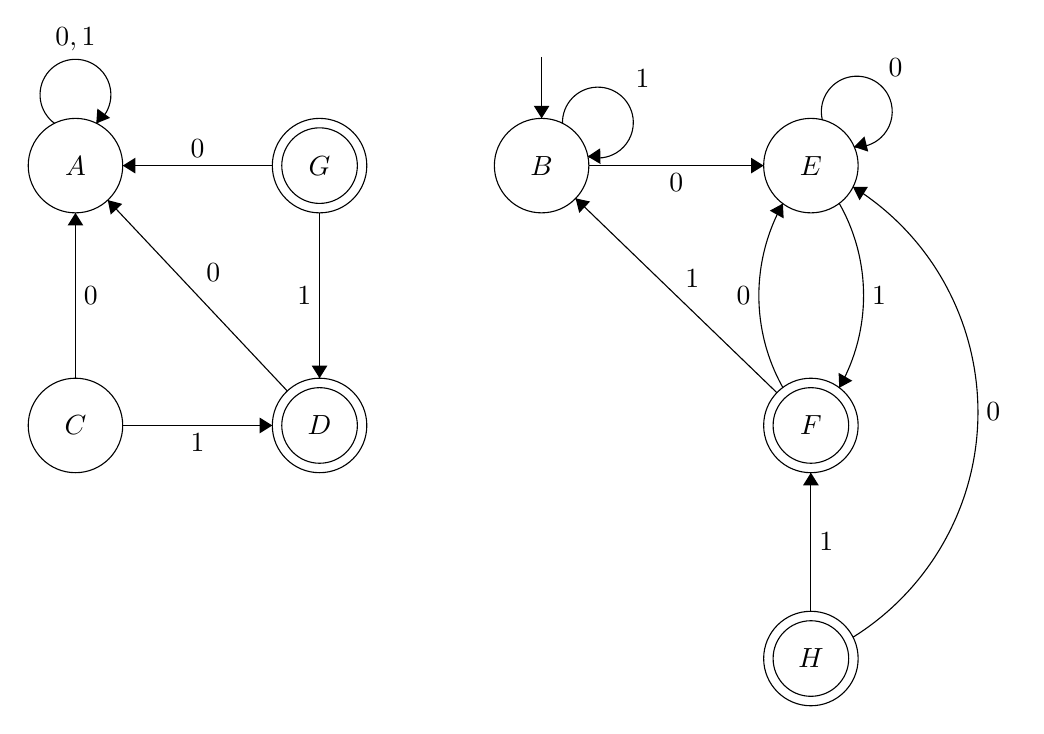
\begin{tikzpicture}[scale=0.2]
\tikzstyle{every node}+=[inner sep=0pt]
\draw [black] (11.6,-12.4) circle (3);
\draw (11.6,-12.4) node {$A$};
\draw [black] (27.1,-12.4) circle (3);
\draw (27.1,-12.4) node {$G$};
\draw [black] (27.1,-12.4) circle (2.4);
\draw [black] (41.2,-12.4) circle (3);
\draw (41.2,-12.4) node {$B$};
\draw [black] (58.3,-12.4) circle (3);
\draw (58.3,-12.4) node {$E$};
\draw [black] (11.6,-28.9) circle (3);
\draw (11.6,-28.9) node {$C$};
\draw [black] (27.1,-28.9) circle (3);
\draw (27.1,-28.9) node {$D$};
\draw [black] (27.1,-28.9) circle (2.4);
\draw [black] (58.3,-28.9) circle (3);
\draw (58.3,-28.9) node {$F$};
\draw [black] (58.3,-28.9) circle (2.4);
\draw [black] (58.3,-43.7) circle (3);
\draw (58.3,-43.7) node {$H$};
\draw [black] (58.3,-43.7) circle (2.4);
\draw [black] (41.2,-5.5) -- (41.2,-9.4);
\fill [black] (41.2,-9.4) -- (41.7,-8.6) -- (40.7,-8.6);
\draw [black] (10.277,-9.72) arc (234:-54:2.25);
\draw (11.6,-5.15) node [above] {$0,1$};
\fill [black] (12.92,-9.72) -- (13.8,-9.37) -- (12.99,-8.78);
\draw [black] (42.525,-9.722) arc (181.40536:-106.59464:2.25);
\draw (47.13,-6.89) node [right] {$1$};
\fill [black] (44.13,-11.82) -- (44.94,-12.3) -- (44.92,-11.3);
\draw [black] (44.2,-12.4) -- (55.3,-12.4);
\fill [black] (55.3,-12.4) -- (54.5,-11.9) -- (54.5,-12.9);
\draw (49.75,-12.9) node [below] {$0$};
\draw [black] (14.6,-28.9) -- (24.1,-28.9);
\fill [black] (24.1,-28.9) -- (23.3,-28.4) -- (23.3,-29.4);
\draw (19.35,-29.4) node [below] {$1$};
\draw [black] (11.6,-25.9) -- (11.6,-15.4);
\fill [black] (11.6,-15.4) -- (11.1,-16.2) -- (12.1,-16.2);
\draw (12.1,-20.65) node [right] {$0$};
\draw [black] (25.05,-26.71) -- (13.65,-14.59);
\fill [black] (13.65,-14.59) -- (13.84,-15.51) -- (14.57,-14.83);
\draw (19.88,-19.18) node [right] {$0$};
\draw [black] (59.028,-9.502) arc (193.63546:-94.36454:2.25);
\draw (63.68,-6.77) node [above] {$0$};
\fill [black] (61.04,-11.21) -- (61.94,-11.51) -- (61.7,-10.54);
\draw [black] (60.096,-14.793) arc (29.63396:-29.63396:11.845);
\fill [black] (60.1,-26.51) -- (60.93,-26.06) -- (60.06,-25.56);
\draw (62.15,-20.65) node [right] {$1$};
\draw [black] (56.521,-26.494) arc (-150.7208:-209.2792:11.949);
\fill [black] (56.52,-14.81) -- (55.69,-15.26) -- (56.57,-15.75);
\draw (54.49,-20.65) node [left] {$0$};
\draw [black] (56.14,-26.82) -- (43.36,-14.48);
\fill [black] (43.36,-14.48) -- (43.59,-15.4) -- (44.28,-14.68);
\draw (50.77,-20.17) node [above] {$1$};
\draw [black] (24.1,-12.4) -- (14.6,-12.4);
\fill [black] (14.6,-12.4) -- (15.4,-12.9) -- (15.4,-11.9);
\draw (19.35,-11.9) node [above] {$0$};
\draw [black] (27.1,-15.4) -- (27.1,-25.9);
\fill [black] (27.1,-25.9) -- (27.6,-25.1) -- (26.6,-25.1);
\draw (26.6,-20.65) node [left] {$1$};
\draw [black] (60.973,-13.753) arc (58.05062:-58.05062:16.849);
\fill [black] (60.97,-13.75) -- (61.39,-14.6) -- (61.92,-13.75);
\draw (69.41,-28.05) node [right] {$0$};
\draw [black] (58.3,-40.7) -- (58.3,-31.9);
\fill [black] (58.3,-31.9) -- (57.8,-32.7) -- (58.8,-32.7);
\draw (58.8,-36.3) node [right] {$1$};
\end{tikzpicture}
\end{center}

Der linke Teil ist nicht erreichbar:

\begin{center}
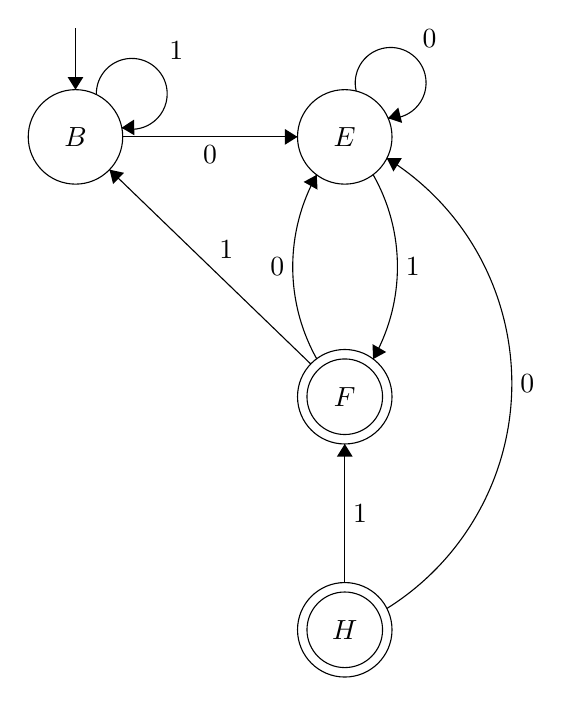
\begin{tikzpicture}[scale=0.2]
\tikzstyle{every node}+=[inner sep=0pt]
\draw [black] (41.2,-12.4) circle (3);
\draw (41.2,-12.4) node {$B$};
\draw [black] (58.3,-12.4) circle (3);
\draw (58.3,-12.4) node {$E$};
\draw [black] (58.3,-28.9) circle (3);
\draw (58.3,-28.9) node {$F$};
\draw [black] (58.3,-28.9) circle (2.4);
\draw [black] (58.3,-43.7) circle (3);
\draw (58.3,-43.7) node {$H$};
\draw [black] (58.3,-43.7) circle (2.4);
\draw [black] (41.2,-5.5) -- (41.2,-9.4);
\fill [black] (41.2,-9.4) -- (41.7,-8.6) -- (40.7,-8.6);
\draw [black] (42.525,-9.722) arc (181.40536:-106.59464:2.25);
\draw (47.13,-6.89) node [right] {$1$};
\fill [black] (44.13,-11.82) -- (44.94,-12.3) -- (44.92,-11.3);
\draw [black] (44.2,-12.4) -- (55.3,-12.4);
\fill [black] (55.3,-12.4) -- (54.5,-11.9) -- (54.5,-12.9);
\draw (49.75,-12.9) node [below] {$0$};
\draw [black] (59.028,-9.502) arc (193.63546:-94.36454:2.25);
\draw (63.68,-6.77) node [above] {$0$};
\fill [black] (61.04,-11.21) -- (61.94,-11.51) -- (61.7,-10.54);
\draw [black] (60.096,-14.793) arc (29.63396:-29.63396:11.845);
\fill [black] (60.1,-26.51) -- (60.93,-26.06) -- (60.06,-25.56);
\draw (62.15,-20.65) node [right] {$1$};
\draw [black] (56.521,-26.494) arc (-150.7208:-209.2792:11.949);
\fill [black] (56.52,-14.81) -- (55.69,-15.26) -- (56.57,-15.75);
\draw (54.49,-20.65) node [left] {$0$};
\draw [black] (56.14,-26.82) -- (43.36,-14.48);
\fill [black] (43.36,-14.48) -- (43.59,-15.4) -- (44.28,-14.68);
\draw (50.77,-20.17) node [above] {$1$};
\draw [black] (60.973,-13.753) arc (58.05062:-58.05062:16.849);
\fill [black] (60.97,-13.75) -- (61.39,-14.6) -- (61.92,-13.75);
\draw (69.41,-28.05) node [right] {$0$};
\draw [black] (58.3,-40.7) -- (58.3,-31.9);
\fill [black] (58.3,-31.9) -- (57.8,-32.7) -- (58.8,-32.7);
\draw (58.8,-36.3) node [right] {$1$};
\end{tikzpicture}
\end{center}

$H$ ist ebenfalls nicht erreichbar:

\begin{center}
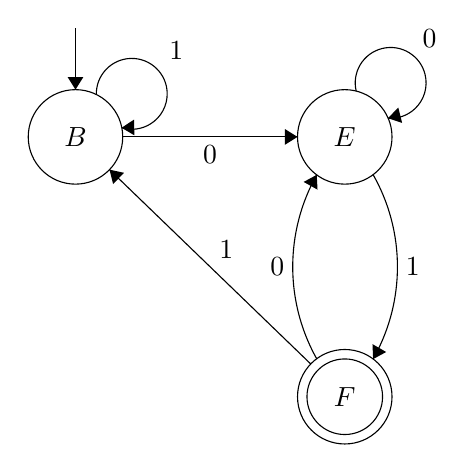
\begin{tikzpicture}[scale=0.2]
\tikzstyle{every node}+=[inner sep=0pt]
\draw [black] (41.2,-12.4) circle (3);
\draw (41.2,-12.4) node {$B$};
\draw [black] (58.3,-12.4) circle (3);
\draw (58.3,-12.4) node {$E$};
\draw [black] (58.3,-28.9) circle (3);
\draw (58.3,-28.9) node {$F$};
\draw [black] (58.3,-28.9) circle (2.4);
\draw [black] (41.2,-5.5) -- (41.2,-9.4);
\fill [black] (41.2,-9.4) -- (41.7,-8.6) -- (40.7,-8.6);
\draw [black] (42.525,-9.722) arc (181.40536:-106.59464:2.25);
\draw (47.13,-6.89) node [right] {$1$};
\fill [black] (44.13,-11.82) -- (44.94,-12.3) -- (44.92,-11.3);
\draw [black] (44.2,-12.4) -- (55.3,-12.4);
\fill [black] (55.3,-12.4) -- (54.5,-11.9) -- (54.5,-12.9);
\draw (49.75,-12.9) node [below] {$0$};
\draw [black] (59.028,-9.502) arc (193.63546:-94.36454:2.25);
\draw (63.68,-6.77) node [above] {$0$};
\fill [black] (61.04,-11.21) -- (61.94,-11.51) -- (61.7,-10.54);
\draw [black] (60.096,-14.793) arc (29.63396:-29.63396:11.845);
\fill [black] (60.1,-26.51) -- (60.93,-26.06) -- (60.06,-25.56);
\draw (62.15,-20.65) node [right] {$1$};
\draw [black] (56.521,-26.494) arc (-150.7208:-209.2792:11.949);
\fill [black] (56.52,-14.81) -- (55.69,-15.26) -- (56.57,-15.75);
\draw (54.49,-20.65) node [left] {$0$};
\draw [black] (56.14,-26.82) -- (43.36,-14.48);
\fill [black] (43.36,-14.48) -- (43.59,-15.4) -- (44.28,-14.68);
\draw (50.77,-20.17) node [above] {$1$};
\end{tikzpicture}
\end{center}

\end{beispiel}

\begin{beispiel}[Ein ungünstiger Fall für die Teilmengenkonstruktion]

\begin{eqnarray*}
L_n &=& \{w \in \{0,1\}^* | \textrm{ Das $n$-t-letzte Zeichen von $w$ ist eine 1} \} \\
&=& \{w \in \{0,1\}^* | w = x1y \textrm{ mit } x \in \{0,1\}^*, y \in \{0,1\}^{n-1} \} \\
\end{eqnarray*}

NEA für $L_n$ mit $n+1$ Zuständen:

\begin{center}
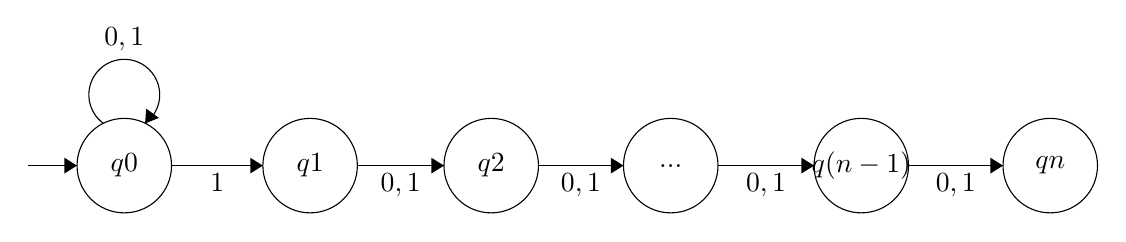
\begin{tikzpicture}[scale=0.2]
\tikzstyle{every node}+=[inner sep=0pt]
\draw [black] (8.4,-16.9) circle (3);
\draw (8.4,-16.9) node {$q0$};
\draw [black] (20.2,-16.9) circle (3);
\draw (20.2,-16.9) node {$q1$};
\draw [black] (31.7,-16.9) circle (3);
\draw (31.7,-16.9) node {$q2$};
\draw [black] (43.1,-16.9) circle (3);
\draw (43.1,-16.9) node {$...$};
\draw [black] (55.2,-16.9) circle (3);
\draw (55.2,-16.9) node {$q(n-1)$};
\draw [black] (67.2,-16.9) circle (3);
\draw (67.2,-16.9) node {$qn$};
\draw [black] (2.3,-16.9) -- (5.4,-16.9);
\fill [black] (5.4,-16.9) -- (4.6,-16.4) -- (4.6,-17.4);
\draw [black] (7.077,-14.22) arc (234:-54:2.25);
\draw (8.4,-9.65) node [above] {$0,1$};
\fill [black] (9.72,-14.22) -- (10.6,-13.87) -- (9.79,-13.28);
\draw [black] (11.4,-16.9) -- (17.2,-16.9);
\fill [black] (17.2,-16.9) -- (16.4,-16.4) -- (16.4,-17.4);
\draw (14.3,-17.4) node [below] {$1$};
\draw [black] (23.2,-16.9) -- (28.7,-16.9);
\fill [black] (28.7,-16.9) -- (27.9,-16.4) -- (27.9,-17.4);
\draw (25.95,-17.4) node [below] {$0,1$};
\draw [black] (34.7,-16.9) -- (40.1,-16.9);
\fill [black] (40.1,-16.9) -- (39.3,-16.4) -- (39.3,-17.4);
\draw (37.4,-17.4) node [below] {$0,1$};
\draw [black] (46.1,-16.9) -- (52.2,-16.9);
\fill [black] (52.2,-16.9) -- (51.4,-16.4) -- (51.4,-17.4);
\draw (49.15,-17.4) node [below] {$0,1$};
\draw [black] (58.2,-16.9) -- (64.2,-16.9);
\fill [black] (64.2,-16.9) -- (63.4,-16.4) -- (63.4,-17.4);
\draw (61.2,-17.4) node [below] {$0,1$};
\end{tikzpicture}
\end{center}

Aber jeder DEA für $L_n$ braucht mindestens $2^n$ Zustände, weil der DEA sich an die letzten $n$ gelesenen Symbole erinnern muss, da er nicht weiss, wann das Wortende kommt. D.h. $2^n$ verschiedene Teilworte mpssen unterscheiden werden. D.h. $2^n$ Zustände nötig.

Beispiel mit $n = 2$:

\begin{center}
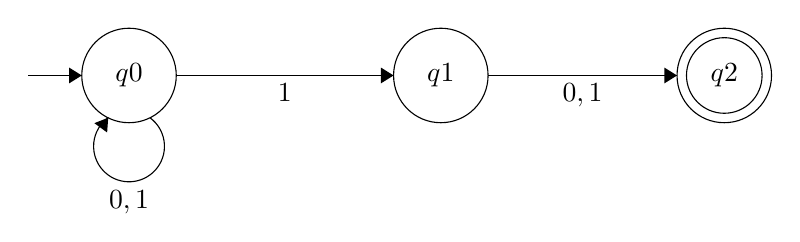
\begin{tikzpicture}[scale=0.2]
\tikzstyle{every node}+=[inner sep=0pt]
\draw [black] (10.1,-10) circle (3);
\draw (10.1,-10) node {$q0$};
\draw [black] (29.9,-10) circle (3);
\draw (29.9,-10) node {$q1$};
\draw [black] (47.9,-10) circle (3);
\draw (47.9,-10) node {$q2$};
\draw [black] (47.9,-10) circle (2.4);
\draw [black] (3.7,-10) -- (7.1,-10);
\fill [black] (7.1,-10) -- (6.3,-9.5) -- (6.3,-10.5);
\draw [black] (13.1,-10) -- (26.9,-10);
\fill [black] (26.9,-10) -- (26.1,-9.5) -- (26.1,-10.5);
\draw (20,-10.5) node [below] {$1$};
\draw [black] (32.9,-10) -- (44.9,-10);
\fill [black] (44.9,-10) -- (44.1,-9.5) -- (44.1,-10.5);
\draw (38.9,-10.5) node [below] {$0,1$};
\draw [black] (11.423,-12.68) arc (54:-234:2.25);
\draw (10.1,-17.25) node [below] {$0,1$};
\fill [black] (8.78,-12.68) -- (7.9,-13.03) -- (8.71,-13.62);
\end{tikzpicture}
\end{center}


\end{beispiel}

\begin{beispiel}[Lösung der Knobelaufgabe]
Wir machen uns zunutze:
\[
2^k \mod 3 = \begin{cases}
1 \textrm{ falls $k$ gerade}\\
1 \textrm{ falls $k$ gerade}
\end{cases}
\]
Wir haben Zustände $q_{ij}$. $i$ ist der Exponent der nächsten 2er-Potenz modulo 2, $j$ ist die Teilsumme.

\begin{center}
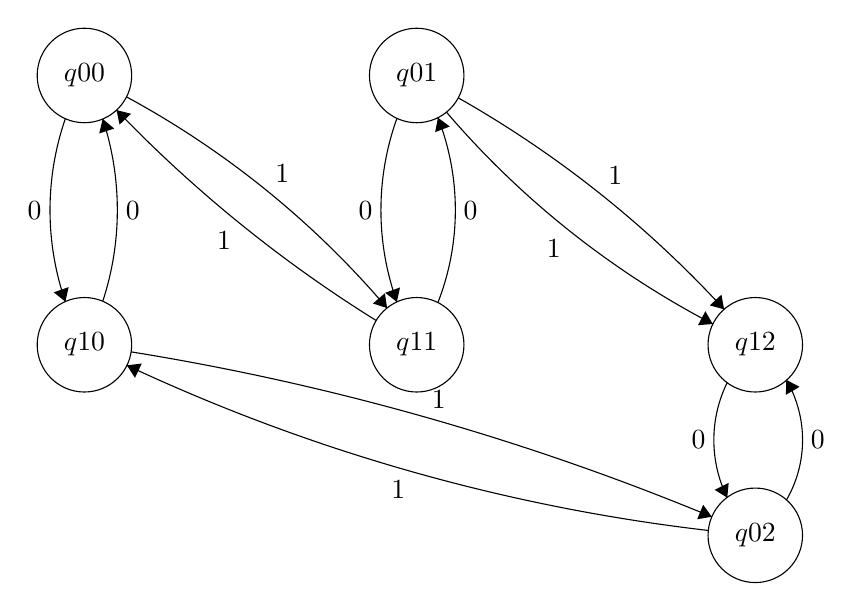
\begin{tikzpicture}[scale=0.2]
\tikzstyle{every node}+=[inner sep=0pt]
\draw [black] (12.3,-12.3) circle (3);
\draw (12.3,-12.3) node {$q00$};
\draw [black] (33.4,-12.3) circle (3);
\draw (33.4,-12.3) node {$q01$};
\draw [black] (54.9,-41.5) circle (3);
\draw (54.9,-41.5) node {$q02$};
\draw [black] (12.3,-29.4) circle (3);
\draw (12.3,-29.4) node {$q10$};
\draw [black] (33.4,-29.4) circle (3);
\draw (33.4,-29.4) node {$q11$};
\draw [black] (54.9,-29.4) circle (3);
\draw (54.9,-29.4) node {$q12$};
\draw [black] (11.088,-26.66) arc (-160.96425:-199.03575:17.812);
\fill [black] (11.09,-26.66) -- (11.3,-25.74) -- (10.35,-26.07);
\draw (9.61,-20.85) node [left] {$0$};
\draw [black] (32.144,-26.68) arc (-160.21504:-199.78496:17.222);
\fill [black] (32.14,-26.68) -- (32.34,-25.76) -- (31.4,-26.1);
\draw (30.63,-20.85) node [left] {$0$};
\draw [black] (13.463,-15.062) arc (18.20228:-18.20228:18.53);
\fill [black] (13.46,-15.06) -- (13.24,-15.98) -- (14.19,-15.67);
\draw (14.89,-20.85) node [right] {$0$};
\draw [black] (34.746,-14.976) arc (21.36604:-21.36604:16.122);
\fill [black] (34.75,-14.98) -- (34.57,-15.9) -- (35.5,-15.54);
\draw (36.35,-20.85) node [right] {$0$};
\draw [black] (56.874,-31.634) arc (30.15203:-30.15203:7.598);
\fill [black] (56.87,-31.63) -- (56.84,-32.58) -- (57.71,-32.07);
\draw (58.4,-35.45) node [right] {$0$};
\draw [black] (53.12,-39.106) arc (-153.76161:-206.23839:8.269);
\fill [black] (53.12,-39.11) -- (53.21,-38.17) -- (52.32,-38.61);
\draw (51.77,-35.45) node [left] {$0$};
\draw [black] (14.974,-13.66) arc (61.55554:40.40001:57.995);
\fill [black] (31.52,-27.07) -- (31.38,-26.13) -- (30.62,-26.78);
\draw (24.87,-19.1) node [above] {$1$};
\draw [black] (30.826,-27.86) arc (-121.90133:-136.14312:85.589);
\fill [black] (14.34,-14.5) -- (14.53,-15.42) -- (15.26,-14.73);
\draw (21.16,-22.19) node [below] {$1$};
\draw [black] (36.041,-13.722) arc (60.45451:42.5516:69.301);
\fill [black] (52.92,-27.15) -- (52.75,-26.22) -- (52.01,-26.9);
\draw (46.01,-19.28) node [above] {$1$};
\draw [black] (52.205,-28.083) arc (-117.55558:-139.43831:56.935);
\fill [black] (52.2,-28.08) -- (51.73,-27.27) -- (51.26,-28.16);
\draw (42.1,-22.66) node [below] {$1$};
\draw [black] (15.266,-29.851) arc (80.83065:67.45627:164.59);
\fill [black] (52.14,-40.32) -- (51.59,-39.56) -- (51.21,-40.48);
\draw (34.81,-33.46) node [above] {$1$};
\draw [black] (51.916,-41.192) arc (-96.61786:-115.09522:119.515);
\fill [black] (15,-30.71) -- (15.51,-31.5) -- (15.94,-30.59);
\draw (32.23,-38) node [below] {$1$};
\end{tikzpicture}
\end{center}

\end{beispiel}

\section{NEAs mit $\varepsilon$-Übergängen}

\begin{center}
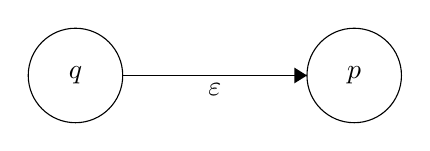
\begin{tikzpicture}[scale=0.2]
\tikzstyle{every node}+=[inner sep=0pt]
\draw [black] (25.6,-25) circle (3);
\draw (25.6,-25) node {$q$};
\draw [black] (43.3,-25) circle (3);
\draw (43.3,-25) node {$p$};
\draw [black] (28.6,-25) -- (40.3,-25);
\fill [black] (40.3,-25) -- (39.5,-24.5) -- (39.5,-25.5);
\draw (34.45,-25.5) node [below] {$\varepsilon$};
\end{tikzpicture}
\end{center}


\begin{beispiel}
Suche nach mehreren Mustern. $L = \{w \in \{ a,b \}^* | \textrm{ enthält eines der Teilwörter aba, abb, bab } \}$ Der NEA $N$ mit $L(N) = L$ mit $\varepsilon$-Übergängen sieht aus:

\begin{center}
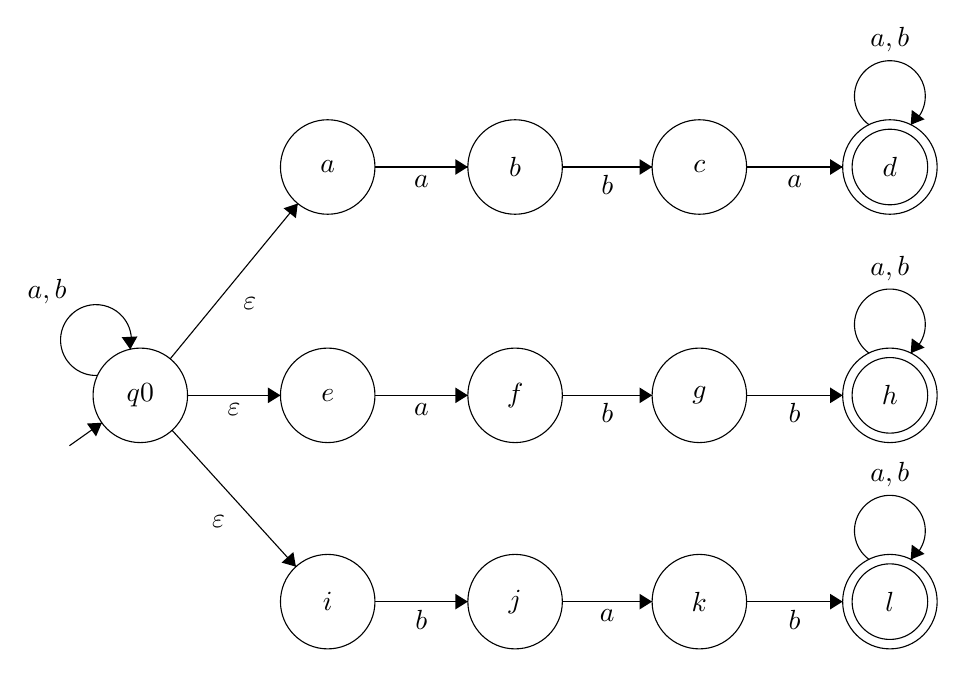
\begin{tikzpicture}[scale=0.2]
\tikzstyle{every node}+=[inner sep=0pt]
\draw [black] (9.4,-24.3) circle (3);
\draw (9.4,-24.3) node {$q0$};
\draw [black] (21.3,-9.8) circle (3);
\draw (21.3,-9.8) node {$a$};
\draw [black] (33.2,-9.8) circle (3);
\draw (33.2,-9.8) node {$b$};
\draw [black] (44.9,-9.8) circle (3);
\draw (44.9,-9.8) node {$c$};
\draw [black] (57,-9.8) circle (3);
\draw (57,-9.8) node {$d$};
\draw [black] (57,-9.8) circle (2.4);
\draw [black] (21.3,-24.3) circle (3);
\draw (21.3,-24.3) node {$e$};
\draw [black] (33.2,-24.3) circle (3);
\draw (33.2,-24.3) node {$f$};
\draw [black] (44.9,-24.3) circle (3);
\draw (44.9,-24.3) node {$g$};
\draw [black] (57,-24.3) circle (3);
\draw (57,-24.3) node {$h$};
\draw [black] (57,-24.3) circle (2.4);
\draw [black] (21.3,-37.4) circle (3);
\draw (21.3,-37.4) node {$i$};
\draw [black] (33.2,-37.4) circle (3);
\draw (33.2,-37.4) node {$j$};
\draw [black] (44.9,-37.4) circle (3);
\draw (44.9,-37.4) node {$k$};
\draw [black] (57,-37.4) circle (3);
\draw (57,-37.4) node {$l$};
\draw [black] (57,-37.4) circle (2.4);
\draw [black] (4.9,-27.5) -- (6.96,-26.04);
\fill [black] (6.96,-26.04) -- (6.01,-26.09) -- (6.59,-26.91);
\draw [black] (6.692,-23.036) arc (272.71751:-15.28249:2.25);
\draw (3.48,-18.54) node [above] {$a,b$};
\fill [black] (8.76,-21.38) -- (9.22,-20.56) -- (8.22,-20.61);
\draw [black] (55.677,-7.12) arc (234:-54:2.25);
\draw (57,-2.55) node [above] {$a,b$};
\fill [black] (58.32,-7.12) -- (59.2,-6.77) -- (58.39,-6.18);
\draw [black] (11.3,-21.98) -- (19.4,-12.12);
\fill [black] (19.4,-12.12) -- (18.5,-12.42) -- (19.28,-13.05);
\draw (15.91,-18.48) node [right] {$\varepsilon$};
\draw [black] (24.3,-9.8) -- (30.2,-9.8);
\fill [black] (30.2,-9.8) -- (29.4,-9.3) -- (29.4,-10.3);
\draw (27.25,-10.3) node [below] {$a$};
\draw [black] (36.2,-9.8) -- (41.9,-9.8);
\fill [black] (41.9,-9.8) -- (41.1,-9.3) -- (41.1,-10.3);
\draw (39.05,-10.3) node [below] {$b$};
\draw [black] (47.9,-9.8) -- (54,-9.8);
\fill [black] (54,-9.8) -- (53.2,-9.3) -- (53.2,-10.3);
\draw (50.95,-10.3) node [below] {$a$};
\draw [black] (12.4,-24.3) -- (18.3,-24.3);
\fill [black] (18.3,-24.3) -- (17.5,-23.8) -- (17.5,-24.8);
\draw (15.35,-24.8) node [below] {$\varepsilon$};
\draw [black] (24.3,-24.3) -- (30.2,-24.3);
\fill [black] (30.2,-24.3) -- (29.4,-23.8) -- (29.4,-24.8);
\draw (27.25,-24.8) node [below] {$a$};
\draw [black] (36.2,-24.3) -- (41.9,-24.3);
\fill [black] (41.9,-24.3) -- (41.1,-23.8) -- (41.1,-24.8);
\draw (39.05,-24.8) node [below] {$b$};
\draw [black] (47.9,-24.3) -- (54,-24.3);
\fill [black] (54,-24.3) -- (53.2,-23.8) -- (53.2,-24.8);
\draw (50.95,-24.8) node [below] {$b$};
\draw [black] (11.42,-26.52) -- (19.28,-35.18);
\fill [black] (19.28,-35.18) -- (19.12,-34.25) -- (18.37,-34.92);
\draw (14.81,-32.31) node [left] {$\varepsilon$};
\draw [black] (24.3,-37.4) -- (30.2,-37.4);
\fill [black] (30.2,-37.4) -- (29.4,-36.9) -- (29.4,-37.9);
\draw (27.25,-37.9) node [below] {$b$};
\draw [black] (36.2,-37.4) -- (41.9,-37.4);
\fill [black] (41.9,-37.4) -- (41.1,-36.9) -- (41.1,-37.9);
\draw (39.05,-37.9) node [below] {$a$};
\draw [black] (47.9,-37.4) -- (54,-37.4);
\fill [black] (54,-37.4) -- (53.2,-36.9) -- (53.2,-37.9);
\draw (50.95,-37.9) node [below] {$b$};
\draw [black] (55.677,-21.62) arc (234:-54:2.25);
\draw (57,-17.05) node [above] {$a,b$};
\fill [black] (58.32,-21.62) -- (59.2,-21.27) -- (58.39,-20.68);
\draw [black] (55.677,-34.72) arc (234:-54:2.25);
\draw (57,-30.15) node [above] {$a,b$};
\fill [black] (58.32,-34.72) -- (59.2,-34.37) -- (58.39,-33.78);
\end{tikzpicture}
\end{center}

\end{beispiel}

\begin{beispiel}
Ein $\varepsilon$-NEA, der Dezimalzahlen akzeptiert, die sich zusammensetzen aus:
\begin{itemize}
\item optionales $+$ oder $-$
\item Zeichenreihe von Ziffern
\item Dezimalpunkt
\item Zeichenreihe von Ziffern
\end{itemize}
Eine der beiden Zeichenreihen von Ziffern darf leer sein.

Der Automat $E$ sieht dann so aus:
\begin{center}
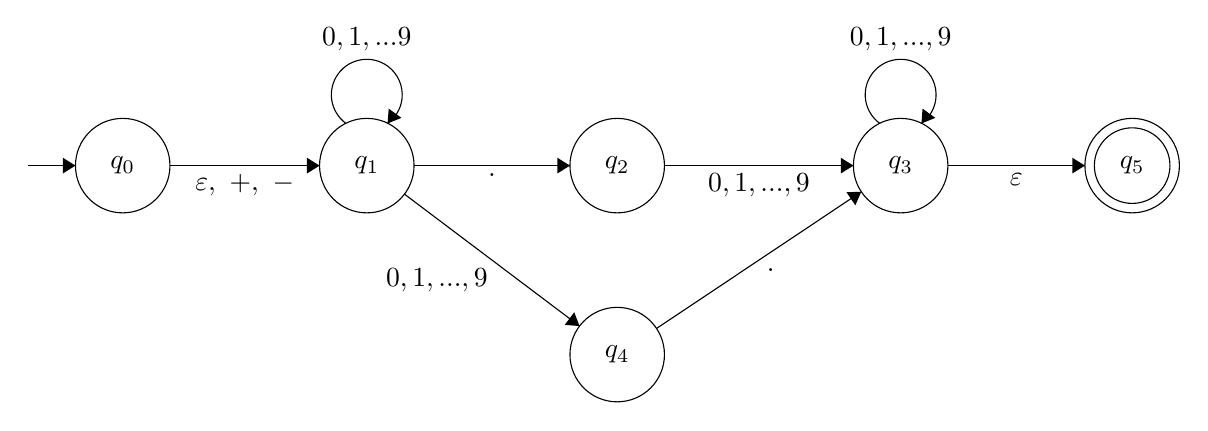
\begin{tikzpicture}[scale=0.2]
\tikzstyle{every node}+=[inner sep=0pt]
\draw [black] (10.1,-15.1) circle (3);
\draw (10.1,-15.1) node {$q_0$};
\draw [black] (25.6,-15.1) circle (3);
\draw (25.6,-15.1) node {$q_1$};
\draw [black] (41.5,-15.1) circle (3);
\draw (41.5,-15.1) node {$q_2$};
\draw [black] (59.5,-15.1) circle (3);
\draw (59.5,-15.1) node {$q_3$};
\draw [black] (74.2,-15.1) circle (3);
\draw (74.2,-15.1) node {$q_5$};
\draw [black] (74.2,-15.1) circle (2.4);
\draw [black] (41.5,-27.1) circle (3);
\draw (41.5,-27.1) node {$q_4$};
\draw [black] (4.1,-15.1) -- (7.1,-15.1);
\fill [black] (7.1,-15.1) -- (6.3,-14.6) -- (6.3,-15.6);
\draw [black] (13.1,-15.1) -- (22.6,-15.1);
\fill [black] (22.6,-15.1) -- (21.8,-14.6) -- (21.8,-15.6);
\draw (17.85,-15.6) node [below] {$\varepsilon,\mbox{ }+,\mbox{ }-$};
\draw [black] (24.277,-12.42) arc (234:-54:2.25);
\draw (25.6,-7.85) node [above] {$0,1,...9$};
\fill [black] (26.92,-12.42) -- (27.8,-12.07) -- (26.99,-11.48);
\draw [black] (28.6,-15.1) -- (38.5,-15.1);
\fill [black] (38.5,-15.1) -- (37.7,-14.6) -- (37.7,-15.6);
\draw (33.55,-15.6) node [below] {$.$};
\draw [black] (44.5,-15.1) -- (56.5,-15.1);
\fill [black] (56.5,-15.1) -- (55.7,-14.6) -- (55.7,-15.6);
\draw (50.5,-15.6) node [below] {$0,1,...,9$};
\draw [black] (62.5,-15.1) -- (71.2,-15.1);
\fill [black] (71.2,-15.1) -- (70.4,-14.6) -- (70.4,-15.6);
\draw (66.85,-15.6) node [below] {$\varepsilon$};
\draw [black] (27.99,-16.91) -- (39.11,-25.29);
\fill [black] (39.11,-25.29) -- (38.77,-24.41) -- (38.17,-25.21);
\draw (30.05,-21.6) node [below] {$0,1,...,9$};
\draw [black] (44,-25.44) -- (57,-16.76);
\fill [black] (57,-16.76) -- (56.06,-16.79) -- (56.62,-17.62);
\draw (51.25,-21.6) node [below] {$.$};
\draw [black] (58.177,-12.42) arc (234:-54:2.25);
\draw (59.5,-7.85) node [above] {$0,1,...,9$};
\fill [black] (60.82,-12.42) -- (61.7,-12.07) -- (60.89,-11.48);
\end{tikzpicture}
\end{center}

\end{beispiel}

\begin{definition}[NEA mit $\varepsilon$-Übergängen]
Ein NEA mit $\varepsilon$-Übergängen $A$ wird beschrieben durch $A = (Q, \Sigma, \delta, q_0, F)$, wobei $Q, \Sigma, q_0, F$ wie beim DEA definiert sind, und
\[
\delta: Q \times (\Sigma \cup \{\varepsilon\}) \mapsto 2^Q
\]
die Transitionsfunktion ist.
\end{definition}
\begin{bemerkung}
Annahme: $\varepsilon \notin \Sigma$
\end{bemerkung}

\begin{beispiel}[von vorher]
\[
E = (\{q_0, q_1, \dots, q_5\}, \{., +, -, 0, 1, \dots, 9 \}, \delta, q_0, \{q_5\})
\]

Übergangstabelle:

\begin{tabular}{r|c|c|c|c|}
& $\varepsilon$ & $+,-$ & . & $0,1,\dots,9$ \\\hline
$q_0$ & $\{q_1\}$& $\{q_1\}$& $\varnothing$& $\varnothing$ \\
$q_1$ & $\varnothing$& $\varnothing$& $\{q_2\}$& $\{q_1,q_4\}$ \\
$q_2$ &  $\varnothing$& $\varnothing$& $\varnothing$& $\{q_3\}$ \\
$q_3$ &  $\varnothing$& $\varnothing$& $\{q_3\}$& $\varnothing$ \\
$q_4$ & $\varnothing$& $\varnothing$& $\varnothing$ & $\varnothing$\\
$q_5$ & $\varnothing$& $\varnothing$& $\varnothing$ & $\varnothing$\\
\end{tabular}
\end{beispiel}

\section{$\varepsilon$-Hüllen}

Ziel: Zeigen, dass es zu jedem $\varepsilon$-NEA einen äquivalenten DEA gibt.

Idee: Finde für jeden Zustand die Menge aller Zustände, die von dort aus nur mit $\varepsilon$-Übergängen erreichbar sind.

\begin{definition}[Rekursive Definition]
Die $\varepsilon$-Hülle eines Zustands $q\in Q$ wird bezeichnet mit $\varepsilon$-Hülle$(q)$ und ist definiert durch: \begin{itemize}
\item $q \in \varepsilon$-Hülle$(q)$
\item Falls $p \in \varepsilon$-Hülle$(q)$, dann auch jeder Zustand $r$, so dass $r \in \delta(p, \varepsilon)$
\end{itemize}
\end{definition}

\begin{beispiel}[Von vorher]
\begin{eqnarray*}
\varepsilon\textrm{-Hülle}(q_0) &=& \{q_0, q_1\} \\
\varepsilon\textrm{-Hülle}(q_1) &=& \{q_1\} \\
\varepsilon\textrm{-Hülle}(q_2) &=& \{q_2\} \\
\varepsilon\textrm{-Hülle}(q_3) &=& \{q_3, q_5\} \\
\varepsilon\textrm{-Hülle}(q_4) &=& \{q_4\} \\
\varepsilon\textrm{-Hülle}(q_5) &=& \{q_5\} \\
\end{eqnarray*}
\end{beispiel}

\begin{beispiel}[Noch eines]. Noch eines:
\begin{center}
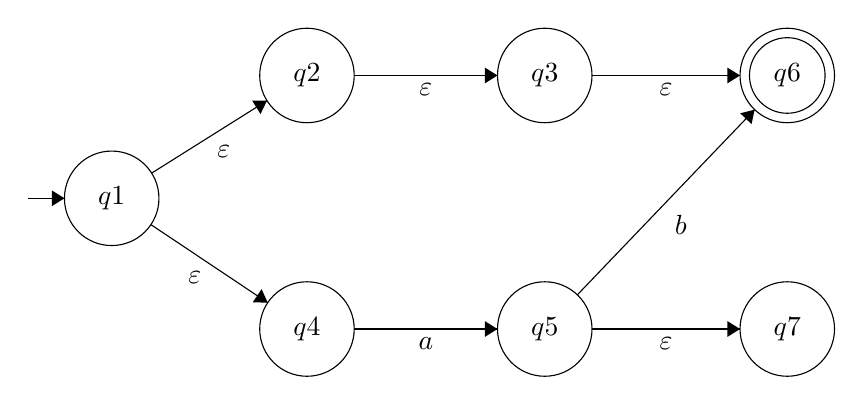
\begin{tikzpicture}[scale=0.2]
\tikzstyle{every node}+=[inner sep=0pt]
\draw [black] (13,-21.7) circle (3);
\draw (13,-21.7) node {$q1$};
\draw [black] (25.4,-13.9) circle (3);
\draw (25.4,-13.9) node {$q2$};
\draw [black] (40.5,-13.9) circle (3);
\draw (40.5,-13.9) node {$q3$};
\draw [black] (55.9,-13.9) circle (3);
\draw (55.9,-13.9) node {$q6$};
\draw [black] (55.9,-13.9) circle (2.4);
\draw [black] (25.4,-30) circle (3);
\draw (25.4,-30) node {$q4$};
\draw [black] (40.5,-30) circle (3);
\draw (40.5,-30) node {$q5$};
\draw [black] (55.9,-30) circle (3);
\draw (55.9,-30) node {$q7$};
\draw [black] (7.7,-21.7) -- (10,-21.7);
\fill [black] (10,-21.7) -- (9.2,-21.2) -- (9.2,-22.2);
\draw [black] (15.54,-20.1) -- (22.86,-15.5);
\fill [black] (22.86,-15.5) -- (21.92,-15.5) -- (22.45,-16.35);
\draw (20.12,-18.3) node [below] {$\varepsilon$};
\draw [black] (15.49,-23.37) -- (22.91,-28.33);
\fill [black] (22.91,-28.33) -- (22.52,-27.47) -- (21.96,-28.3);
\draw (18.28,-26.35) node [below] {$\varepsilon$};
\draw [black] (28.4,-13.9) -- (37.5,-13.9);
\fill [black] (37.5,-13.9) -- (36.7,-13.4) -- (36.7,-14.4);
\draw (32.95,-14.4) node [below] {$\varepsilon$};
\draw [black] (43.5,-13.9) -- (52.9,-13.9);
\fill [black] (52.9,-13.9) -- (52.1,-13.4) -- (52.1,-14.4);
\draw (48.2,-14.4) node [below] {$\varepsilon$};
\draw [black] (43.5,-30) -- (52.9,-30);
\fill [black] (52.9,-30) -- (52.1,-29.5) -- (52.1,-30.5);
\draw (48.2,-30.5) node [below] {$\varepsilon$};
\draw [black] (42.57,-27.83) -- (53.83,-16.07);
\fill [black] (53.83,-16.07) -- (52.91,-16.3) -- (53.63,-16.99);
\draw (48.73,-23.42) node [right] {$b$};
\draw [black] (28.4,-30) -- (37.5,-30);
\fill [black] (37.5,-30) -- (36.7,-29.5) -- (36.7,-30.5);
\draw (32.95,-30.5) node [below] {$a$};
\end{tikzpicture}
\end{center}

Bestimme E-Hülle(q1):
\begin{enumerate}
\item $q_1 \in \varepsilon-Hulle(q_1)$
\item Finde alle Zustände aus $\delta(q_1, \varepsilon) = \{q_2, q_4\} \Rightarrow \{q_2, q_4\} \subseteq \varepsilon-Hulle$
\end{enumerate}

\end{beispiel}

\begin{definition}[$\varepsilon$-Hülle einer Menge $S$ von Zuständen]
\[
\varepsilon\textrm{-Hülle}(S) = \bigcup\limits_{q\in S} \varepsilon\textrm{-Hülle}(q)
\]
\end{definition}

\section{Erweiterung der Übergangsfunktion auf Wörter}

Finde alle Pfade im Graphen, die mit dem Wort $w$ beschriftet sind (mit beliebig vielen $\varepsilon$ dazwischen).

\begin{definition}[Rekursive Definition]
Nun denn:
\begin{itemize}
\item $\hat\delta(q, \varepsilon) = \varepsilon$-Hülle$(q)$
\item $\hat\delta(q, xa)$ wird für $x \in \Sigma^*$  und $a \in \Sigma$ definiert durch:
\begin{enumerate}
\item Sei $\hat\delta(a,x) = \{ p_1, \dots, p_k \}$
\item Sei $\bigcup\limits_{i=1}^k \delta(p_i, a) = \{r_1, \dots, r_m \}$
\item Dann gilt $\hat\delta(q, xa) = \varepsilon$-Hülle$(\{r_1, \dots, r_m\}) = \bigcup\limits_{i=1}^m \varepsilon$-Hülle$(r_i)$
\end{enumerate}
\end{itemize}
\end{definition}

\begin{beispiel}[$\hat\delta(q_0, \textrm{5,6})$] hmm...
\begin{enumerate}
\item $\hat\delta(q_0, \varepsilon) = \varepsilon$-Hülle$(q_0) = \{q_0, q_1 \}$
\item $\hat\delta(q_0, 5)$: $\delta(q_0, 5) \cup \delta(q_1, 5) = \varnothing \cup \{q_1, q_4\}$

$\hat\delta(q_0, 5) = \varepsilon$-Hülle$(q_1) \cup \varepsilon$-Hülle$(q_4) = \{q_1, q_4\}$

\item $\hat\delta(q_0, \textrm{5.})$: $\delta(q_1, \textrm{.}) \cup \delta(q_4, \textrm{.}) = \{q_2\} \cup \{q_3\}  = \{q_2, q_3\}$

$\hat\delta(q_0, \textrm{5.}) = \varepsilon$-Hülle$(q_2) \cup \varepsilon$-Hülle$(q_3) = \{q_2, q_3, q_5\}$

\item $\hat\delta(q_0, \textrm{5.6})$: $\delta(q_2, \textrm{6}) \cup \delta(q_3, \textrm{6}) \cup \delta(q_5, 6) = \{q_2\} \cup \{q_3\}  = \{q_2, q_3\}$

$\hat\delta(q_0, \textrm{5.}) = \varepsilon$-Hülle$(q_2) \cup \varepsilon$-Hülle$(q_3) = \{q_2, q_3, q_5\}$
...
\end{enumerate}
\end{beispiel}

\begin{definition}
Für einen $\varepsilon$-NEA $E = (Q, \Sigma, \delta, q_0, F)$ ist $L(E) = \{w | \hat\delta(q_0, w) \cap F \neq \varnothing\}$.
\end{definition}

\section{Umwandlung von $\varepsilon$-NEAs in DEAs}

Schritt 1: $\varepsilon$-Übergänge eliminieren

Sei $E = (Q_E, \Sigma, \delta_E, q_0, F_E)$ ein $\varepsilon$-NEA. Konstruiere einen äquivalenten DEA $D = (Q_D, \Sigma,
\delta_D, q_{0,D}, F_D)$.
\begin{itemize}
\item $Q_0 = 2^{Q_E}$. Alle erreichbaren Zustände sind $\varepsilon$-abgeschlossene Teilmengen, das heisst Mengen
$S \subseteq Q_E$, so dass $S = \varepsilon$-Hülle$(S)$. D.h. jeder $\varepsilon$-Übergang von einem Zustand $q \in S$ führt
zu einem Zustand, der auch in $S$ liegt.
\item $q_{0,D} = \varepsilon$-Hülle$(q_0)$
\item $F_D = \{ S \in Q_D | S \cap F_E \neq \varnothing \}$
\item $\delta_D(S, a)$ wird für alle $S \in Q_D$ und $a \in \Sigma$ wie folgt berechnet:
\begin{enumerate}
\item Sei $S = \{ p_1, \dots, p_k\}$
\item Berechne $\bigcup\limits_{i=1}^k \delta(p_i, a) = \{r_1, \dots, r_m \}$
\item Dann ist $\delta_D(S, a) = \bigcup\limits_{j=1}^n \varepsilon$-Hüllen$(r_j)$
\end{enumerate}
\end{itemize}

\begin{beispiel}[Von vorher]
Äquivalenter DEA $D$: Startzustand ist $\varepsilon$-Hülle$(q_0) = \{q_0, q_1\}$

Finde die Folgezustände von $\{q_0, q_1\}$ für alle Symbole des Alphabets:
\begin{description}
\item[$+, -$] Kein Übergang von $q_1$ aus, aber von $q_0$ nach $q_1$. Daraus folgt $\varepsilon$-Hülle$(q_1) = \{q_1\}$.
\item[$.$] Kein Übergang von $q_0$, aber von $q_0$ nach $q_2$. Daraus folgt $\varepsilon$-Hülle$(q_2) = \{q_2\}$.
\item[$0,1,\dots,9$] Kein Übergang von $q_0$, aber von $q_1$ nach $q_1$ oder $q_4$. Daraus folgt $\varepsilon$-Hülle$(q_1,q_4)
= \{q_1, q_4\}$
\end{description}

Transitionstabelle (siehe Excel => transferieren)!

\begin{center}
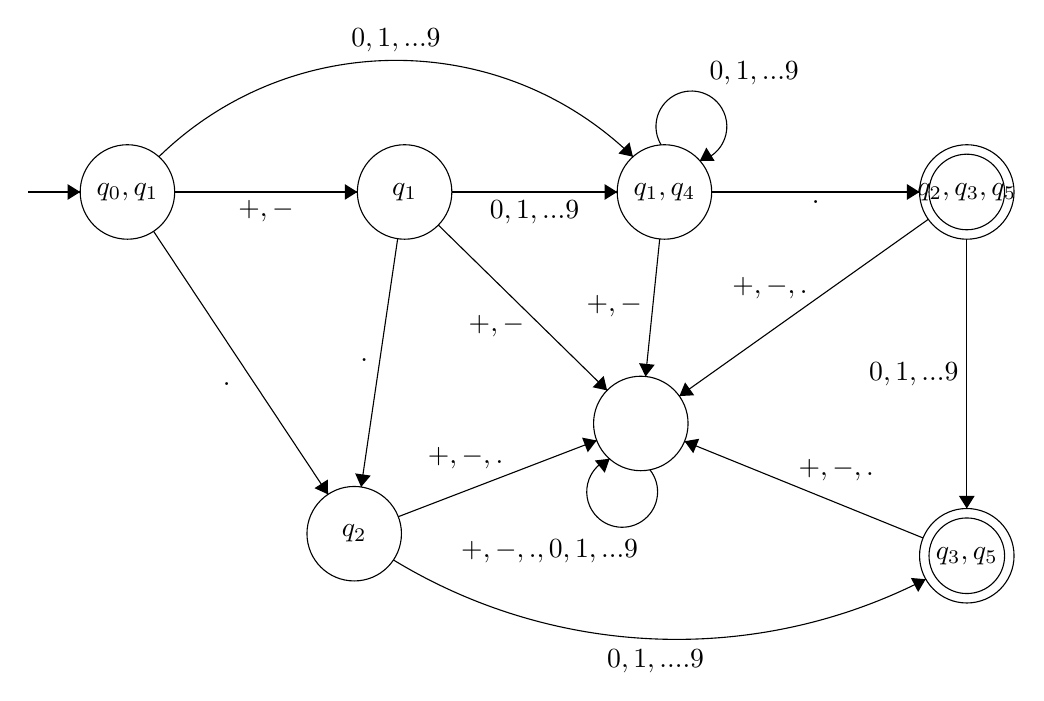
\begin{tikzpicture}[scale=0.2]
\tikzstyle{every node}+=[inner sep=0pt]
\draw [black] (7.9,-20.2) circle (3);
\draw (7.9,-20.2) node {$q_0,q_1$};
\draw [black] (25.5,-20.2) circle (3);
\draw (25.5,-20.2) node {$q_1$};
\draw [black] (42,-20.2) circle (3);
\draw (42,-20.2) node {$q_1,q_4$};
\draw [black] (61.2,-20.2) circle (3);
\draw (61.2,-20.2) node {$q_2,q_3,q_5$};
\draw [black] (61.2,-20.2) circle (2.4);
\draw [black] (40.5,-34.9) circle (3);
\draw (40.5,-34.9) node {${}$};
\draw [black] (61.2,-43.3) circle (3);
\draw (61.2,-43.3) node {$q_3,q_5$};
\draw [black] (61.2,-43.3) circle (2.4);
\draw [black] (22.3,-41.9) circle (3);
\draw (22.3,-41.9) node {$q_2$};
\draw [black] (10.9,-20.2) -- (22.5,-20.2);
\fill [black] (22.5,-20.2) -- (21.7,-19.7) -- (21.7,-20.7);
\draw (16.7,-20.7) node [below] {$+,-$};
\draw [black] (9.896,-17.964) arc (134.26232:45.73768:21.569);
\fill [black] (40,-17.96) -- (39.78,-17.05) -- (39.08,-17.76);
\draw (24.95,-11.34) node [above] {$0,1,...9$};
\draw [black] (28.5,-20.2) -- (39,-20.2);
\fill [black] (39,-20.2) -- (38.2,-19.7) -- (38.2,-20.7);
\draw (33.75,-20.7) node [below] {$0,1,...9$};
\draw [black] (45,-20.2) -- (58.2,-20.2);
\fill [black] (58.2,-20.2) -- (57.4,-19.7) -- (57.4,-20.7);
\draw (51.6,-20.7) node [below] {$.$};
\draw [black] (41.797,-17.219) arc (211.61986:-76.38014:2.25);
\draw (47.7,-13.41) node [above] {$0,1,...9$};
\fill [black] (44.24,-18.23) -- (45.19,-18.23) -- (44.66,-17.38);
\draw [black] (58.75,-21.94) -- (42.95,-33.16);
\fill [black] (42.95,-33.16) -- (43.89,-33.11) -- (43.31,-32.29);
\draw (48.7,-27.05) node [above] {$+,-,.$};
\draw [black] (61.2,-23.2) -- (61.2,-40.3);
\fill [black] (61.2,-40.3) -- (61.7,-39.5) -- (60.7,-39.5);
\draw (60.7,-31.75) node [left] {$0,1,...9$};
\draw [black] (58.42,-42.17) -- (43.28,-36.03);
\fill [black] (43.28,-36.03) -- (43.83,-36.79) -- (44.21,-35.87);
\draw (52.91,-38.56) node [above] {$+,-,.$};
\draw [black] (41.07,-37.833) arc (38.73124:-249.26876:2.25);
\draw (34.71,-42.22) node [below] {$+,-,.,0,1,...9$};
\fill [black] (38.52,-37.14) -- (37.58,-37.25) -- (38.21,-38.03);
\draw [black] (58.595,-44.785) arc (-62.79869:-121.32365:34.599);
\fill [black] (58.59,-44.79) -- (57.65,-44.71) -- (58.11,-45.6);
\draw (41.44,-49.21) node [below] {$0,1,....9$};
\draw [black] (25.1,-40.82) -- (37.7,-35.98);
\fill [black] (37.7,-35.98) -- (36.77,-35.8) -- (37.13,-36.73);
\draw (29.37,-37.85) node [above] {$+,-,.$};
\draw [black] (25.06,-23.17) -- (22.74,-38.93);
\fill [black] (22.74,-38.93) -- (23.35,-38.21) -- (22.36,-38.07);
\draw (23.21,-30.87) node [left] {$.$};
\draw [black] (9.56,-22.7) -- (20.64,-39.4);
\fill [black] (20.64,-39.4) -- (20.62,-38.46) -- (19.78,-39.01);
\draw (14.49,-32.38) node [left] {$.$};
\draw [black] (1.6,-20.2) -- (4.9,-20.2);
\fill [black] (4.9,-20.2) -- (4.1,-19.7) -- (4.1,-20.7);
\draw [black] (41.7,-23.18) -- (40.8,-31.92);
\fill [black] (40.8,-31.92) -- (41.38,-31.17) -- (40.39,-31.07);
\draw (40.61,-27.46) node [left] {$+,-$};
\draw [black] (27.64,-22.3) -- (38.36,-32.8);
\fill [black] (38.36,-32.8) -- (38.14,-31.88) -- (37.44,-32.6);
\draw (31.33,-28.03) node [below] {$+,-$};
\end{tikzpicture}
\end{center}


\end{beispiel}

\begin{bemerkung}[Konvention]
Die da wären:
\begin{itemize}
\item Der Zustand $\varnothing$ wird Senkezustand (Abfallzustand) genannt und darf weggelassen werden.
\item Darstellung eines DEA mit fehlenden Transitionen sind immer so zu verstehen, dass die fehlenden Transitionen in einen solchen Senkezustand führen:
\begin{center}
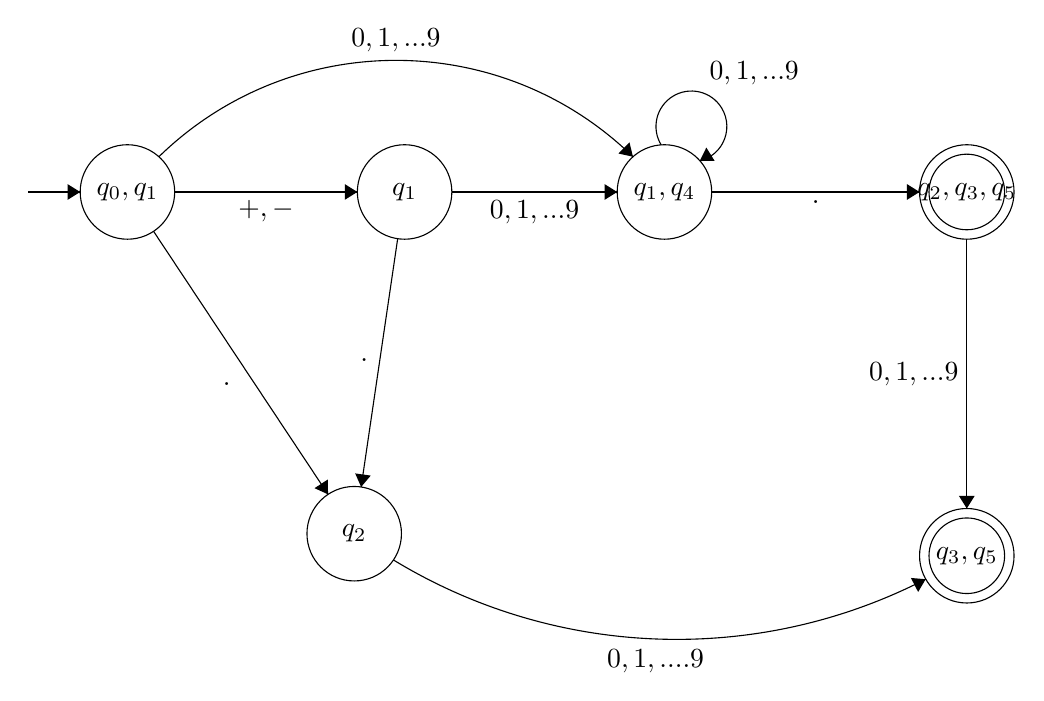
\begin{tikzpicture}[scale=0.2]
\tikzstyle{every node}+=[inner sep=0pt]
\draw [black] (7.9,-20.2) circle (3);
\draw (7.9,-20.2) node {$q_0,q_1$};
\draw [black] (25.5,-20.2) circle (3);
\draw (25.5,-20.2) node {$q_1$};
\draw [black] (42,-20.2) circle (3);
\draw (42,-20.2) node {$q_1,q_4$};
\draw [black] (61.2,-20.2) circle (3);
\draw (61.2,-20.2) node {$q_2,q_3,q_5$};
\draw [black] (61.2,-20.2) circle (2.4);
\draw [black] (61.2,-43.3) circle (3);
\draw (61.2,-43.3) node {$q_3,q_5$};
\draw [black] (61.2,-43.3) circle (2.4);
\draw [black] (22.3,-41.9) circle (3);
\draw (22.3,-41.9) node {$q_2$};
\draw [black] (10.9,-20.2) -- (22.5,-20.2);
\fill [black] (22.5,-20.2) -- (21.7,-19.7) -- (21.7,-20.7);
\draw (16.7,-20.7) node [below] {$+,-$};
\draw [black] (9.896,-17.964) arc (134.26232:45.73768:21.569);
\fill [black] (40,-17.96) -- (39.78,-17.05) -- (39.08,-17.76);
\draw (24.95,-11.34) node [above] {$0,1,...9$};
\draw [black] (28.5,-20.2) -- (39,-20.2);
\fill [black] (39,-20.2) -- (38.2,-19.7) -- (38.2,-20.7);
\draw (33.75,-20.7) node [below] {$0,1,...9$};
\draw [black] (45,-20.2) -- (58.2,-20.2);
\fill [black] (58.2,-20.2) -- (57.4,-19.7) -- (57.4,-20.7);
\draw (51.6,-20.7) node [below] {$.$};
\draw [black] (41.797,-17.219) arc (211.61986:-76.38014:2.25);
\draw (47.7,-13.41) node [above] {$0,1,...9$};
\fill [black] (44.24,-18.23) -- (45.19,-18.23) -- (44.66,-17.38);
\draw [black] (61.2,-23.2) -- (61.2,-40.3);
\fill [black] (61.2,-40.3) -- (61.7,-39.5) -- (60.7,-39.5);
\draw (60.7,-31.75) node [left] {$0,1,...9$};
\draw [black] (58.595,-44.785) arc (-62.79869:-121.32365:34.599);
\fill [black] (58.59,-44.79) -- (57.65,-44.71) -- (58.11,-45.6);
\draw (41.44,-49.21) node [below] {$0,1,....9$};
\draw [black] (25.06,-23.17) -- (22.74,-38.93);
\fill [black] (22.74,-38.93) -- (23.35,-38.21) -- (22.36,-38.07);
\draw (23.21,-30.87) node [left] {$.$};
\draw [black] (9.56,-22.7) -- (20.64,-39.4);
\fill [black] (20.64,-39.4) -- (20.62,-38.46) -- (19.78,-39.01);
\draw (14.49,-32.38) node [left] {$.$};
\draw [black] (1.6,-20.2) -- (4.9,-20.2);
\fill [black] (4.9,-20.2) -- (4.1,-19.7) -- (4.1,-20.7);
\end{tikzpicture}
\end{center}
\end{itemize}
\end{bemerkung}

Zusammenfassung: DEAs und $\varepsilon$-NEAs sind äquivalent.

\begin{center}
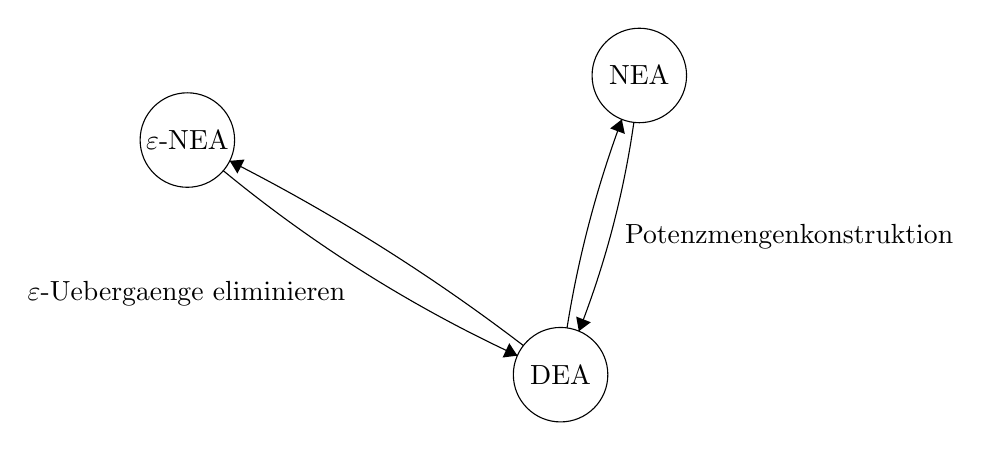
\begin{tikzpicture}[scale=0.2]
\tikzstyle{every node}+=[inner sep=0pt]
\draw [black] (12.3,-23.3) circle (3);
\draw (12.3,-23.3) node {$\varepsilon$-NEA};
\draw [black] (41,-19.2) circle (3);
\draw (41,-19.2) node {NEA};
\draw [black] (36,-38.2) circle (3);
\draw (36,-38.2) node {DEA};
\draw [black] (36.409,-35.228) arc (170.92969:159.58319:69.248);
\fill [black] (39.89,-21.99) -- (39.15,-22.56) -- (40.08,-22.91);
\draw [black] (40.653,-22.18) arc (-8.09337:-21.39375:59.182);
\fill [black] (37.16,-35.44) -- (37.92,-34.87) -- (36.99,-34.51);
\draw (40.06,-29.41) node [right] {Potenzmengenkonstruktion};
\draw [black] (33.256,-36.988) arc (-114.82059:-129.4939:86.368);
\fill [black] (33.26,-36.99) -- (32.74,-36.2) -- (32.32,-37.11);
\draw (12.24,-32.22) node [below] {$\varepsilon$-Uebergaenge eliminieren};
\draw [black] (14.992,-24.625) arc (63.08039:52.60511:120.648);
\fill [black] (14.99,-24.62) -- (15.48,-25.43) -- (15.93,-24.54);
\end{tikzpicture}
\end{center}

\section{Reguläre Ausdrücke}

Besonders geeignet für die Mustersuche, anderer Formalismus zur Beschreibung von regulären Sprachen.

\section{Operatoren für reguläre Ausdrücken}

\begin{itemize}
\item Die Vereinigung von Sprachen $L$ und $M$, $L \cup M$, ist die Menge aller Zeichenreihen, die entweder in $L$ oder in $M$ oder in beiden enthalten sind.
\item Die Verkettung (Konkatenation) von $L$ und $M$, $L\cdot M$ oder $LM$, ist die Menge aller Zeichenreihe, gebildet aus einer Verkettung einer Zeichenreihe aus $L$ umit einer beliebigen aus $M$.

Formal: \[
LM = \{w \in \Sigma^* | w = uv \textrm{ mit } u \in L \textrm{ und } v \in M \}
\]

\item Die Kleensche Hülle (Stern) von $L$, $L^*$, ist die Menge aller Zeichenreihen, die durch die Verkettung einer beliebigen Anzahl von Zeichenreihen aus $L$ gebildet wird.

Formal:
\begin{eqnarray*}
L^0 &=& \{\varepsilon\} \\
L^1 &=& L \\
L^n &=& L\cdot L^{n-1} \\
L^* &=& \bigcup\limits_{i=0}^\infty L^i
\end{eqnarray*}

Anschaulich: $w \in L^*$, wenn sich $w$ zerlegen lässt in endlich viele Wörter $w = w_1w_2\dots w_k$ für ein $k \in \mathbb{N}$, so dass $w_1\in L_1, w_2 \in L_2 \dots w_i L_i$ gilt.

Spezialfälle:
\begin{itemize}
\item $\varnothing^* = \{\varepsilon\}$, da $\varnothing^0 = \{\varepsilon\}$
\item $\{\varepsilon\}^* = \{\varepsilon\}$
\end{itemize}
Aber: $\varnothing^i = \varnothing$ für $i > 1$.

\end{itemize}

\begin{definition}[Reguläre Ausdrücke]
Reguläre Ausdrücke lassen sich wie folgt definieren:
\begin{enumerate}
\item $\varepsilon$ und $\varnothing$ sind reguläre Ausdrücke.
\item Jedes Symbol $a \in \Sigma$ ist ein regulärer Ausdruck.
\item Wenn $\alpha$ und $\beta$ reguläre Ausdrücke sind, dann sind:
\begin{itemize}
\item $(\alpha\cdot\beta)$ (Konkatenation)
\item $(\alpha+\beta)$ (Vereinigung)
\end{itemize}
reguläre Ausdrücke.
\item Wenn $\alpha$ ein regulärer Ausdruck ist, dan ist auch $(\alpha)^*$ ein regulärer Ausdruck. (Kleenscher Stern)
\end{enumerate}

\end{definition}

\begin{bemerkung}[Konvention] Man tut:
\begin{itemize}
\item Überflüssige Klammern weglassen
\item Stern bindet stärker als Verkettung
\item Verkettung bindet stärker als Vereinigung
\end{itemize}
\end{bemerkung}

\section{Bedeutung regulärer Ausdrücke}

$L(\alpha)$ bezeichnet die durch den regulären Ausdruck beschriebene Sprache. Dabei gilt: \begin{itemize}
\item $L(\varepsilon) = \{\varepsilon\}$
\item $L(\varnothing) = \varnothing$
\item $L(a) = \{a \}$
\item $L(\alpha\cdot\beta) = L(\alpha)\cdot L(\beta)$
\item $L(\alpha + \beta) = L(\alpha) \cup L(\beta)$
\item $L(\alpha^*) = (L(\alpha))^*$
\end{itemize}

\begin{beispiel}[Beschreibung von Sprachen durch reguläre Ausdrücke]
Nun:
\begin{enumerate}
\item $L_1 = \{ w \in \{0,1\}^* | w$ beginnt mit 011 und enthält das Teilwort 00 $\}$.
RA für $L_1$: $011\cdot(0+1)^*\cdot 00 \cdot (0+1)^*$

\item $L_2 = \{ w \in \{a,b,c\}^* | |w|_a$ ist gerade $\}$.

RA für $L_2$: $\left( (b+c)^* a (b+c)^* a (b+c)^* \right)^*$

\item $L_3 = \{ w \in \{0,1\}^* | $ In $w$ kommen die Nullen und Einsen immer abwechselnd vor$\}$

RA für $L_3$: $(01)^* + (10)^* + 1(01)^* + 0(10)^* = (\varepsilon + 1)(01)^*(\varepsilon + 0)$
\end{enumerate}

\end{beispiel}

\begin{center}
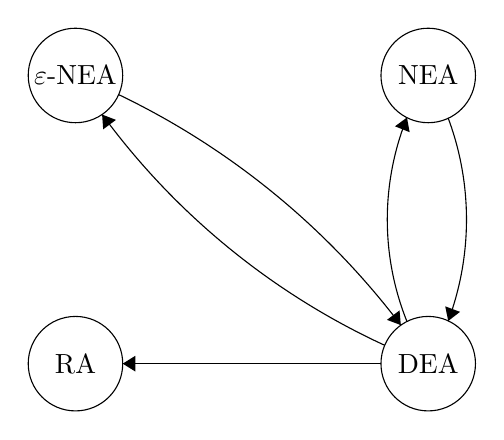
\begin{tikzpicture}[scale=0.2]
\tikzstyle{every node}+=[inner sep=0pt]
\draw [black] (11.2,-21.9) circle (3);
\draw (11.2,-21.9) node {$\varepsilon$-NEA};
\draw [black] (33.6,-21.9) circle (3);
\draw (33.6,-21.9) node {NEA};
\draw [black] (11.2,-40.2) circle (3);
\draw (11.2,-40.2) node {RA};
\draw [black] (33.6,-40.2) circle (3);
\draw (33.6,-40.2) node {DEA};
\draw [black] (30.6,-40.2) -- (14.2,-40.2);
\fill [black] (14.2,-40.2) -- (15,-40.7) -- (15,-39.7);
\draw [black] (34.87,-24.614) arc (20.42466:-20.42466:18.442);
\fill [black] (34.87,-37.49) -- (35.62,-36.91) -- (34.68,-36.56);
\draw [black] (32.25,-37.525) arc (-158.15239:-201.84761:17.4);
\fill [black] (32.25,-24.57) -- (31.49,-25.13) -- (32.42,-25.5);
\draw [black] (13.942,-23.115) arc (64.3583:37.14651:49.183);
\fill [black] (31.86,-37.75) -- (31.78,-36.82) -- (30.98,-37.42);
\draw [black] (30.837,-39.034) arc (-114.74075:-143.75444:46.246);
\fill [black] (12.89,-24.38) -- (12.96,-25.32) -- (13.77,-24.72);
\end{tikzpicture}
\end{center}

Lösung der Aufgabe 6 (Aufgabenblatt 2):

\begin{itemize}[a)]
\item $(a+b)^*: \{a,b\}^*$.

$(a^*b^*): \varepsilon \in \mathcal{L}(a^*)$ und $\varepsilon \in \mathcal{L}(b^*)$.
$\Rightarrow a \in \mathcal{L}(a^*b^*)$ und $b \in \mathcal{L}(a^*b^*)$
\end{itemize}

\section{Anwendungsbeispiel für RA}

Spezifikation einer Eingabemaske für Kontostände. Bedingungen:
\begin{itemize}
\item Währungseingabe: CHF, EUR, USD
\item optionales Vorzeichen vor dem Betrag: $\oplus$, $\ominus$
\item Betrag ganzzahlig oder mit Dezimalpunkt und zwei Nachkommastellen
\item keine führende Nullen
\end{itemize}

$\Sigma = \{C,D,E,F,H,R,S,U,\oplus, \ominus, ., 0, 1, \dots, 9\}$

Idee: Setze den RA aus Teilen zusammen:

zahlung = waehrung vorzeichen betrag

waehrung = $(CHF + EUR + USD)$

vorzeichen = $(\varepsilon + \oplus + \ominus)$

betrag = ganzzahl ($\varepsilon + .$nachkomma$)$

ganzzahl  = $(0 + (1+2+\dots+9)(0 + 1 +\dots+9)^*$

nachkomma = $(0,1,\dots,9)+(0,1,\dots,9)$

\newcommand{\enea}{$\varepsilon$-NEA}

$\Rightarrow $ zahlung =  $(CHF + EUR + USD)$ $(\varepsilon + \oplus + \ominus)$ $(0 + (1+2+\dots+9)(0 + 1 +\dots+9)^*$
($\varepsilon + .$(0,1,\dots,9)+(0,1,\dots,9)$)$

\section{Eine ganz neue Idee}

\begin{theorem}
Reguläre Ausdrücke und endliche Automaten sind äquivalent:
\begin{enumerate}
\item für jeden RA $\alpha$ existiert ein DEA $A_\alpha$ mit $\mathcal{L}(\alpha) = \mathcal{L}(A_\alpha)$
\item für jeden DEA $A$ existiert ein RA $\alpha_A$ mit $\mathcal{L}(A) = \mathcal{L}(\alpha_A)$
\end{enumerate}
\end{theorem}

\begin{proof}[Beweis für 1.] Nun.
Umwandlung von RA in DEA. Vorgehensweise: RA $\mapsto$ \enea $\mapsto$ DEA. Für einen gegebenen RA konstruiere einen $\varepsilon$-NEA induktiv entsprechend des regulären Ausdrucks des RA mit folgenden zusätzlichen Eigenschaften:
\begin{enumerate}
\item genau ein akzeptierender Zustand
\item keine Transitionen zum Startzustand
\item keine Transitionen vom akzeptierenden Zustand wegführende Transitionen
\end{enumerate}
Induktionsanfang: \enea für $\varepsilon$:

\begin{center}
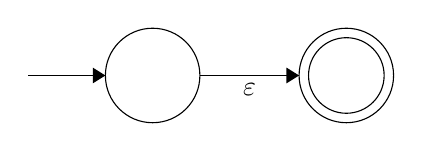
\begin{tikzpicture}[scale=0.2]
\tikzstyle{every node}+=[inner sep=0pt]
\draw [black] (17.9,-16.2) circle (3);
\draw [black] (30.2,-16.2) circle (3);
\draw [black] (30.2,-16.2) circle (2.4);
\draw [black] (10,-16.2) -- (14.9,-16.2);
\fill [black] (14.9,-16.2) -- (14.1,-15.7) -- (14.1,-16.7);
\draw [black] (20.9,-16.2) -- (27.2,-16.2);
\fill [black] (27.2,-16.2) -- (26.4,-15.7) -- (26.4,-16.7);
\draw (24.05,-16.7) node [below] {$\varepsilon$};
\end{tikzpicture}
\end{center}

\enea für $\varnothing$:

\begin{center}
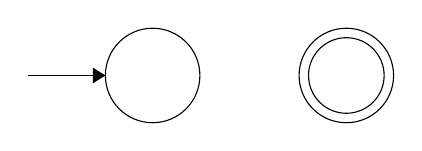
\begin{tikzpicture}[scale=0.2]
\tikzstyle{every node}+=[inner sep=0pt]
\draw [black] (17.9,-16.2) circle (3);
\draw [black] (30.2,-16.2) circle (3);
\draw [black] (30.2,-16.2) circle (2.4);
\draw [black] (10,-16.2) -- (14.9,-16.2);
\fill [black] (14.9,-16.2) -- (14.1,-15.7) -- (14.1,-16.7);
\end{tikzpicture}
\end{center}

\enea für $a \in \Sigma$:

\begin{center}
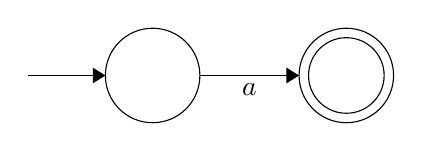
\begin{tikzpicture}[scale=0.2]
\tikzstyle{every node}+=[inner sep=0pt]
\draw [black] (17.9,-16.2) circle (3);
\draw [black] (30.2,-16.2) circle (3);
\draw [black] (30.2,-16.2) circle (2.4);
\draw [black] (10,-16.2) -- (14.9,-16.2);
\fill [black] (14.9,-16.2) -- (14.1,-15.7) -- (14.1,-16.7);
\draw [black] (20.9,-16.2) -- (27.2,-16.2);
\fill [black] (27.2,-16.2) -- (26.4,-15.7) -- (26.4,-16.7);
\draw (24.05,-16.7) node [below] {$a$};
\end{tikzpicture}
\end{center}

Induktionsschritt:
\begin{itemize}
\item Sei $\alpha = \beta + \gamma$ ein RA, seien $B$ und $C$ \enea s für $\beta$ und $\gamma$ wie oben und mit Startzuständen $q_{B0}$ und $q_{C0}$ und akzeptierenden Zuständen $q_{BF}$ und $q_{CF}$.

Konstruiere hieraus einen \enea für $\alpha$ wie folgt:

\begin{center}
\begin{tikzpicture}[scale=0.2]
\tikzstyle{every node}+=[inner sep=0pt]
\draw [black] (21.8,-17.3) circle (3);
\draw (21.8,-17.3) node {$qB0$};
\draw [black] (53.8,-17.3) circle (3);
\draw (53.8,-17.3) node {$qBF$};
%\draw [black] (38.1,-17.3) circle (3);
\draw (38.1,-17.3) node {$B$};
\draw [black] (21.8,-34.6) circle (3);
\draw (21.8,-34.6) node {$qC0$};
%\draw [black] (38.1,-34.6) circle (3);
\draw (38.1,-34.6) node {$C$};
\draw [black] (53.8,-34.6) circle (3);
\draw (53.8,-34.6) node {$qCF$};
\draw [black] (8.9,-26) circle (3);
\draw [black] (67.6,-26) circle (3);
\draw [black] (67.6,-26) circle (2.4);
\draw [black] (2.1,-26) -- (5.9,-26);
\fill [black] (5.9,-26) -- (5.1,-25.5) -- (5.1,-26.5);
\draw [black] (11.39,-24.32) -- (19.31,-18.98);
\fill [black] (19.31,-18.98) -- (18.37,-19.01) -- (18.93,-19.84);
\draw (16.27,-22.15) node [below] {$\varepsilon$};
\draw [black] (11.4,-27.66) -- (19.3,-32.94);
\fill [black] (19.3,-32.94) -- (18.92,-32.08) -- (18.36,-32.91);
\draw (14.43,-30.8) node [below] {$\varepsilon$};
\draw [black] (56.34,-18.9) -- (65.06,-24.4);
\fill [black] (65.06,-24.4) -- (64.65,-23.55) -- (64.12,-24.4);
\draw (59.78,-22.15) node [below] {$\varepsilon$};
\draw [black] (56.35,-33.01) -- (65.05,-27.59);
\fill [black] (65.05,-27.59) -- (64.11,-27.59) -- (64.64,-28.43);
\draw (61.62,-30.8) node [below] {$\varepsilon$};
\end{tikzpicture}
\end{center}

erfüllt alle Bedingungen.

\item Seien $\alpha = \beta\cdot\gamma$ und $B,C$ \enea s für $\beta$, $\gamma$. \enea für $\alpha$:

\begin{center}
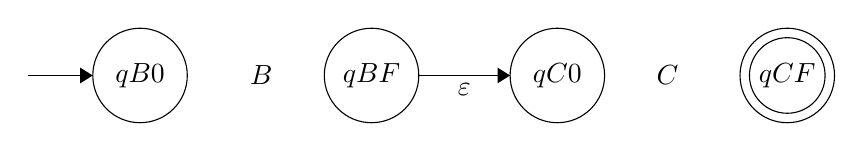
\begin{tikzpicture}[scale=0.2]
\tikzstyle{every node}+=[inner sep=0pt]
\draw [black] (21.8,-17.3) circle (3);
\draw (21.8,-17.3) node {$qB0$};
\draw [black] (36.5,-17.3) circle (3);
\draw (36.5,-17.3) node {$qBF$};
%\draw [black] (29.5,-17.3) circle (3);
\draw (29.5,-17.3) node {$B$};
\draw [black] (48.3,-17.3) circle (3);
\draw (48.3,-17.3) node {$qC0$};
%\draw [black] (55.3,-17.3) circle (3);
\draw (55.3,-17.3) node {$C$};
\draw [black] (62.9,-17.3) circle (3);
\draw (62.9,-17.3) node {$qCF$};
\draw [black] (62.9,-17.3) circle (2.4);
\draw [black] (14.7,-17.3) -- (18.8,-17.3);
\fill [black] (18.8,-17.3) -- (18,-16.8) -- (18,-17.8);
\draw [black] (39.5,-17.3) -- (45.3,-17.3);
\fill [black] (45.3,-17.3) -- (44.5,-16.8) -- (44.5,-17.8);
\draw (42.4,-17.8) node [below] {$\varepsilon$};
\end{tikzpicture}
\end{center}

erfüllt alle Bedingungen.

\item Sei $\alpha = \beta^*$, $B$ ein \enea für $\beta$. \enea für $\alpha$:

\begin{center}
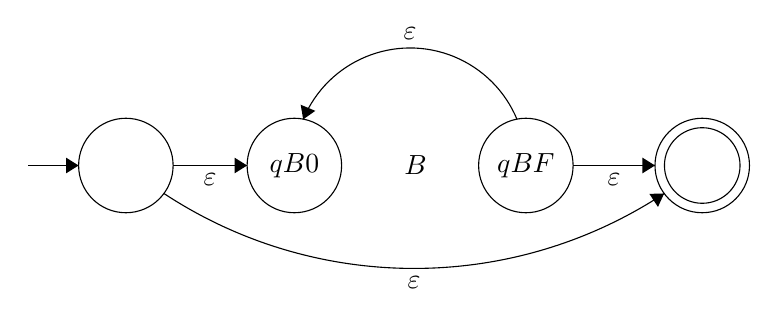
\begin{tikzpicture}[scale=0.2]
\tikzstyle{every node}+=[inner sep=0pt]
\draw [black] (21.8,-17.3) circle (3);
\draw (21.8,-17.3) node {$qB0$};
\draw [black] (36.5,-17.3) circle (3);
\draw (36.5,-17.3) node {$qBF$};
%\draw [black] (29.5,-17.3) circle (3);
\draw (29.5,-17.3) node {$B$};
\draw [black] (11.1,-17.3) circle (3);
\draw [black] (47.7,-17.3) circle (3);
\draw [black] (47.7,-17.3) circle (2.4);
\draw [black] (22.359,-14.374) arc (-202.51215:-337.48785:7.351);
\fill [black] (22.36,-14.37) -- (23.13,-13.83) -- (22.2,-13.44);
\draw (29.15,-9.34) node [above] {$\varepsilon$};
\draw [black] (14.1,-17.3) -- (18.8,-17.3);
\fill [black] (18.8,-17.3) -- (18,-16.8) -- (18,-17.8);
\draw (16.45,-17.8) node [below] {$\varepsilon$};
\draw [black] (4.9,-17.3) -- (8.1,-17.3);
\fill [black] (8.1,-17.3) -- (7.3,-16.8) -- (7.3,-17.8);
\draw [black] (39.5,-17.3) -- (44.7,-17.3);
\fill [black] (44.7,-17.3) -- (43.9,-16.8) -- (43.9,-17.8);
\draw (42.1,-17.8) node [below] {$\varepsilon$};
\draw [black] (45.285,-19.077) arc (-56.63145:-123.36855:28.88);
\fill [black] (45.28,-19.08) -- (44.34,-19.1) -- (44.89,-19.93);
\draw (29.4,-24.34) node [below] {$\varepsilon$};
\end{tikzpicture}
\end{center}

erfüllt alle Bedingungen.

\end{itemize}

\end{proof}

\begin{beispiel}
Beispiel: \enea $A$ für $\alpha = (0+1)^*1(0+1)$:

\enea für $(0+1)$:

\begin{center}
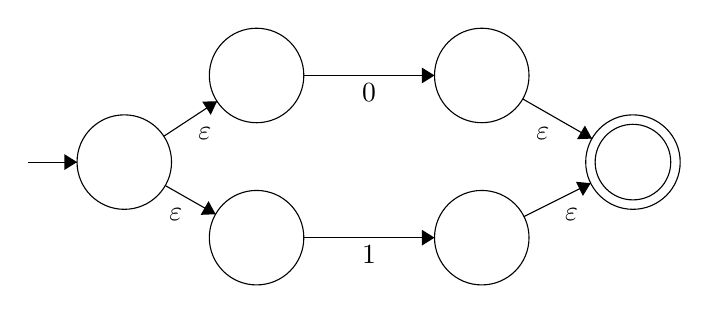
\begin{tikzpicture}[scale=0.2]
\tikzstyle{every node}+=[inner sep=0pt]
\draw [black] (13.2,-22.8) circle (3);
\draw [black] (21.6,-17.3) circle (3);
\draw [black] (21.6,-27.6) circle (3);
\draw [black] (35.9,-17.3) circle (3);
\draw [black] (35.9,-27.6) circle (3);
\draw [black] (45.5,-22.8) circle (3);
\draw [black] (45.5,-22.8) circle (2.4);
\draw [black] (7.1,-22.8) -- (10.2,-22.8);
\fill [black] (10.2,-22.8) -- (9.4,-22.3) -- (9.4,-23.3);
\draw [black] (15.71,-21.16) -- (19.09,-18.94);
\fill [black] (19.09,-18.94) -- (18.15,-18.96) -- (18.69,-19.8);
\draw (18.32,-20.55) node [below] {$\varepsilon$};
\draw [black] (15.8,-24.29) -- (19,-26.11);
\fill [black] (19,-26.11) -- (18.55,-25.28) -- (18.05,-26.15);
\draw (16.48,-25.7) node [below] {$\varepsilon$};
\draw [black] (24.6,-17.3) -- (32.9,-17.3);
\fill [black] (32.9,-17.3) -- (32.1,-16.8) -- (32.1,-17.8);
\draw (28.75,-17.8) node [below] {$0$};
\draw [black] (24.6,-27.6) -- (32.9,-27.6);
\fill [black] (32.9,-27.6) -- (32.1,-27.1) -- (32.1,-28.1);
\draw (28.75,-28.1) node [below] {$1$};
\draw [black] (38.5,-18.79) -- (42.9,-21.31);
\fill [black] (42.9,-21.31) -- (42.45,-20.48) -- (41.95,-21.34);
\draw (39.78,-20.55) node [below] {$\varepsilon$};
\draw [black] (38.58,-26.26) -- (42.82,-24.14);
\fill [black] (42.82,-24.14) -- (41.88,-24.05) -- (42.32,-24.95);
\draw (41.61,-25.7) node [below] {$\varepsilon$};
\end{tikzpicture}
\end{center}

\enea für $(0+1)^*$:

\begin{center}
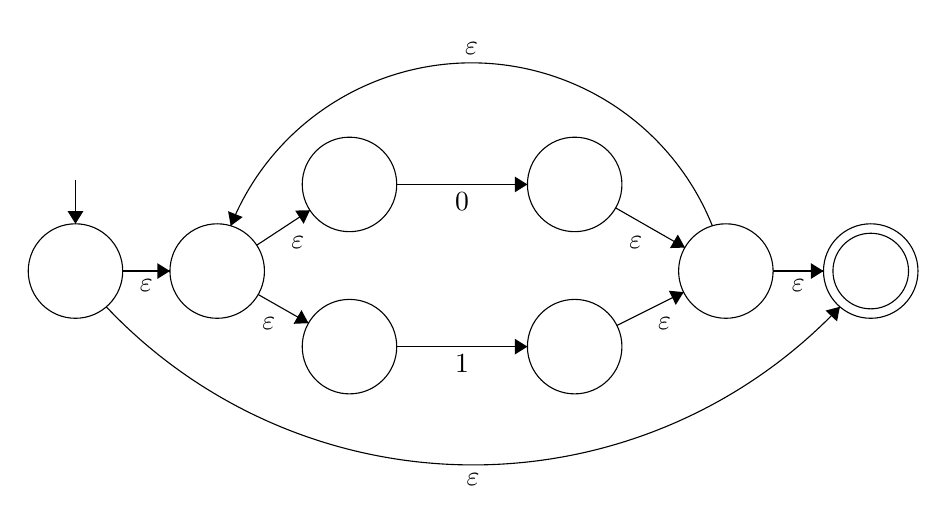
\begin{tikzpicture}[scale=0.2]
\tikzstyle{every node}+=[inner sep=0pt]
\draw [black] (13.2,-22.8) circle (3);
\draw [black] (21.6,-17.3) circle (3);
\draw [black] (21.6,-27.6) circle (3);
\draw [black] (35.9,-17.3) circle (3);
\draw [black] (35.9,-27.6) circle (3);
\draw [black] (45.5,-22.8) circle (3);
\draw [black] (54.7,-22.8) circle (3);
\draw [black] (54.7,-22.8) circle (2.4);
\draw [black] (4.2,-22.8) circle (3);
\draw [black] (15.71,-21.16) -- (19.09,-18.94);
\fill [black] (19.09,-18.94) -- (18.15,-18.96) -- (18.69,-19.8);
\draw (18.32,-20.55) node [below] {$\varepsilon$};
\draw [black] (15.8,-24.29) -- (19,-26.11);
\fill [black] (19,-26.11) -- (18.55,-25.28) -- (18.05,-26.15);
\draw (16.48,-25.7) node [below] {$\varepsilon$};
\draw [black] (24.6,-17.3) -- (32.9,-17.3);
\fill [black] (32.9,-17.3) -- (32.1,-16.8) -- (32.1,-17.8);
\draw (28.75,-17.8) node [below] {$0$};
\draw [black] (24.6,-27.6) -- (32.9,-27.6);
\fill [black] (32.9,-27.6) -- (32.1,-27.1) -- (32.1,-28.1);
\draw (28.75,-28.1) node [below] {$1$};
\draw [black] (38.5,-18.79) -- (42.9,-21.31);
\fill [black] (42.9,-21.31) -- (42.45,-20.48) -- (41.95,-21.34);
\draw (39.78,-20.55) node [below] {$\varepsilon$};
\draw [black] (38.58,-26.26) -- (42.82,-24.14);
\fill [black] (42.82,-24.14) -- (41.88,-24.05) -- (42.32,-24.95);
\draw (41.61,-25.7) node [below] {$\varepsilon$};
\draw [black] (48.5,-22.8) -- (51.7,-22.8);
\fill [black] (51.7,-22.8) -- (50.9,-22.3) -- (50.9,-23.3);
\draw (50.1,-23.3) node [below] {$\varepsilon$};
\draw [black] (7.2,-22.8) -- (10.2,-22.8);
\fill [black] (10.2,-22.8) -- (9.4,-22.3) -- (9.4,-23.3);
\draw (8.7,-23.3) node [below] {$\varepsilon$};
\draw [black] (4.2,-17) -- (4.2,-19.8);
\fill [black] (4.2,-19.8) -- (4.7,-19) -- (3.7,-19);
\draw [black] (14.057,-19.929) arc (158.15526:21.84474:16.476);
\fill [black] (14.06,-19.93) -- (14.82,-19.37) -- (13.89,-19);
\draw (29.35,-9.08) node [above] {$\varepsilon$};
\draw [black] (52.745,-25.074) arc (-43.37782:-136.62218:32.049);
\fill [black] (52.74,-25.07) -- (51.83,-25.31) -- (52.56,-26);
\draw (29.45,-35.61) node [below] {$\varepsilon$};
\end{tikzpicture}
\end{center}

\enea für $(0+1)^*1(0+1)$:

\begin{center}
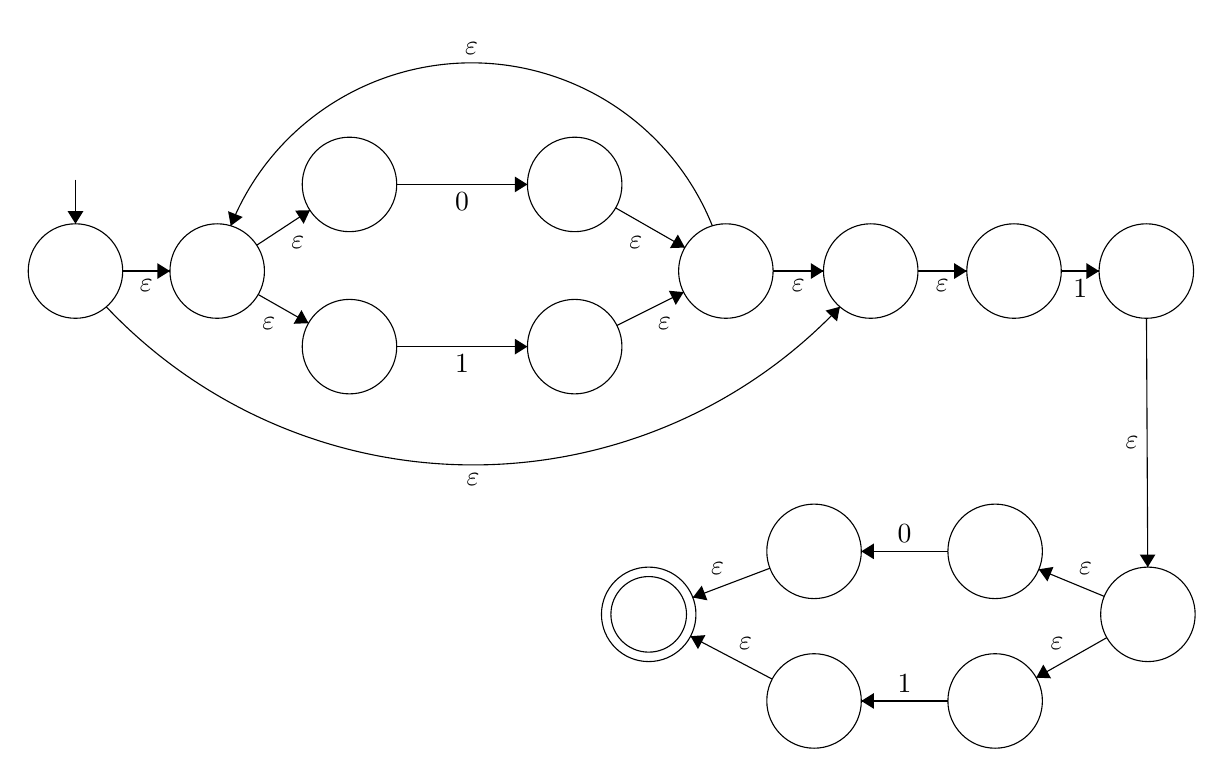
\begin{tikzpicture}[scale=0.2]
\tikzstyle{every node}+=[inner sep=0pt]
\draw [black] (13.2,-22.8) circle (3);
\draw [black] (21.6,-17.3) circle (3);
\draw [black] (21.6,-27.6) circle (3);
\draw [black] (35.9,-17.3) circle (3);
\draw [black] (35.9,-27.6) circle (3);
\draw [black] (45.5,-22.8) circle (3);
\draw [black] (54.7,-22.8) circle (3);
\draw [black] (4.2,-22.8) circle (3);
\draw [black] (63.8,-22.8) circle (3);
\draw [black] (72.2,-22.8) circle (3);
\draw [black] (72.3,-44.6) circle (3);
\draw [black] (62.6,-40.6) circle (3);
\draw [black] (62.6,-50.1) circle (3);
\draw [black] (51.1,-40.6) circle (3);
\draw [black] (51.1,-50.1) circle (3);
\draw [black] (40.6,-44.6) circle (3);
\draw [black] (40.6,-44.6) circle (2.4);
\draw [black] (15.71,-21.16) -- (19.09,-18.94);
\fill [black] (19.09,-18.94) -- (18.15,-18.96) -- (18.69,-19.8);
\draw (18.32,-20.55) node [below] {$\varepsilon$};
\draw [black] (15.8,-24.29) -- (19,-26.11);
\fill [black] (19,-26.11) -- (18.55,-25.28) -- (18.05,-26.15);
\draw (16.48,-25.7) node [below] {$\varepsilon$};
\draw [black] (24.6,-17.3) -- (32.9,-17.3);
\fill [black] (32.9,-17.3) -- (32.1,-16.8) -- (32.1,-17.8);
\draw (28.75,-17.8) node [below] {$0$};
\draw [black] (24.6,-27.6) -- (32.9,-27.6);
\fill [black] (32.9,-27.6) -- (32.1,-27.1) -- (32.1,-28.1);
\draw (28.75,-28.1) node [below] {$1$};
\draw [black] (38.5,-18.79) -- (42.9,-21.31);
\fill [black] (42.9,-21.31) -- (42.45,-20.48) -- (41.95,-21.34);
\draw (39.78,-20.55) node [below] {$\varepsilon$};
\draw [black] (38.58,-26.26) -- (42.82,-24.14);
\fill [black] (42.82,-24.14) -- (41.88,-24.05) -- (42.32,-24.95);
\draw (41.61,-25.7) node [below] {$\varepsilon$};
\draw [black] (48.5,-22.8) -- (51.7,-22.8);
\fill [black] (51.7,-22.8) -- (50.9,-22.3) -- (50.9,-23.3);
\draw (50.1,-23.3) node [below] {$\varepsilon$};
\draw [black] (7.2,-22.8) -- (10.2,-22.8);
\fill [black] (10.2,-22.8) -- (9.4,-22.3) -- (9.4,-23.3);
\draw (8.7,-23.3) node [below] {$\varepsilon$};
\draw [black] (4.2,-17) -- (4.2,-19.8);
\fill [black] (4.2,-19.8) -- (4.7,-19) -- (3.7,-19);
\draw [black] (14.057,-19.929) arc (158.15526:21.84474:16.476);
\fill [black] (14.06,-19.93) -- (14.82,-19.37) -- (13.89,-19);
\draw (29.35,-9.08) node [above] {$\varepsilon$};
\draw [black] (52.745,-25.074) arc (-43.37782:-136.62218:32.049);
\fill [black] (52.74,-25.07) -- (51.83,-25.31) -- (52.56,-26);
\draw (29.45,-35.61) node [below] {$\varepsilon$};
\draw [black] (57.7,-22.8) -- (60.8,-22.8);
\fill [black] (60.8,-22.8) -- (60,-22.3) -- (60,-23.3);
\draw (59.25,-23.3) node [below] {$\varepsilon$};
\draw [black] (66.8,-22.8) -- (69.2,-22.8);
\fill [black] (69.2,-22.8) -- (68.4,-22.3) -- (68.4,-23.3);
\draw (68,-23.3) node [below] {$1$};
\draw [black] (72.21,-25.8) -- (72.29,-41.6);
\fill [black] (72.29,-41.6) -- (72.78,-40.8) -- (71.78,-40.8);
\draw (71.74,-33.7) node [left] {$\varepsilon$};
\draw [black] (69.53,-43.46) -- (65.37,-41.74);
\fill [black] (65.37,-41.74) -- (65.92,-42.51) -- (66.3,-41.59);
\draw (68.34,-42.09) node [above] {$\varepsilon$};
\draw [black] (69.69,-46.08) -- (65.21,-48.62);
\fill [black] (65.21,-48.62) -- (66.15,-48.66) -- (65.66,-47.79);
\draw (66.53,-46.85) node [above] {$\varepsilon$};
\draw [black] (59.6,-40.6) -- (54.1,-40.6);
\fill [black] (54.1,-40.6) -- (54.9,-41.1) -- (54.9,-40.1);
\draw (56.85,-40.1) node [above] {$0$};
\draw [black] (59.6,-50.1) -- (54.1,-50.1);
\fill [black] (54.1,-50.1) -- (54.9,-50.6) -- (54.9,-49.6);
\draw (56.85,-49.6) node [above] {$1$};
\draw [black] (48.3,-41.67) -- (43.4,-43.53);
\fill [black] (43.4,-43.53) -- (44.33,-43.71) -- (43.97,-42.78);
\draw (44.98,-42.08) node [above] {$\varepsilon$};
\draw [black] (48.44,-48.71) -- (43.26,-45.99);
\fill [black] (43.26,-45.99) -- (43.73,-46.81) -- (44.2,-45.92);
\draw (46.76,-46.85) node [above] {$\varepsilon$};
\end{tikzpicture}
\end{center}

Vereinfachung:

\begin{center}
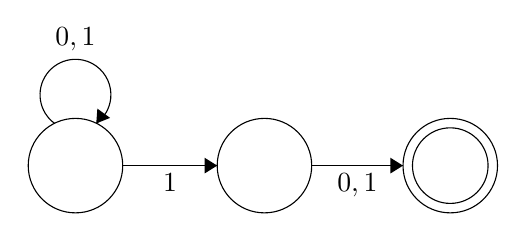
\begin{tikzpicture}[scale=0.2]
\tikzstyle{every node}+=[inner sep=0pt]
\draw [black] (9.2,-22.8) circle (3);
\draw [black] (21.2,-22.8) circle (3);
\draw [black] (33,-22.8) circle (3);
\draw [black] (33,-22.8) circle (2.4);
\draw [black] (12.2,-22.8) -- (18.2,-22.8);
\fill [black] (18.2,-22.8) -- (17.4,-22.3) -- (17.4,-23.3);
\draw (15.2,-23.3) node [below] {$1$};
\draw [black] (24.2,-22.8) -- (30,-22.8);
\fill [black] (30,-22.8) -- (29.2,-22.3) -- (29.2,-23.3);
\draw (27.1,-23.3) node [below] {$0,1$};
\draw [black] (7.877,-20.12) arc (234:-54:2.25);
\draw (9.2,-15.55) node [above] {$0,1$};
\fill [black] (10.52,-20.12) -- (11.4,-19.77) -- (10.59,-19.18);
\end{tikzpicture}
\end{center}

\end{beispiel}

\begin{ubung}[Aufgabe 1]

\begin{enumerate}[a)]
\item
$a+b$:
\begin{center}
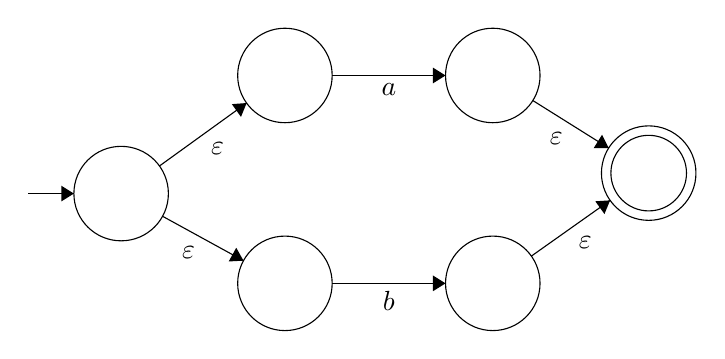
\begin{tikzpicture}[scale=0.2]
\tikzstyle{every node}+=[inner sep=0pt]
\draw [black] (12.7,-24.3) circle (3);
\draw [black] (23.1,-16.8) circle (3);
\draw [black] (36.3,-16.8) circle (3);
\draw [black] (23.1,-30) circle (3);
\draw [black] (36.3,-30) circle (3);
\draw [black] (46.2,-23) circle (3);
\draw [black] (46.2,-23) circle (2.4);
\draw [black] (26.1,-16.8) -- (33.3,-16.8);
\fill [black] (33.3,-16.8) -- (32.5,-16.3) -- (32.5,-17.3);
\draw (29.7,-17.3) node [below] {$a$};
\draw [black] (26.1,-30) -- (33.3,-30);
\fill [black] (33.3,-30) -- (32.5,-29.5) -- (32.5,-30.5);
\draw (29.7,-30.5) node [below] {$b$};
\draw [black] (15.13,-22.55) -- (20.67,-18.55);
\fill [black] (20.67,-18.55) -- (19.73,-18.62) -- (20.31,-19.43);
\draw (18.82,-21.05) node [below] {$\varepsilon$};
\draw [black] (15.33,-25.74) -- (20.47,-28.56);
\fill [black] (20.47,-28.56) -- (20.01,-27.74) -- (19.53,-28.61);
\draw (16.98,-27.65) node [below] {$\varepsilon$};
\draw [black] (38.84,-18.39) -- (43.66,-21.41);
\fill [black] (43.66,-21.41) -- (43.24,-20.56) -- (42.71,-21.41);
\draw (40.33,-20.4) node [below] {$\varepsilon$};
\draw [black] (38.75,-28.27) -- (43.75,-24.73);
\fill [black] (43.75,-24.73) -- (42.81,-24.79) -- (43.39,-25.6);
\draw (42.17,-27) node [below] {$\varepsilon$};
\draw [black] (6.8,-24.3) -- (9.7,-24.3);
\fill [black] (9.7,-24.3) -- (8.9,-23.8) -- (8.9,-24.8);
\end{tikzpicture}
\end{center}

$(a+b)^*$:

\begin{center}
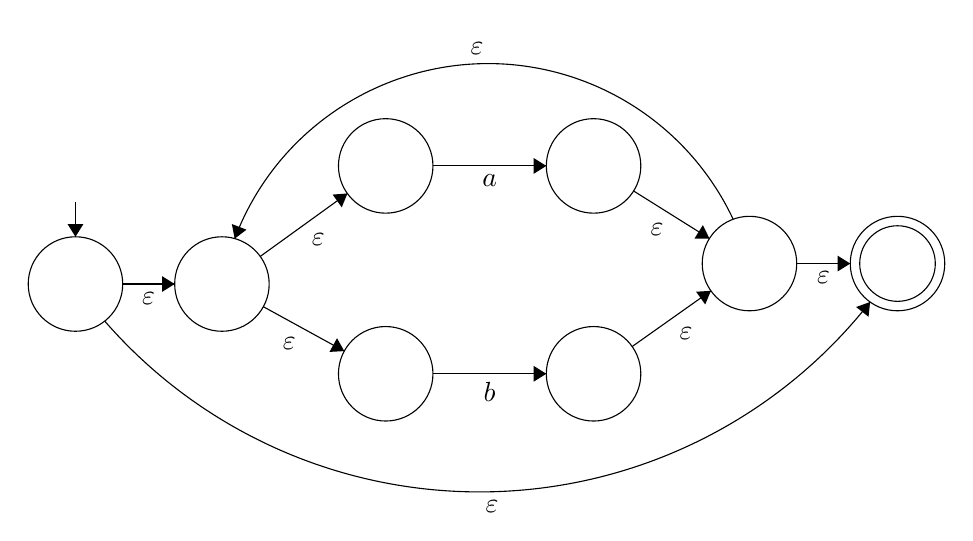
\begin{tikzpicture}[scale=0.2]
\tikzstyle{every node}+=[inner sep=0pt]
\draw [black] (12.7,-24.3) circle (3);
\draw [black] (23.1,-16.8) circle (3);
\draw [black] (36.3,-16.8) circle (3);
\draw [black] (23.1,-30) circle (3);
\draw [black] (36.3,-30) circle (3);
\draw [black] (46.2,-23) circle (3);
\draw [black] (3.4,-24.3) circle (3);
\draw [black] (55.6,-23) circle (3);
\draw [black] (55.6,-23) circle (2.4);
\draw [black] (26.1,-16.8) -- (33.3,-16.8);
\fill [black] (33.3,-16.8) -- (32.5,-16.3) -- (32.5,-17.3);
\draw (29.7,-17.3) node [below] {$a$};
\draw [black] (26.1,-30) -- (33.3,-30);
\fill [black] (33.3,-30) -- (32.5,-29.5) -- (32.5,-30.5);
\draw (29.7,-30.5) node [below] {$b$};
\draw [black] (15.13,-22.55) -- (20.67,-18.55);
\fill [black] (20.67,-18.55) -- (19.73,-18.62) -- (20.31,-19.43);
\draw (18.82,-21.05) node [below] {$\varepsilon$};
\draw [black] (15.33,-25.74) -- (20.47,-28.56);
\fill [black] (20.47,-28.56) -- (20.01,-27.74) -- (19.53,-28.61);
\draw (16.98,-27.65) node [below] {$\varepsilon$};
\draw [black] (38.84,-18.39) -- (43.66,-21.41);
\fill [black] (43.66,-21.41) -- (43.24,-20.56) -- (42.71,-21.41);
\draw (40.33,-20.4) node [below] {$\varepsilon$};
\draw [black] (38.75,-28.27) -- (43.75,-24.73);
\fill [black] (43.75,-24.73) -- (42.81,-24.79) -- (43.39,-25.6);
\draw (42.17,-27) node [below] {$\varepsilon$};
\draw [black] (6.4,-24.3) -- (9.7,-24.3);
\fill [black] (9.7,-24.3) -- (8.9,-23.8) -- (8.9,-24.8);
\draw (8.05,-24.8) node [below] {$\varepsilon$};
\draw [black] (49.2,-23) -- (52.6,-23);
\fill [black] (52.6,-23) -- (51.8,-22.5) -- (51.8,-23.5);
\draw (50.9,-23.5) node [below] {$\varepsilon$};
\draw [black] (13.513,-21.416) arc (159.26273:25.18188:17.201);
\fill [black] (13.51,-21.42) -- (14.26,-20.85) -- (13.33,-20.49);
\draw (28.9,-9.78) node [above] {$\varepsilon$};
\draw [black] (53.862,-25.444) arc (-38.14839:-138.99839:31.539);
\fill [black] (53.86,-25.44) -- (52.97,-25.76) -- (53.76,-26.38);
\draw (29.86,-38.01) node [below] {$\varepsilon$};
\draw [black] (3.4,-19.1) -- (3.4,-21.3);
\fill [black] (3.4,-21.3) -- (3.9,-20.5) -- (2.9,-20.5);
\end{tikzpicture}
\end{center}

$(a+b)^*a$

\begin{center}
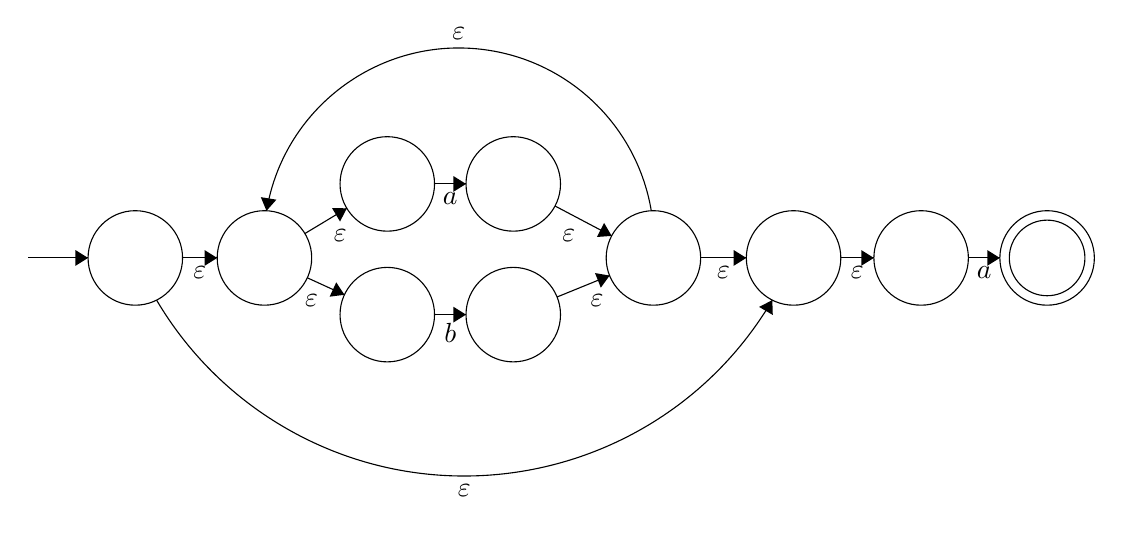
\begin{tikzpicture}[scale=0.2]
\tikzstyle{every node}+=[inner sep=0pt]
\draw [black] (20.5,-24.3) circle (3);
\draw [black] (28.3,-19.6) circle (3);
\draw [black] (36.3,-19.6) circle (3);
\draw [black] (28.3,-27.9) circle (3);
\draw [black] (36.3,-27.9) circle (3);
\draw [black] (45.2,-24.3) circle (3);
\draw [black] (12.3,-24.3) circle (3);
\draw [black] (54.1,-24.3) circle (3);
\draw [black] (62.2,-24.3) circle (3);
\draw [black] (70.2,-24.3) circle (3);
\draw [black] (70.2,-24.3) circle (2.4);
\draw [black] (31.3,-19.6) -- (33.3,-19.6);
\fill [black] (33.3,-19.6) -- (32.5,-19.1) -- (32.5,-20.1);
\draw (32.3,-20.1) node [below] {$a$};
\draw [black] (31.3,-27.9) -- (33.3,-27.9);
\fill [black] (33.3,-27.9) -- (32.5,-27.4) -- (32.5,-28.4);
\draw (32.3,-28.4) node [below] {$b$};
\draw [black] (23.07,-22.75) -- (25.73,-21.15);
\fill [black] (25.73,-21.15) -- (24.79,-21.13) -- (25.3,-21.99);
\draw (25.32,-22.45) node [below] {$\varepsilon$};
\draw [black] (23.22,-25.56) -- (25.58,-26.64);
\fill [black] (25.58,-26.64) -- (25.06,-25.85) -- (24.64,-26.76);
\draw (23.5,-26.61) node [below] {$\varepsilon$};
\draw [black] (38.95,-21) -- (42.55,-22.9);
\fill [black] (42.55,-22.9) -- (42.07,-22.08) -- (41.61,-22.97);
\draw (39.83,-22.45) node [below] {$\varepsilon$};
\draw [black] (39.08,-26.78) -- (42.42,-25.42);
\fill [black] (42.42,-25.42) -- (41.49,-25.26) -- (41.86,-26.19);
\draw (41.63,-26.62) node [below] {$\varepsilon$};
\draw [black] (15.3,-24.3) -- (17.5,-24.3);
\fill [black] (17.5,-24.3) -- (16.7,-23.8) -- (16.7,-24.8);
\draw (16.4,-24.8) node [below] {$\varepsilon$};
\draw [black] (48.2,-24.3) -- (51.1,-24.3);
\fill [black] (51.1,-24.3) -- (50.3,-23.8) -- (50.3,-24.8);
\draw (49.65,-24.8) node [below] {$\varepsilon$};
\draw [black] (20.634,-21.31) arc (-189.49667:-350.50333:12.386);
\fill [black] (20.63,-21.31) -- (21.26,-20.6) -- (20.27,-20.44);
\draw (32.85,-10.47) node [above] {$\varepsilon$};
\draw [black] (52.751,-26.977) arc (-30.52907:-149.47093:22.698);
\fill [black] (52.75,-26.98) -- (51.91,-27.41) -- (52.78,-27.92);
\draw (33.2,-38.64) node [below] {$\varepsilon$};
\draw [black] (65.2,-24.3) -- (67.2,-24.3);
\fill [black] (67.2,-24.3) -- (66.4,-23.8) -- (66.4,-24.8);
\draw (66.2,-24.8) node [below] {$a$};
\draw [black] (57.1,-24.3) -- (59.2,-24.3);
\fill [black] (59.2,-24.3) -- (58.4,-23.8) -- (58.4,-24.8);
\draw (58.15,-24.8) node [below] {$\varepsilon$};
\draw [black] (5.5,-24.3) -- (9.3,-24.3);
\fill [black] (9.3,-24.3) -- (8.5,-23.8) -- (8.5,-24.8);
\end{tikzpicture}
\end{center}

$((a+b)^*a)^*$


\begin{center}
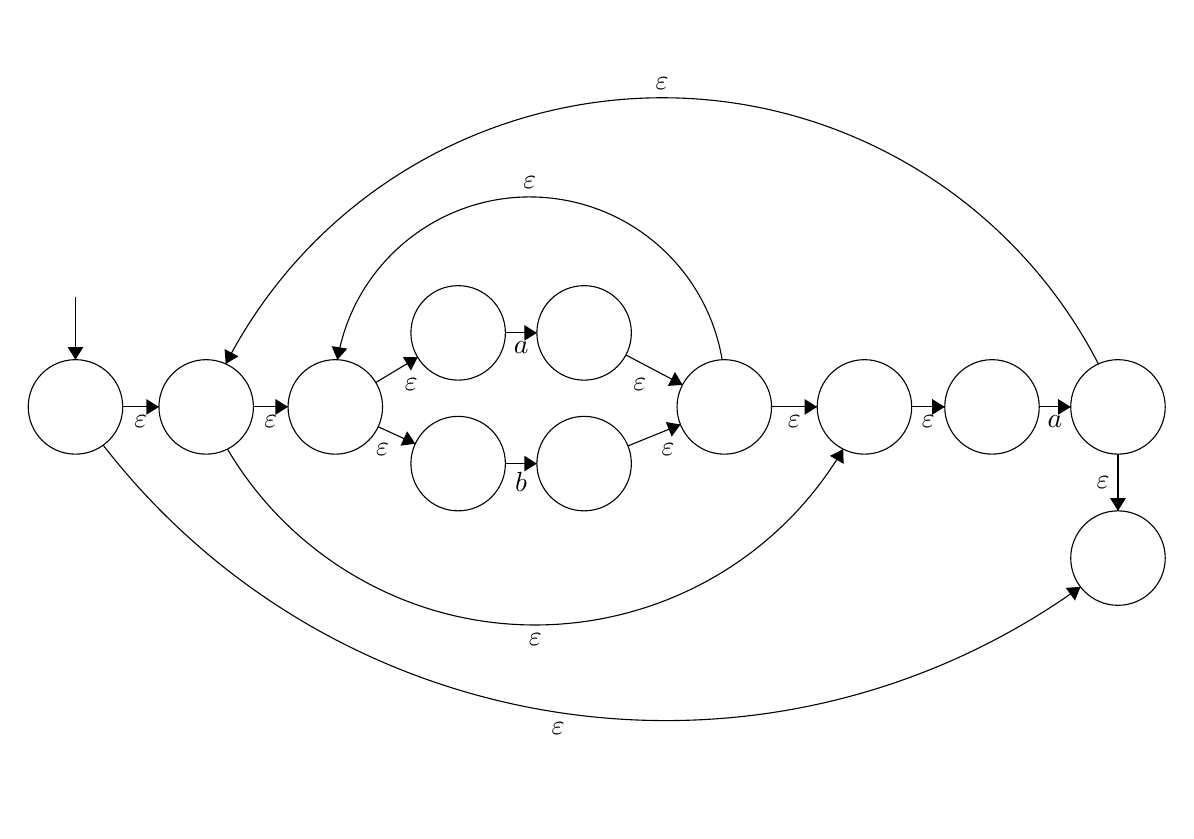
\begin{tikzpicture}[scale=0.2]
\tikzstyle{every node}+=[inner sep=0pt]
\draw [black] (20.5,-24.3) circle (3);
\draw [black] (28.3,-19.6) circle (3);
\draw [black] (36.3,-19.6) circle (3);
\draw [black] (28.3,-27.9) circle (3);
\draw [black] (36.3,-27.9) circle (3);
\draw [black] (45.2,-24.3) circle (3);
\draw [black] (12.3,-24.3) circle (3);
\draw [black] (54.1,-24.3) circle (3);
\draw [black] (62.2,-24.3) circle (3);
\draw [black] (70.2,-24.3) circle (3);
\draw [black] (70.2,-33.9) circle (3);
\draw [black] (4,-24.3) circle (3);
\draw [black] (31.3,-19.6) -- (33.3,-19.6);
\fill [black] (33.3,-19.6) -- (32.5,-19.1) -- (32.5,-20.1);
\draw (32.3,-20.1) node [below] {$a$};
\draw [black] (31.3,-27.9) -- (33.3,-27.9);
\fill [black] (33.3,-27.9) -- (32.5,-27.4) -- (32.5,-28.4);
\draw (32.3,-28.4) node [below] {$b$};
\draw [black] (23.07,-22.75) -- (25.73,-21.15);
\fill [black] (25.73,-21.15) -- (24.79,-21.13) -- (25.3,-21.99);
\draw (25.32,-22.45) node [below] {$\varepsilon$};
\draw [black] (23.22,-25.56) -- (25.58,-26.64);
\fill [black] (25.58,-26.64) -- (25.06,-25.85) -- (24.64,-26.76);
\draw (23.5,-26.61) node [below] {$\varepsilon$};
\draw [black] (38.95,-21) -- (42.55,-22.9);
\fill [black] (42.55,-22.9) -- (42.07,-22.08) -- (41.61,-22.97);
\draw (39.83,-22.45) node [below] {$\varepsilon$};
\draw [black] (39.08,-26.78) -- (42.42,-25.42);
\fill [black] (42.42,-25.42) -- (41.49,-25.26) -- (41.86,-26.19);
\draw (41.63,-26.62) node [below] {$\varepsilon$};
\draw [black] (15.3,-24.3) -- (17.5,-24.3);
\fill [black] (17.5,-24.3) -- (16.7,-23.8) -- (16.7,-24.8);
\draw (16.4,-24.8) node [below] {$\varepsilon$};
\draw [black] (48.2,-24.3) -- (51.1,-24.3);
\fill [black] (51.1,-24.3) -- (50.3,-23.8) -- (50.3,-24.8);
\draw (49.65,-24.8) node [below] {$\varepsilon$};
\draw [black] (20.634,-21.31) arc (-189.49667:-350.50333:12.386);
\fill [black] (20.63,-21.31) -- (21.26,-20.6) -- (20.27,-20.44);
\draw (32.85,-10.47) node [above] {$\varepsilon$};
\draw [black] (52.751,-26.977) arc (-30.52907:-149.47093:22.698);
\fill [black] (52.75,-26.98) -- (51.91,-27.41) -- (52.78,-27.92);
\draw (33.2,-38.64) node [below] {$\varepsilon$};
\draw [black] (65.2,-24.3) -- (67.2,-24.3);
\fill [black] (67.2,-24.3) -- (66.4,-23.8) -- (66.4,-24.8);
\draw (66.2,-24.8) node [below] {$a$};
\draw [black] (57.1,-24.3) -- (59.2,-24.3);
\fill [black] (59.2,-24.3) -- (58.4,-23.8) -- (58.4,-24.8);
\draw (58.15,-24.8) node [below] {$\varepsilon$};
\draw [black] (13.543,-21.571) arc (152.75003:27.24997:31.166);
\fill [black] (13.54,-21.57) -- (14.35,-21.09) -- (13.47,-20.63);
\draw (41.25,-4.18) node [above] {$\varepsilon$};
\draw [black] (70.2,-27.3) -- (70.2,-30.9);
\fill [black] (70.2,-30.9) -- (70.7,-30.1) -- (69.7,-30.1);
\draw (69.7,-29.1) node [left] {$\varepsilon$};
\draw [black] (7,-24.3) -- (9.3,-24.3);
\fill [black] (9.3,-24.3) -- (8.5,-23.8) -- (8.5,-24.8);
\draw (8.15,-24.8) node [below] {$\varepsilon$};
\draw [black] (4,-17.3) -- (4,-21.3);
\fill [black] (4,-21.3) -- (4.5,-20.5) -- (3.5,-20.5);
\draw [black] (67.823,-35.73) arc (-54.30569:-142.19678:45.185);
\fill [black] (67.82,-35.73) -- (66.88,-35.79) -- (67.47,-36.6);
\draw (34.65,-44.34) node [below] {$\varepsilon$};
\end{tikzpicture}
\end{center}

\item $a+b$

\begin{center}
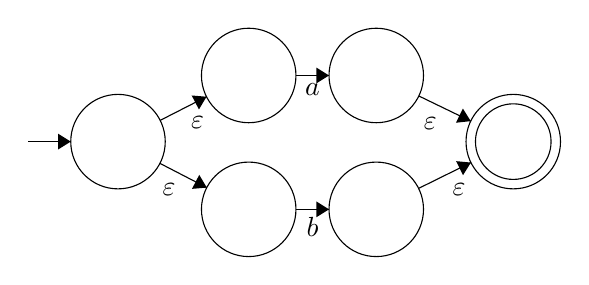
\begin{tikzpicture}[scale=0.2]
\tikzstyle{every node}+=[inner sep=0pt]
\draw [black] (32.4,-24.2) circle (3);
\draw [black] (40.5,-24.2) circle (3);
\draw [black] (32.4,-32.7) circle (3);
\draw [black] (40.5,-32.7) circle (3);
\draw [black] (24.1,-28.4) circle (3);
\draw [black] (49.2,-28.4) circle (3);
\draw [black] (49.2,-28.4) circle (2.4);
\draw [black] (35.4,-24.2) -- (37.5,-24.2);
\fill [black] (37.5,-24.2) -- (36.7,-23.7) -- (36.7,-24.7);
\draw (36.45,-24.7) node [below] {$a$};
\draw [black] (35.4,-32.7) -- (37.5,-32.7);
\fill [black] (37.5,-32.7) -- (36.7,-32.2) -- (36.7,-33.2);
\draw (36.45,-33.2) node [below] {$b$};
\draw [black] (26.78,-27.05) -- (29.72,-25.55);
\fill [black] (29.72,-25.55) -- (28.78,-25.47) -- (29.24,-26.36);
\draw (29.16,-26.8) node [below] {$\varepsilon$};
\draw [black] (26.76,-29.78) -- (29.74,-31.32);
\fill [black] (29.74,-31.32) -- (29.26,-30.51) -- (28.8,-31.4);
\draw (27.34,-31.05) node [below] {$\varepsilon$};
\draw [black] (43.2,-25.5) -- (46.5,-27.1);
\fill [black] (46.5,-27.1) -- (46,-26.3) -- (45.56,-27.2);
\draw (43.94,-26.81) node [below] {$\varepsilon$};
\draw [black] (43.19,-31.37) -- (46.51,-29.73);
\fill [black] (46.51,-29.73) -- (45.57,-29.64) -- (46.01,-30.53);
\draw (45.76,-31.05) node [below] {$\varepsilon$};
\draw [black] (18.4,-28.4) -- (21.1,-28.4);
\fill [black] (21.1,-28.4) -- (20.3,-27.9) -- (20.3,-28.9);
\end{tikzpicture}
\end{center}

$a+b+c$

\begin{center}
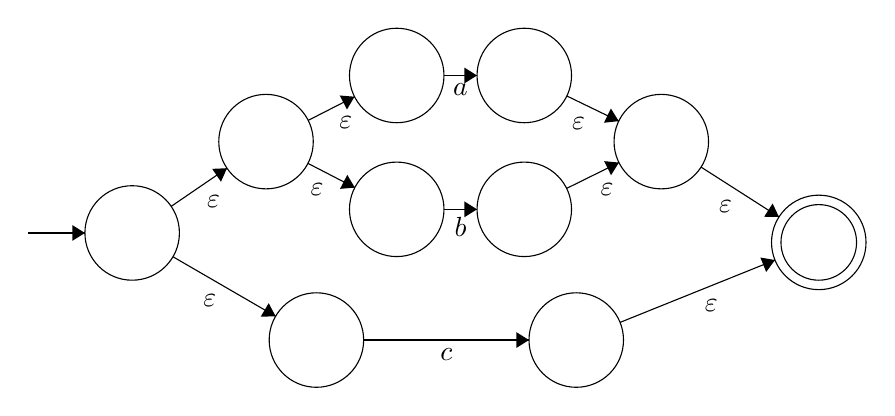
\begin{tikzpicture}[scale=0.2]
\tikzstyle{every node}+=[inner sep=0pt]
\draw [black] (32.4,-24.2) circle (3);
\draw [black] (40.5,-24.2) circle (3);
\draw [black] (32.4,-32.7) circle (3);
\draw [black] (40.5,-32.7) circle (3);
\draw [black] (24.1,-28.4) circle (3);
\draw [black] (49.2,-28.4) circle (3);
\draw [black] (15.6,-34.2) circle (3);
\draw [black] (27.3,-41) circle (3);
\draw [black] (43.8,-41) circle (3);
\draw [black] (59.2,-34.8) circle (3);
\draw [black] (59.2,-34.8) circle (2.4);
\draw [black] (35.4,-24.2) -- (37.5,-24.2);
\fill [black] (37.5,-24.2) -- (36.7,-23.7) -- (36.7,-24.7);
\draw (36.45,-24.7) node [below] {$a$};
\draw [black] (35.4,-32.7) -- (37.5,-32.7);
\fill [black] (37.5,-32.7) -- (36.7,-32.2) -- (36.7,-33.2);
\draw (36.45,-33.2) node [below] {$b$};
\draw [black] (26.78,-27.05) -- (29.72,-25.55);
\fill [black] (29.72,-25.55) -- (28.78,-25.47) -- (29.24,-26.36);
\draw (29.16,-26.8) node [below] {$\varepsilon$};
\draw [black] (26.76,-29.78) -- (29.74,-31.32);
\fill [black] (29.74,-31.32) -- (29.26,-30.51) -- (28.8,-31.4);
\draw (27.34,-31.05) node [below] {$\varepsilon$};
\draw [black] (43.2,-25.5) -- (46.5,-27.1);
\fill [black] (46.5,-27.1) -- (46,-26.3) -- (45.56,-27.2);
\draw (43.94,-26.81) node [below] {$\varepsilon$};
\draw [black] (43.19,-31.37) -- (46.51,-29.73);
\fill [black] (46.51,-29.73) -- (45.57,-29.64) -- (46.01,-30.53);
\draw (45.76,-31.05) node [below] {$\varepsilon$};
\draw [black] (18.08,-32.51) -- (21.62,-30.09);
\fill [black] (21.62,-30.09) -- (20.68,-30.13) -- (21.24,-30.95);
\draw (20.77,-31.8) node [below] {$\varepsilon$};
\draw [black] (30.3,-41) -- (40.8,-41);
\fill [black] (40.8,-41) -- (40,-40.5) -- (40,-41.5);
\draw (35.55,-41.5) node [below] {$c$};
\draw [black] (18.19,-35.71) -- (24.71,-39.49);
\fill [black] (24.71,-39.49) -- (24.27,-38.66) -- (23.76,-39.52);
\draw (20.53,-38.1) node [below] {$\varepsilon$};
\draw [black] (46.58,-39.88) -- (56.42,-35.92);
\fill [black] (56.42,-35.92) -- (55.49,-35.76) -- (55.86,-36.68);
\draw (52.38,-38.42) node [below] {$\varepsilon$};
\draw [black] (51.73,-30.02) -- (56.67,-33.18);
\fill [black] (56.67,-33.18) -- (56.27,-32.33) -- (55.73,-33.17);
\draw (53.28,-32.1) node [below] {$\varepsilon$};
\draw [black] (9,-34.2) -- (12.6,-34.2);
\fill [black] (12.6,-34.2) -- (11.8,-33.7) -- (11.8,-34.7);
\end{tikzpicture}
\end{center}

$(a+b+c)\cdot (a+b)$

\begin{center}
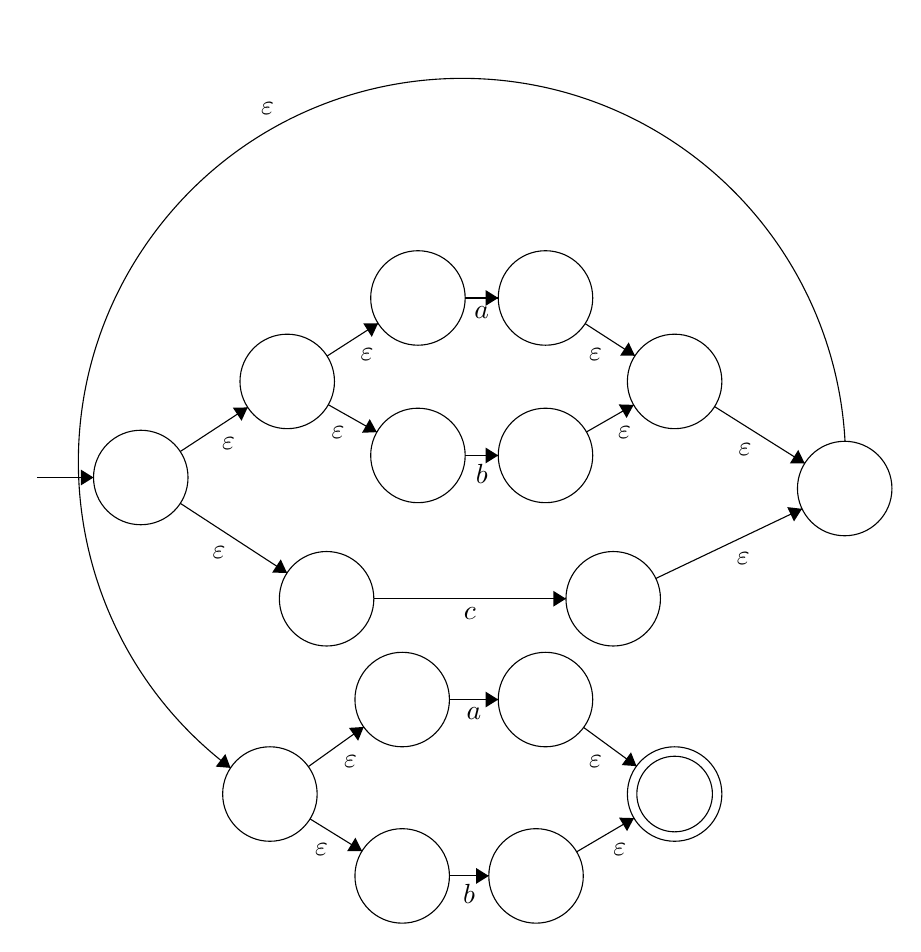
\begin{tikzpicture}[scale=0.2]
\tikzstyle{every node}+=[inner sep=0pt]
\draw [black] (32.4,-15.7) circle (3);
\draw [black] (40.5,-15.7) circle (3);
\draw [black] (32.4,-25.7) circle (3);
\draw [black] (40.5,-25.7) circle (3);
\draw [black] (24.1,-21) circle (3);
\draw [black] (48.7,-21) circle (3);
\draw [black] (14.8,-27.1) circle (3);
\draw [black] (26.6,-34.8) circle (3);
\draw [black] (44.8,-34.8) circle (3);
\draw [black] (59.5,-27.8) circle (3);
\draw [black] (23,-47.2) circle (3);
\draw [black] (31.4,-41.2) circle (3);
\draw [black] (40.5,-41.2) circle (3);
\draw [black] (31.4,-52.4) circle (3);
\draw [black] (39.9,-52.4) circle (3);
\draw [black] (48.7,-47.2) circle (3);
\draw [black] (48.7,-47.2) circle (2.4);
\draw [black] (35.4,-15.7) -- (37.5,-15.7);
\fill [black] (37.5,-15.7) -- (36.7,-15.2) -- (36.7,-16.2);
\draw (36.45,-16.2) node [below] {$a$};
\draw [black] (35.4,-25.7) -- (37.5,-25.7);
\fill [black] (37.5,-25.7) -- (36.7,-25.2) -- (36.7,-26.2);
\draw (36.45,-26.2) node [below] {$b$};
\draw [black] (26.63,-19.39) -- (29.87,-17.31);
\fill [black] (29.87,-17.31) -- (28.93,-17.32) -- (29.47,-18.17);
\draw (29.17,-18.85) node [below] {$\varepsilon$};
\draw [black] (26.71,-22.48) -- (29.79,-24.22);
\fill [black] (29.79,-24.22) -- (29.34,-23.39) -- (28.85,-24.26);
\draw (27.33,-23.85) node [below] {$\varepsilon$};
\draw [black] (43.02,-17.33) -- (46.18,-19.37);
\fill [black] (46.18,-19.37) -- (45.78,-18.52) -- (45.24,-19.36);
\draw (43.68,-18.85) node [below] {$\varepsilon$};
\draw [black] (43.1,-24.21) -- (46.1,-22.49);
\fill [black] (46.1,-22.49) -- (45.15,-22.46) -- (45.65,-23.32);
\draw (45.52,-23.85) node [below] {$\varepsilon$};
\draw [black] (17.31,-25.45) -- (21.59,-22.65);
\fill [black] (21.59,-22.65) -- (20.65,-22.67) -- (21.2,-23.5);
\draw (20.37,-24.55) node [below] {$\varepsilon$};
\draw [black] (29.6,-34.8) -- (41.8,-34.8);
\fill [black] (41.8,-34.8) -- (41,-34.3) -- (41,-35.3);
\draw (35.7,-35.3) node [below] {$c$};
\draw [black] (17.31,-28.74) -- (24.09,-33.16);
\fill [black] (24.09,-33.16) -- (23.69,-32.3) -- (23.14,-33.14);
\draw (19.78,-31.45) node [below] {$\varepsilon$};
\draw [black] (47.51,-33.51) -- (56.79,-29.09);
\fill [black] (56.79,-29.09) -- (55.85,-28.98) -- (56.28,-29.89);
\draw (53.06,-31.81) node [below] {$\varepsilon$};
\draw [black] (51.24,-22.6) -- (56.96,-26.2);
\fill [black] (56.96,-26.2) -- (56.55,-25.35) -- (56.02,-26.2);
\draw (53.18,-24.9) node [below] {$\varepsilon$};
\draw [black] (8.2,-27.1) -- (11.8,-27.1);
\fill [black] (11.8,-27.1) -- (11,-26.6) -- (11,-27.6);
\draw [black] (34.4,-41.2) -- (37.5,-41.2);
\fill [black] (37.5,-41.2) -- (36.7,-40.7) -- (36.7,-41.7);
\draw (35.95,-41.7) node [below] {$a$};
\draw [black] (34.4,-52.4) -- (36.9,-52.4);
\fill [black] (36.9,-52.4) -- (36.1,-51.9) -- (36.1,-52.9);
\draw (35.65,-52.9) node [below] {$b$};
\draw [black] (25.44,-45.46) -- (28.96,-42.94);
\fill [black] (28.96,-42.94) -- (28.02,-43) -- (28.6,-43.82);
\draw (28.12,-44.7) node [below] {$\varepsilon$};
\draw [black] (25.55,-48.78) -- (28.85,-50.82);
\fill [black] (28.85,-50.82) -- (28.43,-49.97) -- (27.91,-50.82);
\draw (26.28,-50.3) node [below] {$\varepsilon$};
\draw [black] (42.92,-42.97) -- (46.28,-45.43);
\fill [black] (46.28,-45.43) -- (45.93,-44.55) -- (45.34,-45.36);
\draw (43.68,-44.7) node [below] {$\varepsilon$};
\draw [black] (42.48,-50.87) -- (46.12,-48.73);
\fill [black] (46.12,-48.73) -- (45.17,-48.7) -- (45.68,-49.56);
\draw (45.22,-50.3) node [below] {$\varepsilon$};
\draw [black] (20.502,-45.542) arc (-127.10424:-356.91386:24.36);
\fill [black] (20.5,-45.54) -- (20.17,-44.66) -- (19.56,-45.46);
\draw (22.85,-4.1) node [above] {$\varepsilon$};
\end{tikzpicture}
\end{center}

Letzter Schritt:

\begin{center}
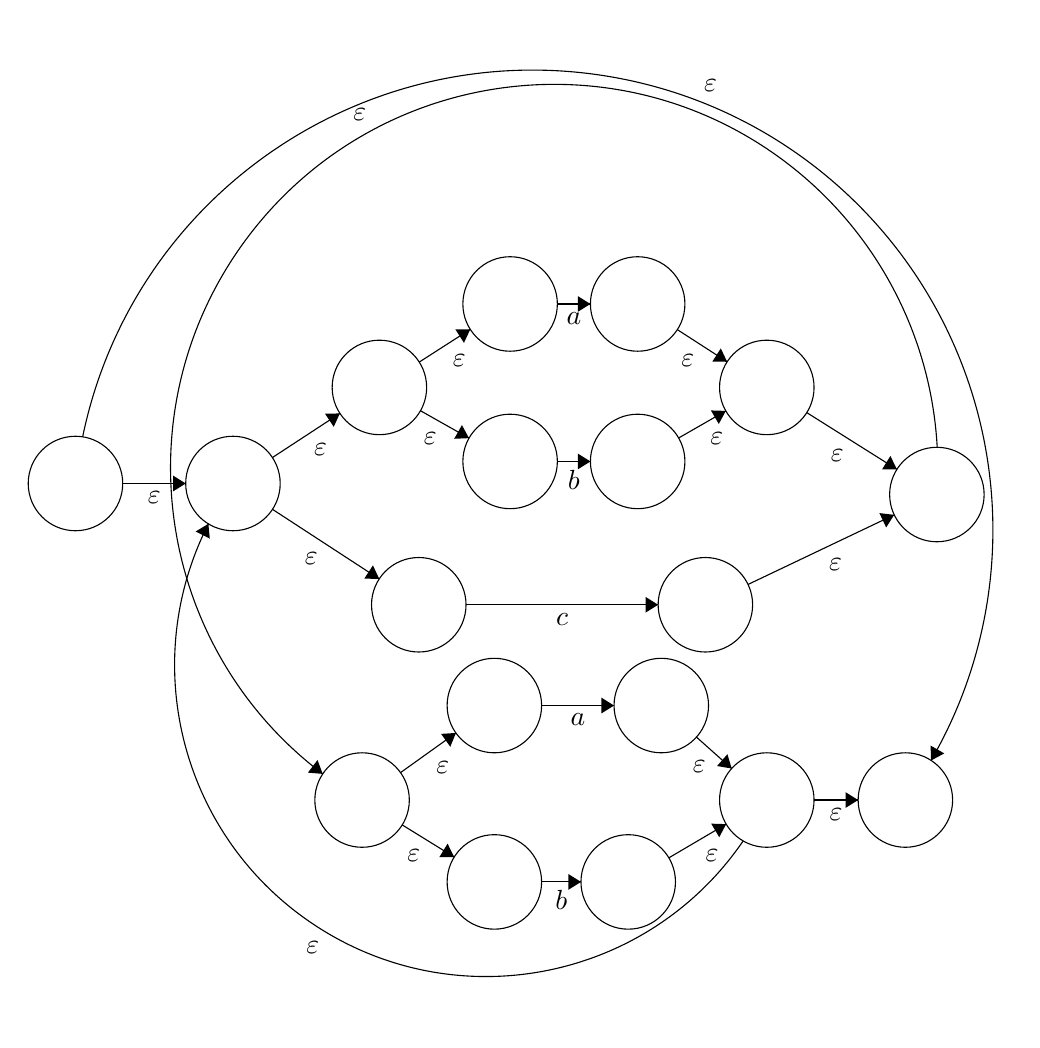
\begin{tikzpicture}[scale=0.2]
\tikzstyle{every node}+=[inner sep=0pt]
\draw [black] (32.4,-15.7) circle (3);
\draw [black] (40.5,-15.7) circle (3);
\draw [black] (32.4,-25.7) circle (3);
\draw [black] (40.5,-25.7) circle (3);
\draw [black] (24.1,-21) circle (3);
\draw [black] (48.7,-21) circle (3);
\draw [black] (14.8,-27.1) circle (3);
\draw [black] (26.6,-34.8) circle (3);
\draw [black] (44.8,-34.8) circle (3);
\draw [black] (59.5,-27.8) circle (3);
\draw [black] (23,-47.2) circle (3);
\draw [black] (31.4,-41.2) circle (3);
\draw [black] (42,-41.2) circle (3);
\draw [black] (31.4,-52.4) circle (3);
\draw [black] (39.9,-52.4) circle (3);
\draw [black] (48.7,-47.2) circle (3);
\draw [black] (57.5,-47.2) circle (3);
\draw [black] (4.8,-27.1) circle (3);
\draw [black] (35.4,-15.7) -- (37.5,-15.7);
\fill [black] (37.5,-15.7) -- (36.7,-15.2) -- (36.7,-16.2);
\draw (36.45,-16.2) node [below] {$a$};
\draw [black] (35.4,-25.7) -- (37.5,-25.7);
\fill [black] (37.5,-25.7) -- (36.7,-25.2) -- (36.7,-26.2);
\draw (36.45,-26.2) node [below] {$b$};
\draw [black] (26.63,-19.39) -- (29.87,-17.31);
\fill [black] (29.87,-17.31) -- (28.93,-17.32) -- (29.47,-18.17);
\draw (29.17,-18.85) node [below] {$\varepsilon$};
\draw [black] (26.71,-22.48) -- (29.79,-24.22);
\fill [black] (29.79,-24.22) -- (29.34,-23.39) -- (28.85,-24.26);
\draw (27.33,-23.85) node [below] {$\varepsilon$};
\draw [black] (43.02,-17.33) -- (46.18,-19.37);
\fill [black] (46.18,-19.37) -- (45.78,-18.52) -- (45.24,-19.36);
\draw (43.68,-18.85) node [below] {$\varepsilon$};
\draw [black] (43.1,-24.21) -- (46.1,-22.49);
\fill [black] (46.1,-22.49) -- (45.15,-22.46) -- (45.65,-23.32);
\draw (45.52,-23.85) node [below] {$\varepsilon$};
\draw [black] (17.31,-25.45) -- (21.59,-22.65);
\fill [black] (21.59,-22.65) -- (20.65,-22.67) -- (21.2,-23.5);
\draw (20.37,-24.55) node [below] {$\varepsilon$};
\draw [black] (29.6,-34.8) -- (41.8,-34.8);
\fill [black] (41.8,-34.8) -- (41,-34.3) -- (41,-35.3);
\draw (35.7,-35.3) node [below] {$c$};
\draw [black] (17.31,-28.74) -- (24.09,-33.16);
\fill [black] (24.09,-33.16) -- (23.69,-32.3) -- (23.14,-33.14);
\draw (19.78,-31.45) node [below] {$\varepsilon$};
\draw [black] (47.51,-33.51) -- (56.79,-29.09);
\fill [black] (56.79,-29.09) -- (55.85,-28.98) -- (56.28,-29.89);
\draw (53.06,-31.81) node [below] {$\varepsilon$};
\draw [black] (51.24,-22.6) -- (56.96,-26.2);
\fill [black] (56.96,-26.2) -- (56.55,-25.35) -- (56.02,-26.2);
\draw (53.18,-24.9) node [below] {$\varepsilon$};
\draw [black] (34.4,-41.2) -- (39,-41.2);
\fill [black] (39,-41.2) -- (38.2,-40.7) -- (38.2,-41.7);
\draw (36.7,-41.7) node [below] {$a$};
\draw [black] (34.4,-52.4) -- (36.9,-52.4);
\fill [black] (36.9,-52.4) -- (36.1,-51.9) -- (36.1,-52.9);
\draw (35.65,-52.9) node [below] {$b$};
\draw [black] (25.44,-45.46) -- (28.96,-42.94);
\fill [black] (28.96,-42.94) -- (28.02,-43) -- (28.6,-43.82);
\draw (28.12,-44.7) node [below] {$\varepsilon$};
\draw [black] (25.55,-48.78) -- (28.85,-50.82);
\fill [black] (28.85,-50.82) -- (28.43,-49.97) -- (27.91,-50.82);
\draw (26.28,-50.3) node [below] {$\varepsilon$};
\draw [black] (44.23,-43.2) -- (46.47,-45.2);
\fill [black] (46.47,-45.2) -- (46.2,-44.29) -- (45.54,-45.04);
\draw (44.42,-44.69) node [below] {$\varepsilon$};
\draw [black] (42.48,-50.87) -- (46.12,-48.73);
\fill [black] (46.12,-48.73) -- (45.17,-48.7) -- (45.68,-49.56);
\draw (45.22,-50.3) node [below] {$\varepsilon$};
\draw [black] (20.502,-45.542) arc (-127.10424:-356.91386:24.36);
\fill [black] (20.5,-45.54) -- (20.17,-44.66) -- (19.56,-45.46);
\draw (22.85,-4.1) node [above] {$\varepsilon$};
\draw [black] (51.7,-47.2) -- (54.5,-47.2);
\fill [black] (54.5,-47.2) -- (53.7,-46.7) -- (53.7,-47.7);
\draw (53.1,-47.7) node [below] {$\varepsilon$};
\draw [black] (7.8,-27.1) -- (11.8,-27.1);
\fill [black] (11.8,-27.1) -- (11,-26.6) -- (11,-27.6);
\draw (9.8,-27.6) node [below] {$\varepsilon$};
\draw [black] (47.2,-49.795) arc (-34.37509:-206.95404:19.78);
\fill [black] (13.24,-29.66) -- (12.43,-30.15) -- (13.33,-30.6);
\draw (19.87,-56.14) node [below] {$\varepsilon$};
\draw [black] (5.256,-24.136) arc (168.30285:-30.05697:29.205);
\fill [black] (59.13,-44.69) -- (59.97,-44.24) -- (59.1,-43.74);
\draw (45.13,-2.25) node [above] {$\varepsilon$};
\end{tikzpicture}
\end{center}

\end{enumerate}

\end{ubung}

\begin{proof}[Beweis für 2.]

Idee: Dynamische Programmierung. Die Teilprobleme hier sind: Für jedes Paar $(p,q)$ von Zuständen finde einen regulären Ausdruck, der alle Wörter beschreibt, die von $p$ nach $q$ führen.

Genauer: Sei $A = (Q, \Sigma, \delta, q_0, F)$ ein DEA, seien die Zustände durchnumeriert, d.h. $Q = \{1,2,\dots , n \}$, $q_0 = 1$.

\begin{enumerate}
\item Berechne für alle $i, j \in \{1,2,\dots n\}$ reguläre Ausdrücke $\alpha_{i,j}^{(0)}$, die die direkten Verbindungen von Zustand $i$ zu Zustand $j$ beschreiben:
\begin{enumerate}[a)]
\item $i = j$:
\begin{center}
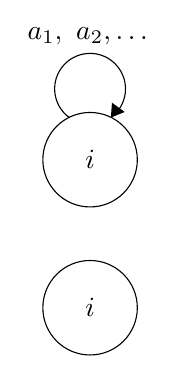
\begin{tikzpicture}[scale=0.2]
\tikzstyle{every node}+=[inner sep=0pt]
\draw [black] (22.5,-20.3) circle (3);
\draw (22.5,-20.3) node {$i$};
\draw [black] (22.5,-29.7) circle (3);
\draw (22.5,-29.7) node {$i$};
\draw [black] (21.177,-17.62) arc (234:-54:2.25);
\draw (22.5,-13.05) node [above] {$a_1,\mbox{ }a_2,\dots$};
\fill [black] (23.82,-17.62) -- (24.7,-17.27) -- (23.89,-16.68);
\end{tikzpicture}
\end{center}

$\alpha_{i,i}^{(0)} = \varepsilon + a_1 + a_2 + \dots$ oder $\alpha_{i,i}^{(0)} = \varepsilon$

\item $i \neq j$

$\alpha_{i,i}^{(0)} = a_1 + a_2 + \dots$ oder $\alpha_{i,j}^{(0)} = \varnothing$
\end{enumerate}

\item Nun werden nacheinander alle anderen Zustände als mögliche Zwischenstation auf dem Weg von $i$ nach $j$ hinzugenommen -- zunächst den Zustand $1$:

$\alpha_{i,j}^{(1)}$ beschreibt die Wörter, mit denen man von $i$ nach $j$ kommt und zwischendurch nur den Zustand $1$ besucht.
\end{enumerate}

\begin{center}
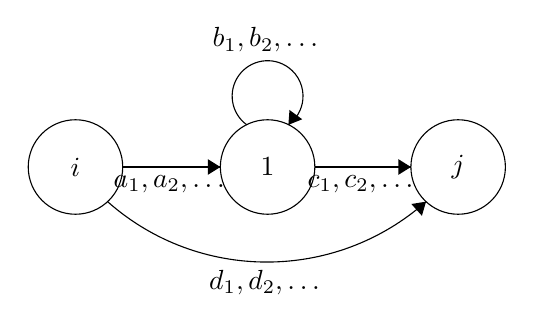
\begin{tikzpicture}[scale=0.2]
\tikzstyle{every node}+=[inner sep=0pt]
\draw [black] (8.9,-14.3) circle (3);
\draw (8.9,-14.3) node {$i$};
\draw [black] (33.2,-14.3) circle (3);
\draw (33.2,-14.3) node {$j$};
\draw [black] (21.1,-14.3) circle (3);
\draw (21.1,-14.3) node {$1$};
\draw [black] (19.777,-11.62) arc (234:-54:2.25);
\draw (21.1,-7.05) node [above] {$b_1,b_2,\dots$};
\fill [black] (22.42,-11.62) -- (23.3,-11.27) -- (22.49,-10.68);
\draw [black] (11.9,-14.3) -- (18.1,-14.3);
\fill [black] (18.1,-14.3) -- (17.3,-13.8) -- (17.3,-14.8);
\draw (15,-14.8) node [below] {$a_1,a_2,\dots$};
\draw [black] (24.1,-14.3) -- (30.2,-14.3);
\fill [black] (30.2,-14.3) -- (29.4,-13.8) -- (29.4,-14.8);
\draw (27.15,-14.8) node [below] {$c_1,c_2,\dots$};
\draw [black] (31.165,-16.498) arc (-48.43714:-131.56286:15.246);
\fill [black] (31.16,-16.5) -- (30.23,-16.65) -- (30.9,-17.4);
\draw (21.05,-20.84) node [below] {$d_1,d_2,\dots$};
\end{tikzpicture}
\end{center}

$\alpha_{i,j}^{(1)} = \alpha_{i,j}^{(0)} + \alpha_{i,1}^{(0)}(\alpha_{1,1}^{(0)})^*\alpha_{1,j}^{(0)} $

Induktion: Wir nehmen an, dass wir $\alpha_{i,j}^{(k-1)}$ für alle $i,j$ schon berechnet haben. Dann gilt: $\alpha_{i,1}^{(k)} = 
\alpha_{i,j}^{(k-1)} + \alpha_{i,k}^{(k-1)}(\alpha_{k,k}^{(k-1)})^* \alpha_{k,j}^{(k-1)}$

Daraus folgt der Reguläre Ausdruck für den DEA $A$ mit $q_0 = 1$ und $F = \{f_1, f_2, \dots f_m \}$:

\[
\alpha_{1,f_1}^{(n)} + \alpha_{1,f_2}^{(n)} + \dots + \alpha_{1,f_m}^{(n)}
\]

\end{proof}

\begin{beispiel}

DEA $A$:

\begin{center}
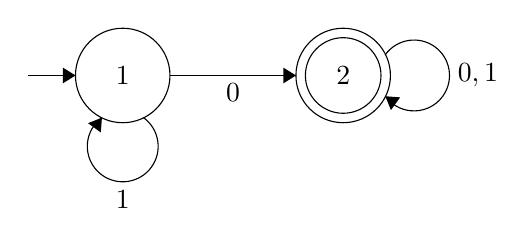
\begin{tikzpicture}[scale=0.2]
\tikzstyle{every node}+=[inner sep=0pt]
\draw [black] (15.7,-17.1) circle (3);
\draw (15.7,-17.1) node {$1$};
\draw [black] (29.7,-17.1) circle (3);
\draw (29.7,-17.1) node {$2$};
\draw [black] (29.7,-17.1) circle (2.4);
\draw [black] (18.7,-17.1) -- (26.7,-17.1);
\fill [black] (26.7,-17.1) -- (25.9,-16.6) -- (25.9,-17.6);
\draw (22.7,-17.6) node [below] {$0$};
\draw [black] (32.38,-15.777) arc (144:-144:2.25);
\draw (36.95,-17.1) node [right] {$0,1$};
\fill [black] (32.38,-18.42) -- (32.73,-19.3) -- (33.32,-18.49);
\draw [black] (17.023,-19.78) arc (54:-234:2.25);
\draw (15.7,-24.35) node [below] {$1$};
\fill [black] (14.38,-19.78) -- (13.5,-20.13) -- (14.31,-20.72);
\draw [black] (9.7,-17.1) -- (12.7,-17.1);
\fill [black] (12.7,-17.1) -- (11.9,-16.6) -- (11.9,-17.6);
\end{tikzpicture}
\end{center}

\begin{enumerate}
\item $\alpha_{1,1}^{(0)} = 1 + \varepsilon$

$\alpha_{1,2}^{(0)} = 1$

$\alpha_{2,1}^{(0)} = \varnothing$

$\alpha_{2,2}^{(0)} = \varepsilon + 0 + 1$

\item $\alpha_{1,1}^{(1)} = \alpha_{1,1}^{(0)} + \alpha_{1,1}^{(0)}(\alpha_{1,1}^{(0)})^*\alpha_{1,1}^{(0)} = 1 + \varepsilon + (1 + \varepsilon)(\alpha_{1,1}^{(0)})^*\alpha_{1,1}^{(0)} = (1+\varepsilon)^* = 1^*$

$\alpha_{1,2}^{(1)} = \alpha_{1,2}^{(0)} +  \alpha_{1,1}^{(0)}( \alpha_{1,1}^{(0)})^* \alpha_{1,2}^{(0)}$
$= 0 + (1+\varepsilon)(1+\varepsilon)^*0 = 1^*0$

$\alpha_{2,1}^{(1)} = \alpha_{2,1}^{(0)}+ \alpha_{2,1}^{(1)}(\alpha_{1,1}^{(1)})^*\alpha_{1,1}^{(1)} = \varnothing + \varnothing(1+\varepsilon)^*(1+\varepsilon) = \varnothing$

$\alpha_{2,2}^{(1)} =\alpha_{2,2}^{(0)} + \alpha_{2,1}^{(0)}(\alpha_{1,1}^{(0)})^*\alpha_{1,2}^{(0)} = (\varepsilon+0+1) + \varnothing \dots = \varepsilon + 0 + 1$

\item $\alpha_{1,1}^{(1)} + \alpha_{1,2}^{(1)}(\alpha_{2,2}^{(1)})^*\alpha_{2,1}^{(1)}
= 1^* + 1^*0 (\varepsilon + 0+1) \varnothing = 1^*$

$\alpha_{1,2}^{(2)} =  \alpha_{1,2}^{(1)} + \alpha_{1,2}^{(1)} (\alpha_{2,2}^{(1)})^* \alpha_{2,2}^{(1)} = 1^*0+1^*0(\varepsilon + 0 + 1)^* (\varepsilon + 0 + 1) = 1^*0(0+1)^* = \mathcal{L}(A) $

\end{enumerate}

\end{beispiel}

\section{Reguläre Sprachen und ihre Eigenschaften}

\begin{definition}[Reguläre Sprache]
Eine Sprache heisst regulär, wenn sie von einem DEA akzeptiert wird.
\[
\mathcal{L}_{\textrm{reg}} = \mathcal{L}(\textrm{DEA}) = \{ L | L \textrm{ist regulär} \}
\]
\end{definition}

Ziel: Charakterisierung von regulären Sprachen.

\subsection{Abschlusseigenschaften regulärer Sprachen}

\begin{description}
\item[Vereinigung] Wenn $L$ und $M$ reguläre Sprachen sind, dann ist auch $L$ vereinigt mit $M$ regulär.
\begin{proof}[Beweis]
Wenn $L$ und $M$ regulär sind, dann existieren reguläre Ausdrücke $\alpha$ und $\beta$ für $L$ und $M$, d.h. $L(\alpha) = L$ und $L(\beta) = M$.

Daraus folgt, dass $\alpha + \beta$ ebenfalls ein RA ist, daraus folgt $L(\alpha + \beta) = L \cup M$ (gemäss Definition der Vereinigung von RA).
\end{proof}

\item[Verkettung] Wenn $L$ und $M$ reguläre Sprachen sind, dann ist auch $L$ verkettet mit $M$ regulär.
\begin{proof}[Beweis]
Analog der Vereinigung.
\end{proof}

\item[Kleene'scher Stern] Wenn $L$ eine reguläre Sprache ist, dann ist auch $L^*$ eine reguläre Sprache.
\begin{proof}[Beweis]
Analog der Vereinigung.
\end{proof}

\item[Komplement] Wenn $L$ eine reguläre Sprache ist, dann ist auch $\bar{L} = \Sigma^* - L$ regulär.

\begin{proof}[Beweis]
Sei $A$ ein DEA für $L$. Dann gibt es für jedes Wort $w$ aus $\Sigma^*$ einen eindeutigen Zustand, in dem der DEA endet, wenn er $w$ liest. Alle Wörter aus $L(A) = L$ führen in Endzustände, alle Wörter aus $\Sigma^* - L = \bar{L}$ in nichtakzeptierende Zustände. Vertauschen von End- und Nicht-Endzuständen ergibt einen DEA für $\overline{L}$.
\end{proof}

\item[Durchschnitt] Wenn $L$ und $M$ reguläre Sprachen sind, dann ist auch $L\cap M$ regulär.

\begin{proof}[Beweis 1 mit De Morgan'schen Gesetzen]
Es gelten ja:
\begin{eqnarray}
\overline{A \cap B} &=& \overline{A} \cup  \overline{B} \\
\overline{A \cup B} &=& \overline{A} \cap  \overline{B} 
\end{eqnarray}

Da $L, M$ regulär sind, sind auch $\overline{L}, \overline{M}$ regulär. $\overline{L} \cup \overline{M}$ ist ebenfalls regulär. $\overline{\overline{L} \cup \overline{M}}$ ist ebenfalls regulär. Durch De Morgan No. 1 ist $\overline{\overline{L}} \cap \overline{\overline{M}} = L \cap M$ schnurstracks auch regulär.

\end{proof}

\begin{proof}[Beweis 2 durch Konstruktion des Produktautomaten]

\begin{definition}[Produktautomat]
Sei $A = (Q_A, \Sigma, \delta_A, q_{0A}, F_A)$ ein DEA für $L$, $B = (Q_B, \Sigma, \delta_B, q_{0B}, F_B)$. Dann ist der Produktautomat für $A$ und $B$ der DEA $C = (Q_C, \Sigma, \delta_C, q_{0C}, F_C)$ mit
\begin{itemize}
\item $Q_C = Q_A \times Q_B$
\item $\delta_C(p, q) = (\delta_A(p), \delta_B(q))$ für alle $(p, q) \in Q_C$
\item $q_0C = (q_{0A}, q_{0B})$
\item $F_C = \{(p, q) \in Q_C | p \in F_A $ und $ q \in F_B \}$
\end{itemize}

\end{definition}

Anschaulich kann man sagen, dass $C$ einfach die Arbeit von $A$ und $B$ simuliert und genau dann akzeptiert, wenn auch $A$ und $B$ akzeptieren.

Es gilt darum: $L(C) = L(A) \cap L(B) = L \cap M$

\end{proof}

\begin{beispiel}
Sei $L = \{ w \in \{a, b\}^* | |w|_a $ ist gerade $\}$. Sei $M = \{ w \in \{a, b\}^* | w $ enthält das Teilwort  $ab $.$\}$.
\end{beispiel}

\begin{center}
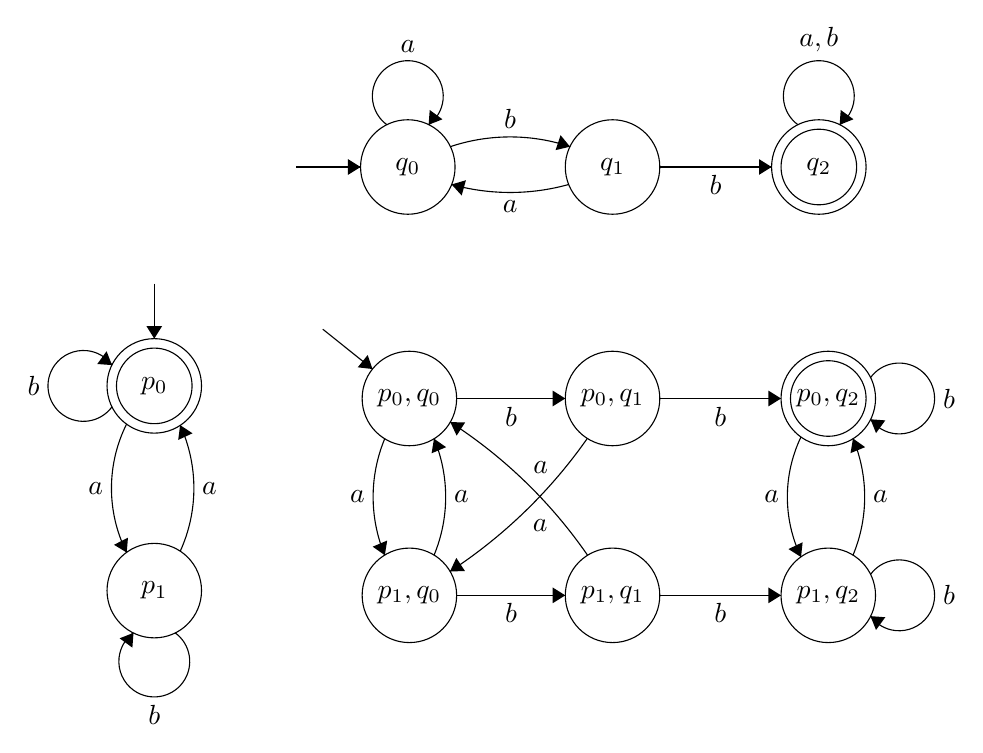
\begin{tikzpicture}[scale=0.2]
\tikzstyle{every node}+=[inner sep=0pt]
\draw [black] (14.8,-25.3) circle (3);
\draw (14.8,-25.3) node {$p_0$};
\draw [black] (14.8,-25.3) circle (2.4);
\draw [black] (14.8,-38.3) circle (3);
\draw (14.8,-38.3) node {$p_1$};
\draw [black] (30.9,-11.4) circle (3);
\draw (30.9,-11.4) node {$q_0$};
\draw [black] (43.9,-11.4) circle (3);
\draw (43.9,-11.4) node {$q_1$};
\draw [black] (57,-11.4) circle (3);
\draw (57,-11.4) node {$q_2$};
\draw [black] (57,-11.4) circle (2.4);
\draw [black] (31,-26.1) circle (3);
\draw (31,-26.1) node {$p_0,q_0$};
\draw [black] (43.9,-26.1) circle (3);
\draw (43.9,-26.1) node {$p_0,q_1$};
\draw [black] (57.6,-26.1) circle (3);
\draw (57.6,-26.1) node {$p_0,q_2$};
\draw [black] (57.6,-26.1) circle (2.4);
\draw [black] (31,-38.6) circle (3);
\draw (31,-38.6) node {$p_1,q_0$};
\draw [black] (43.9,-38.6) circle (3);
\draw (43.9,-38.6) node {$p_1,q_1$};
\draw [black] (57.6,-38.6) circle (3);
\draw (57.6,-38.6) node {$p_1,q_2$};
\draw [black] (14.8,-18.8) -- (14.8,-22.3);
\fill [black] (14.8,-22.3) -- (15.3,-21.5) -- (14.3,-21.5);
\draw [black] (12.12,-26.623) arc (324:36:2.25);
\draw (7.55,-25.3) node [left] {$b$};
\fill [black] (12.12,-23.98) -- (11.77,-23.1) -- (11.18,-23.91);
\draw [black] (16.123,-40.98) arc (54:-234:2.25);
\draw (14.8,-45.55) node [below] {$b$};
\fill [black] (13.48,-40.98) -- (12.6,-41.33) -- (13.41,-41.92);
\draw [black] (13.045,-35.883) arc (-153.42749:-206.57251:9.129);
\fill [black] (13.05,-35.88) -- (13.13,-34.94) -- (12.24,-35.39);
\draw (11.58,-31.8) node [left] {$a$};
\draw [black] (16.445,-27.794) arc (24.5046:-24.5046:9.658);
\fill [black] (16.44,-27.79) -- (16.32,-28.73) -- (17.23,-28.31);
\draw (17.81,-31.8) node [right] {$a$};
\draw [black] (23.8,-11.4) -- (27.9,-11.4);
\fill [black] (27.9,-11.4) -- (27.1,-10.9) -- (27.1,-11.9);
\draw [black] (29.577,-8.72) arc (234:-54:2.25);
\draw (30.9,-4.15) node [above] {$a$};
\fill [black] (32.22,-8.72) -- (33.1,-8.37) -- (32.29,-7.78);
\draw [black] (33.598,-10.107) arc (108.4487:71.5513:12.013);
\fill [black] (41.2,-10.11) -- (40.6,-9.38) -- (40.28,-10.33);
\draw (37.4,-8.99) node [above] {$b$};
\draw [black] (41.119,-12.51) arc (-74.44385:-105.55615:13.868);
\fill [black] (33.68,-12.51) -- (34.32,-13.21) -- (34.59,-12.24);
\draw (37.4,-13.52) node [below] {$a$};
\draw [black] (46.9,-11.4) -- (54,-11.4);
\fill [black] (54,-11.4) -- (53.2,-10.9) -- (53.2,-11.9);
\draw (50.45,-11.9) node [below] {$b$};
\draw [black] (55.677,-8.72) arc (234:-54:2.25);
\draw (57,-4.15) node [above] {$a,b$};
\fill [black] (58.32,-8.72) -- (59.2,-8.37) -- (58.39,-7.78);
\draw [black] (25.5,-21.7) -- (28.66,-24.23);
\fill [black] (28.66,-24.23) -- (28.35,-23.34) -- (27.72,-24.12);
\draw [black] (29.437,-36.053) arc (-157.38674:-202.61326:9.632);
\fill [black] (29.44,-36.05) -- (29.59,-35.12) -- (28.67,-35.51);
\draw (28.2,-32.35) node [left] {$a$};
\draw [black] (32.563,-28.647) arc (22.61326:-22.61326:9.632);
\fill [black] (32.56,-28.65) -- (32.41,-29.58) -- (33.33,-29.19);
\draw (33.8,-32.35) node [right] {$a$};
\draw [black] (34,-26.1) -- (40.9,-26.1);
\fill [black] (40.9,-26.1) -- (40.1,-25.6) -- (40.1,-26.6);
\draw (37.45,-26.6) node [below] {$b$};
\draw [black] (46.9,-26.1) -- (54.6,-26.1);
\fill [black] (54.6,-26.1) -- (53.8,-25.6) -- (53.8,-26.6);
\draw (50.75,-26.6) node [below] {$b$};
\draw [black] (34,-38.6) -- (40.9,-38.6);
\fill [black] (40.9,-38.6) -- (40.1,-38.1) -- (40.1,-39.1);
\draw (37.45,-39.1) node [below] {$b$};
\draw [black] (46.9,-38.6) -- (54.6,-38.6);
\fill [black] (54.6,-38.6) -- (53.8,-38.1) -- (53.8,-39.1);
\draw (50.75,-39.1) node [below] {$b$};
\draw [black] (55.87,-36.167) arc (-154.32992:-205.67008:8.812);
\fill [black] (55.87,-36.17) -- (55.97,-35.23) -- (55.07,-35.66);
\draw (54.5,-32.35) node [left] {$a$};
\draw [black] (59.167,-28.644) arc (22.68806:-22.68806:9.608);
\fill [black] (59.17,-28.64) -- (59.01,-29.57) -- (59.94,-29.19);
\draw (60.41,-32.35) node [right] {$a$};
\draw [black] (42.297,-28.635) arc (-34.99313:-56.81131:32.055);
\fill [black] (33.58,-37.08) -- (34.53,-37.06) -- (33.98,-36.22);
\draw (39.31,-33.75) node [below] {$a$};
\draw [black] (33.595,-27.603) arc (57.16041:34.64404:31.101);
\fill [black] (33.6,-27.6) -- (34,-28.46) -- (34.54,-27.62);
\draw (39.34,-30.92) node [above] {$a$};
\draw [black] (60.28,-37.277) arc (144:-144:2.25);
\draw (64.85,-38.6) node [right] {$b$};
\fill [black] (60.28,-39.92) -- (60.63,-40.8) -- (61.22,-39.99);
\draw [black] (60.28,-24.777) arc (144:-144:2.25);
\draw (64.85,-26.1) node [right] {$b$};
\fill [black] (60.28,-27.42) -- (60.63,-28.3) -- (61.22,-27.49);
\end{tikzpicture}
\end{center}

\begin{bemerkung}
Mit $F_C = \{(p, q) \in Q_C | p \in F_A $ oder $ q \in F_B \}$ funktionert auch für die Vereinigung.
\end{bemerkung}

\item[Mengendifferenz]

Wenn $L$ und $M$ regulär sind, ist auch $L-M$ regulär.

\begin{proof}[Beweis]
Es gilt $L - M = L \cap \overline{M}$. Das Komplement ist regulär, der Schnitt ist regulär, ergo ist $L \cap \overline{M}$ regulär.
\end{proof}

\item[Spiegelung]
\begin{definition}
Sei $w = a_1\dots a_k$ ein Wort. Dann ist $w^\textrm{R} = a_k\dots a_1$ die Spiegelung von $w$.

Sei $L \subseteq \Sigma^*$ eine Sprache. Dann ist $L^\textrm{R} = \{ w \in \Sigma^* | w^\textrm{R} \in L \}$ die Spiegelung von $L$.
 
\end{definition}
\begin{bemerkung} Einige coole Sachen:
\begin{itemize}
\item $\varepsilon^\textrm{R} = \varepsilon$
\item $(w^\textrm{R})^\textrm{R} = w$
\item Wenn $L$ regulär ist, dann ist auch $L^\textrm{R}$ regulär.
\end{itemize}
\end{bemerkung}

\begin{proof}[Beweis]
Sei $A = (Q, \Sigma, \delta, q_0, F)$ ein DEA für $L$. Wir konstruieren einen \enea $B$ für $L^\textrm{R}$ wie folgt:

$B = (Q \cup \{q_S\}, \Sigma, \delta_B, q_S, F_B)$ mit
\begin{enumerate}
\item $F_B = \{q_0 \}$
\item $\delta_B(q, a) = \{p\}$ für $\delta(p,a) = q$
\item $\delta_B(q_S, \varepsilon) = \{p \}$ für alle $p \in F$
\end{enumerate}

$B$ simuliert $A$ in umgekehrter Richtung $\Rightarrow B$ akzeptiert $L^\textrm{R}$.
\end{proof}

\begin{beispiel}
$L = \{w \in \{a,b\}^* | w $ endet auf $ba$ oder $ab\}$.

\begin{center}
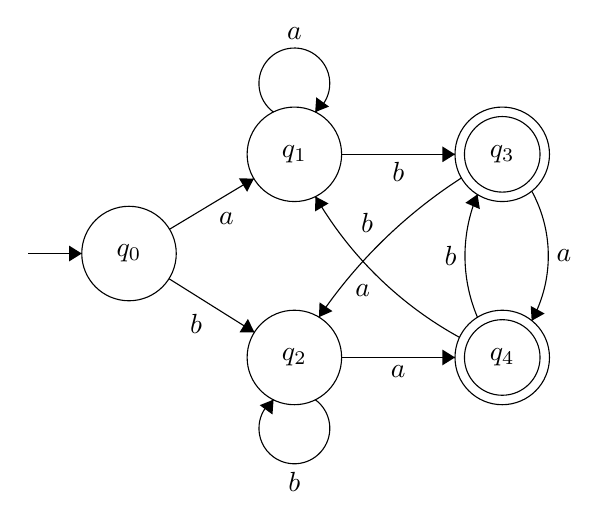
\begin{tikzpicture}[scale=0.2]
\tikzstyle{every node}+=[inner sep=0pt]
\draw [black] (14,-27.2) circle (3);
\draw (14,-27.2) node {$q_0$};
\draw [black] (24.5,-20.9) circle (3);
\draw (24.5,-20.9) node {$q_1$};
\draw [black] (24.5,-33.8) circle (3);
\draw (24.5,-33.8) node {$q_2$};
\draw [black] (37.7,-20.9) circle (3);
\draw (37.7,-20.9) node {$q_3$};
\draw [black] (37.7,-20.9) circle (2.4);
\draw [black] (37.7,-33.8) circle (3);
\draw (37.7,-33.8) node {$q_4$};
\draw [black] (37.7,-33.8) circle (2.4);
\draw [black] (7.6,-27.2) -- (11,-27.2);
\fill [black] (11,-27.2) -- (10.2,-26.7) -- (10.2,-27.7);
\draw [black] (16.57,-25.66) -- (21.93,-22.44);
\fill [black] (21.93,-22.44) -- (20.98,-22.43) -- (21.5,-23.28);
\draw (20.19,-24.55) node [below] {$a$};
\draw [black] (16.54,-28.8) -- (21.96,-32.2);
\fill [black] (21.96,-32.2) -- (21.55,-31.35) -- (21.02,-32.2);
\draw (18.25,-31) node [below] {$b$};
\draw [black] (27.5,-20.9) -- (34.7,-20.9);
\fill [black] (34.7,-20.9) -- (33.9,-20.4) -- (33.9,-21.4);
\draw (31.1,-21.4) node [below] {$b$};
\draw [black] (27.5,-33.8) -- (34.7,-33.8);
\fill [black] (34.7,-33.8) -- (33.9,-33.3) -- (33.9,-34.3);
\draw (31.1,-34.3) node [below] {$a$};
\draw [black] (23.177,-18.22) arc (234:-54:2.25);
\draw (24.5,-13.65) node [above] {$a$};
\fill [black] (25.82,-18.22) -- (26.7,-17.87) -- (25.89,-17.28);
\draw [black] (25.823,-36.48) arc (54:-234:2.25);
\draw (24.5,-41.05) node [below] {$b$};
\fill [black] (23.18,-36.48) -- (22.3,-36.83) -- (23.11,-37.42);
\draw [black] (39.569,-23.227) arc (28.73671:-28.73671:8.575);
\fill [black] (39.57,-31.47) -- (40.39,-31.01) -- (39.51,-30.53);
\draw (41.12,-27.35) node [right] {$a$};
\draw [black] (36.13,-31.257) arc (-156.93869:-203.06131:9.973);
\fill [black] (36.13,-23.44) -- (35.36,-23.98) -- (36.28,-24.38);
\draw (34.83,-27.35) node [left] {$b$};
\draw [black] (26.062,-31.24) arc (145.88482:122.7981:31.592);
\fill [black] (26.06,-31.24) -- (26.92,-30.86) -- (26.1,-30.3);
\draw (29.12,-25.88) node [above] {$b$};
\draw [black] (34.987,-32.524) arc (-118.78623:-149.89669:23.852);
\fill [black] (25.84,-23.58) -- (25.81,-24.53) -- (26.67,-24.02);
\draw (28.84,-29.16) node [below] {$a$};
\end{tikzpicture}
\end{center}

$L^\textrm{R} = \{w \in \{a,b\}^* | w $ beginnt mit $ba$ oder $ab\}$.

\begin{center}
\begin{tikzpicture}[scale=0.2]
\tikzstyle{every node}+=[inner sep=0pt]
\draw [black] (14,-27.2) circle (3);
\draw (14,-27.2) node {$q_0$};
\draw [black] (14,-27.2) circle (2.4);
\draw [black] (24.5,-20.9) circle (3);
\draw (24.5,-20.9) node {$q_1$};
\draw [black] (24.5,-33.8) circle (3);
\draw (24.5,-33.8) node {$q_2$};
\draw [black] (37.7,-20.9) circle (3);
\draw (37.7,-20.9) node {$q_3$};
\draw [black] (37.7,-33.8) circle (3);
\draw (37.7,-33.8) node {$q_4$};
\draw [black] (50.2,-27.2) circle (3);
\draw (50.2,-27.2) node {$q_S$};
\draw [black] (23.177,-18.22) arc (234:-54:2.25);
\draw (24.5,-13.65) node [above] {$a$};
\fill [black] (25.82,-18.22) -- (26.7,-17.87) -- (25.89,-17.28);
\draw [black] (25.823,-36.48) arc (54:-234:2.25);
\draw (24.5,-41.05) node [below] {$b$};
\fill [black] (23.18,-36.48) -- (22.3,-36.83) -- (23.11,-37.42);
\draw [black] (57.7,-27.2) -- (53.2,-27.2);
\fill [black] (53.2,-27.2) -- (54,-27.7) -- (54,-26.7);
\draw [black] (47.52,-25.85) -- (40.38,-22.25);
\fill [black] (40.38,-22.25) -- (40.87,-23.06) -- (41.32,-22.16);
\draw (44.86,-23.55) node [above] {$\epsilon$};
\draw [black] (47.55,-28.6) -- (40.35,-32.4);
\fill [black] (40.35,-32.4) -- (41.29,-32.47) -- (40.83,-31.58);
\draw (43.03,-30) node [above] {$\epsilon$};
\draw [black] (34.7,-33.8) -- (27.5,-33.8);
\fill [black] (27.5,-33.8) -- (28.3,-34.3) -- (28.3,-33.3);
\draw (31.1,-33.3) node [above] {$a$};
\draw [black] (34.7,-20.9) -- (27.5,-20.9);
\fill [black] (27.5,-20.9) -- (28.3,-21.4) -- (28.3,-20.4);
\draw (31.1,-20.4) node [above] {$b$};
\draw [black] (21.93,-22.44) -- (16.57,-25.66);
\fill [black] (16.57,-25.66) -- (17.52,-25.67) -- (17,-24.82);
\draw (18.31,-23.55) node [above] {$a$};
\draw [black] (21.96,-32.2) -- (16.54,-28.8);
\fill [black] (16.54,-28.8) -- (16.95,-29.65) -- (17.48,-28.8);
\draw (20.25,-30) node [above] {$b$};
\draw [black] (25.372,-30.934) arc (157.87246:110.81046:16.534);
\fill [black] (34.81,-21.71) -- (33.89,-21.52) -- (34.24,-22.46);
\draw (28.11,-24.86) node [above] {$b$};
\draw [black] (34.921,-32.678) arc (-116.14106:-152.54185:20.671);
\fill [black] (34.92,-32.68) -- (34.42,-31.88) -- (33.98,-32.77);
\draw (28.62,-29.38) node [below] {$a$};
\draw [black] (36.168,-31.233) arc (-157.60898:-202.39102:10.194);
\fill [black] (36.17,-31.23) -- (36.33,-30.3) -- (35.4,-30.68);
\draw (34.9,-27.35) node [left] {$b$};
\draw [black] (39.104,-23.541) arc (20.20784:-20.20784:11.028);
\fill [black] (39.1,-23.54) -- (38.91,-24.46) -- (39.85,-24.12);
\draw (40.28,-27.35) node [right] {$a$};
\end{tikzpicture}
\end{center}

\end{beispiel}

\begin{proof}[Beweis über Reguläre Ausdrücke]

Sei $\alpha$ ein regulärer Ausdruck mit $L(\alpha) = L$.

Zu zeigen: Es gibt einen RA $\beta$ mit $L(\beta) = (L(\alpha))^\textrm{R} = L^\textrm{R}$.

Strukturelle Induktion über den Aufbau von $\alpha$. Induktionsanfang:

\begin{itemize}
\item $\varepsilon^\textrm{R} = \varepsilon$
\item $\varnothing^\textrm{R} = \varnothing$
\item $a^\textrm{R} = a$ für ein $a \in \Sigma$
\end{itemize}

Induktionsschritt:
\begin{itemize}
\item Vereinigung $\alpha = \alpha_1 + \alpha_2$:
\[
L(\alpha_1 + \alpha_2)^\textrm{R} = (L(\alpha_1) \cup L(\alpha_2))^\textrm{R} = L(\alpha_1)^\textrm{R} \cup L(\alpha_2)^\textrm{R} \Rightarrow \alpha^\textrm{R} = \alpha_1^\textrm{R} + \alpha_2^\textrm{R}
\]
\item Konkatenation $\alpha = \alpha_1 \alpha_2$:
\[
L(\alpha_1 \alpha_2)^\textrm{R} =  (L(\alpha_1) L(\alpha_2))^\textrm{R} = L(\alpha_1)^\textrm{R} L(\alpha_2)^\textrm{R} \Rightarrow \alpha^\textrm{R} \overset{(w_1 w_2)^\textrm{R} = w_2^\textrm{R} w_1^\textrm{R}}{=} \alpha_1^\textrm{R} \alpha_2^\textrm{R}
\]
\item Kleene'scher Stern $\alpha = \alpha_1^*$:
\[
L(\alpha_1^*)^\textrm{R} = (L(\alpha_1)^\textrm{R})^* \rightarrow \alpha^\textrm{R} = (\alpha_1^\textrm{R})^*
\]
\end{itemize}

\end{proof}

\item[Homomorphismus]

\begin{definition} Ein (Wort-)Homomorphismus ist eine Abbildung
\[
h : \Sigma_1 \mapsto \Sigma_2^*
\]

die die Symbole eines Alphabets auf Wörter abbildet.
\end{definition}

\begin{beispiel}
$\Sigma_1 = \{0,1 \}, \Sigma_2 = \{a,b\}, h(0) = ab, h(1) = \varepsilon$
\end{beispiel}

Erweiterung auf Wörter: Sei $w = a_1\dots a_k$. Dann ist $h(w) = h(a_1)\cdot h(a_2)\cdot \dots \cdot h(a_k)$.

\begin{beispiel}
$h(0101) = ab\cdot \varepsilon \cdot ab \cdot \varepsilon = abab$
\end{beispiel}

\begin{definition}
Sei $h : \Sigma_1 \mapsto \Sigma_2^*$ ein Homomorphismus, sei $L \subseteq \Sigma_1^*$ eine Sprache. Dann ist
\[
h(L) = \{ w \in \Sigma^* | w = h(x) \textrm{ für ein } x \in L \}
\]
\end{definition}

Satz: Sei $h : \Sigma_1 \mapsto \Sigma_2^*$ ein Homomorphismus. Wenn $L \subseteq L_1^*$ regulär ist, dann ist auch $h(L)$ regulär.

\begin{proof}[Beweis über rock-the-bottom strukturelle Induktion]
Für einen regulären Ausdruck $\alpha$ über $\Sigma_1$ ist $h(\alpha)$ der reguläre Ausdruck über $\Sigma_2$, der entsteht, wenn jedes Vorkommen von $a \in \Sigma_1$ durch $h(a)$ ersetzt wird. 
\end{proof}

\begin{beispiel}
$\Sigma_1 = \{0,1\}, \Sigma_2 = \{a,b\}, h(0) = ab, h(1) = \varepsilon$.
\[
\alpha = ((0+1)0)^* 1 \Rightarrow h(\alpha) ((ab + \varepsilon)\cdot ab)^*\varepsilon = (ab)^*
\]
\end{beispiel}

Und latürnich gilt: $L(h(\alpha)) = h(L)$

\begin{beispiel}[Übungsaufgaben 9. Oktober -- Aufgabe 3]
Deifniere die Menge der $a$-Vorgänger eines Zustands $q$ als $V_a(q) = \{ p \in Q | \delta(p, a) = q \}$. Dann ist $B = (Q, \Sigma, \delta, q_0, V_a(F))$ ein DEA für $L/a$.
\end{beispiel}

\end{description}

\subsection{Nichtregularität}

Ziel: Zeige, dass es Sprachen gibt, die nicht regulär sind.

Idee: DEAs analysieren: DEAs können nicht beliebig weit zählen.

\begin{beispiel}
Betrachte den folgenden DEA:

\begin{center}
\begin{tikzpicture}[scale=0.2]
\tikzstyle{every node}+=[inner sep=0pt]
\draw [black] (13.6,-17.3) circle (3);
\draw (13.6,-17.3) node {$q_0$};
\draw [black] (26.5,-17.3) circle (3);
\draw (26.5,-17.3) node {$q_1$};
\draw [black] (40.4,-17.3) circle (3);
\draw (40.4,-17.3) node {$q_4$};
\draw [black] (40.4,-17.3) circle (2.4);
\draw [black] (40.3,-30.3) circle (3);
\draw (40.3,-30.3) node {$q_2$};
\draw [black] (26.5,-30.3) circle (3);
\draw (26.5,-30.3) node {$q_3$};
\draw [black] (12.277,-14.62) arc (234:-54:2.25);
\draw (13.6,-10.05) node [above] {$a$};
\fill [black] (14.92,-14.62) -- (15.8,-14.27) -- (14.99,-13.68);
\draw [black] (16.6,-17.3) -- (23.5,-17.3);
\fill [black] (23.5,-17.3) -- (22.7,-16.8) -- (22.7,-17.8);
\draw (20.05,-17.8) node [below] {$b$};
\draw [black] (29.5,-17.3) -- (37.4,-17.3);
\fill [black] (37.4,-17.3) -- (36.6,-16.8) -- (36.6,-17.8);
\draw (33.45,-17.8) node [below] {$b$};
\draw [black] (28.68,-19.36) -- (38.12,-28.24);
\fill [black] (38.12,-28.24) -- (37.88,-27.33) -- (37.19,-28.06);
\draw (32.44,-24.28) node [below] {$a$};
\draw [black] (27.823,-32.98) arc (54:-234:2.25);
\draw (26.5,-37.55) node [below] {$b$};
\fill [black] (25.18,-32.98) -- (24.3,-33.33) -- (25.11,-33.92);
\draw [black] (37.3,-30.3) -- (29.5,-30.3);
\fill [black] (29.5,-30.3) -- (30.3,-30.8) -- (30.3,-29.8);
\draw (33.4,-29.8) node [above] {$a$};
\draw [black] (42.98,-28.977) arc (144:-144:2.25);
\draw (47.55,-30.3) node [right] {$b$};
\fill [black] (42.98,-31.62) -- (43.33,-32.5) -- (43.92,-31.69);
\draw [black] (43.08,-15.977) arc (144:-144:2.25);
\draw (47.65,-17.3) node [right] {$a,b$};
\fill [black] (43.08,-18.62) -- (43.43,-19.5) -- (44.02,-18.69);
\draw [black] (26.5,-27.3) -- (26.5,-20.3);
\fill [black] (26.5,-20.3) -- (26,-21.1) -- (27,-21.1);
\draw (27,-23.8) node [right] {$a$};
\draw [black] (8.8,-17.3) -- (10.6,-17.3);
\fill [black] (10.6,-17.3) -- (9.8,-16.8) -- (9.8,-17.8);
\end{tikzpicture}
\end{center}

Arbeit von $A$ auf dem Wort $w=abaaab$:
\[
q_0
\overset{a}{\mapsto} q_0
\overset{b}{\mapsto} q_1
\overset{a}{\mapsto} q_2
\overset{a}{\mapsto} q_3
\overset{a}{\mapsto} q_1
\overset{b}{\mapsto} q_4
\]

Enthält einen Zykel $q_1 \overset{a}{\mapsto}q_2 \overset{a}{\mapsto}q_3 \overset{a}{\mapsto}q_1$.

Wiederholung des Zykels: $w' = ab aaa aaa b$

\[
q_0
\overset{a}{\mapsto} q_0
\overset{b}{\mapsto} q_1
\overset{a}{\mapsto} q_2
\overset{a}{\mapsto} q_3
\overset{a}{\mapsto} q_1
\overset{a}{\mapsto} q_2
\overset{a}{\mapsto} q_3
\overset{a}{\mapsto} q_1
\overset{b}{\mapsto} q_4
\]

Da $q_4 \in F$, gilt $w' \in L(A)$

\end{beispiel}

Allgemein: Sei $A$ ein DEA. Sei $w = u\cdot x \cdot v$ ein Wort in $L(A)$, $u,v,x \in \Sigma^*, x \neq \varepsilon$. Falls der Automat auf dem Teilwort $x$ in einer Schleife läuft, dann ist auch das Wort $w' = uxxv \in L(A)$.

Formal: Falls $\hat\delta(q_0, u) = q$ und $\hat\delta(q, x) = q$ und $\hat\delta(q, v) \in F$, dann ist $w' = uxxv \in L(A)$.

Im Beispiel oben:
\[
w = \underbrace{u}_{ab}\underbrace{x}_{aaa}\underbrace{v}_{b} \in L(A)
\]
, $w' = \underbrace{u}_{ab}\underbrace{x}_{aaa}\underbrace{x}_{aaa}\underbrace{v}_{b} \in L(A)$

\begin{bemerkung}
Ein DEA ist vollständig, d.h. für jedes $q \in Q$ und jedes $a \in \Sigma$ existiert genau ein Folgezustand $\delta(q, a)$. Daraus folgt direkt, dass man mit jedem Wort aus $\Sigma^*$ kann man durch den Automaten laufen, ohne stecken zu bleiben. Daraus wiederum folgt, dass bei der Arbeit des DEA $A$ mit $n$ Zuständen auf einem Wort der Länge $\ge n$ wird mindestens ein Zustand doppelt besucht.
\end{bemerkung}

\begin{beispiel} Sei
\begin{center}
\begin{tikzpicture}[scale=0.2]
\tikzstyle{every node}+=[inner sep=0pt]
\draw [black] (13.6,-17.3) circle (3);
\draw (13.6,-17.3) node {$q_0$};
\draw [black] (26.5,-17.3) circle (3);
\draw (26.5,-17.3) node {$q_1$};
\draw [black] (40.4,-17.3) circle (3);
\draw (40.4,-17.3) node {$q_2$};
\draw [black] (40.4,-17.3) circle (2.4);
\draw [black] (16.202,-15.826) arc (111.38395:68.61605:10.555);
\fill [black] (23.9,-15.83) -- (23.34,-15.07) -- (22.97,-16);
\draw (20.05,-14.6) node [above] {$a$};
\draw [black] (29.139,-15.89) arc (110.97997:69.02003:12.04);
\fill [black] (37.76,-15.89) -- (37.19,-15.14) -- (36.83,-16.07);
\draw (33.45,-14.59) node [above] {$a$};
\draw [black] (43.08,-15.977) arc (144:-144:2.25);
\draw (47.65,-17.3) node [right] {$a$};
\fill [black] (43.08,-18.62) -- (43.43,-19.5) -- (44.02,-18.69);
\draw [black] (8.8,-17.3) -- (10.6,-17.3);
\fill [black] (10.6,-17.3) -- (9.8,-16.8) -- (9.8,-17.8);
\draw [black] (23.773,-18.532) arc (-72.58873:-107.41127:12.441);
\fill [black] (16.33,-18.53) -- (16.94,-19.25) -- (17.24,-18.29);
\draw (20.05,-19.6) node [below] {$b$};
\draw [black] (37.582,-18.318) arc (-75.38527:-104.61473:16.378);
\fill [black] (29.32,-18.32) -- (29.97,-19) -- (30.22,-18.04);
\draw (33.45,-19.35) node [below] {$b$};
\draw [black] (15.286,-14.824) arc (140.11895:39.88105:15.265);
\fill [black] (38.71,-14.82) -- (38.58,-13.89) -- (37.82,-14.53);
\draw (27,-8.85) node [above] {$b$};
\end{tikzpicture}
\end{center}

$|Q| = 3$.

z.B. $w_1 = abb$: $q_0 \overset{a}{\mapsto} q_1 \overset{b}{\mapsto} q_0 \overset{b}{\mapsto} q_2$

$\Rightarrow$ $q_0$ doppelt besucht.
\end{beispiel}

Beobachtung: Sei $A = (Q, \Sigma, \delta, q_0, F)$ ein DEA mit $|Q| = n$. Sei $w \in L(A)$ mit $|w| \ge n$. Dann wiederholt sich in der Berechnung von $A$ auf $w$ mindestens einmal ein Zustand. Wir nennen einen dieser wiederholt besuchten Zustände $q_x$. Dann lässt sich $w$ zerlegen in drei Teile
\[
w = \underbrace{u}_{\textrm{bis zum ersten $q_x$}} \cdot \underbrace{x}_{\textrm{von $q_x$ nach $q_x$}} \cdot \underbrace{v}_{\textrm{nach $q_x$}}
\]

Berechnug von $A$ auf $w$ hat die Form
\[
q_0 \overset{u}{\leadsto} q_x \overset{x}{\leadsto} q_x \overset{v}{\leadsto} q_F \in F
\]

Damit gibt es auch eine Berechnung von $A$ auf $w' = uxxv$:
\[
q_0 \overset{u}{\leadsto} q_x \overset{x}{\leadsto} q_x q_x \overset{x}{\leadsto} q_x \overset{v}{\leadsto} q_F \in F
\]

\begin{beispiel}
Diese Beobachtung können wir nutzen, um zu zeigen, dass $L = \{a^k b^k | k \ge 0 \}$ nicht regulär ist.
\end{beispiel}

\begin{proof}[Beweis durch Widerspruch]
Für $L$ kann es keinen DEA mit 7 Zuständen geben.

Annahme: Es gibt einen DEA $A = (Q, \Sigma, \delta, q_0, F)$ mit $|Q| = 7$ und $\Sigma = \{a,b\}$, so dass $L(A) = L$.

Es gibt zwei Möglichkeiten zur Widerlegung:

\begin{enumerate}
\item alle möglichen DEA mit 7 Zuständen ausprobieren. Klappt nicht, weil zu viele. 
\item Beobachtung über Zykel ausnutzen.

Betrachte das Wort $w = aaaabbbb \in L$. Es gilt $|w| = 8 > 7 = |Q|$. Also muss sich in der Berechnung von $A$ auf $w$ mindestens ein Zustand wiederholen.

Zerteilen wir $w$ in $w = u\cdot x \cdot v$ mit der Berechnung
\[
q_0 \overset{u}{\leadsto}
q_x \overset{x}{\leadsto}
q_x \overset{v}{\leadsto}
q_F \in F
\]

Daraus folgt $w' = uxxv \in L(A)$.
Wie kann das Wort $x$ aussehen? Fallunterscheidung:
\begin{enumerate}
\item $x$ besteht nur aus $a$s. z.B. $w = \underbrace{aa}_u\underbrace{aa}_x \underbrace{bbbb}_v$. Daraus folgt $w' = \underbrace{aa}_u\underbrace{aa}_x \underbrace{aa}_x \underbrace{bbbb}_v = a^6 b^4 \not\in L$. Widerspruch!

\item $x$ besteht nur aus $b$s. z.B. $w = \underbrace{aaaab}_u\underbrace{b}_x \underbrace{bb}_v$. Daraus folgt $w' = \underbrace{aaaab}_u\underbrace{b}_x \underbrace{b}_x \underbrace{bb}_v = a^4 b^5 \not\in L$. Widerspruch!

\item $x$ besteht aus $a$s und $b$s. z.B. $w = \underbrace{aa}_u\underbrace{aab}_x \underbrace{bbb}_v$. Daraus folgt $w' = \underbrace{aa}_u\underbrace{aab}_x \underbrace{aab}_x \underbrace{bbb}_v  \not\in L$. Widerspruch!

Daraus folgt, dass es keinen DEA mit 7 Zuständen für $L$ gibt.

Denselben Beweis hätten wir auch für jede andere Anzahl von Zuständen führen können. Daraus kann gefolgert werden, dass es überhaupt keinen DEA für $L$ gibt. Daraus folgt, dass $L$ nicht regulär ist.
\end{enumerate}

\end{enumerate}
\end{proof}

\begin{beispiel}
Argumentieren wir, warum ein DEA mit 5 Zuständen die Sprache
\[
	L = \{a^kb^{2k} | k \ge 0 \}
\]
nicht akzeptieren kann.
\end{beispiel}

\begin{proof}[Beweis]
Annahme: Es gibt einen DEA mit $|Q|=5$. Betrachten wir uns das Wort $w = aabbbb \in L$. Es gilt $|w|$ = 6, das heisst es wird mindestens 1 Zustand mehrfach durchlaufen. $w$ lässt sich also zerlegen in $w = uxv$:
\[
q_0 \overset{u}{\leadsto} q_x \overset{x}{\leadsto} q_F \in F.
\]
Dann gilt $w' = uxxv \in L(A)$.

Fallunterscheidung über die Form von $x$:
\begin{enumerate}
\item $x$ besteht nur aus $a$s. D.h. $w'$ enthält mehr $a$s als $w$, aber nicht mehr $b$s $ \Rightarrow w' \notin L$. Widerspruch!
\item $x$ besteht nur aus $b$s. Analoger Widerspruch.
\item $x$ besteht aus $a$s und $b$s. $\Rightarrow $ in $w'$ kommt ein $b$ vor einem $a \Rightarrow w' \notin L$. Darum gibt es keinen DEA mit 5 Zuständen, der $L$ akzeptieren könnte.
\end{enumerate}
\end{proof}

\subsection{Verallgemeinerung der Methode}

Ziel: Zeige, dass es gar keinen DEA für $L$ gibt.

\begin{definition}[Pumping-Lemma für reguläre Sprachen]

Sei $L$ eine reguläre Sprache. Dann gibt es eine Konstante $n_0$ (die von $L$ abhängt), so dass für jedes Wort $w \in L$ mit $|w| \ge n_0$ gilt:

$w$ kann zerlegt werden in $w = uxv$ mit den folgenden Eigenschaften:
\begin{enumerate}[(a)]
\item $|w| \ge 1$, d.h. $x \neq \varepsilon$
\item $|ux| \le n_0$
\item Für alle $k \ge 0$ ist auch $ux^kv \in L$.
\end{enumerate}

\end{definition}

\begin{proof}[Begründung der Korrektheit]
Falls $L$ regulär ist, existiert ein DEA $A$ für $L$. Setzen wir $n_0 = |Q|$. $x$ ist dann die Beschriftung eines Zykels in $A$, der in den ersten $|Q|$ Berechnungsschritten auftritt ($|ux| \le n_0$). Eine Wiederholung des Zykels ändert nichts an der Akzeptanz des Wortes.
\end{proof}

\begin{beispiel}
Zeigen wir, dass $L = \{a^kb^k | k \in \mathbb{N} \}$.
\end{beispiel}
\begin{proof}[Beweis]
Annahme: $L$ ist regulär. Das Pumping-Lemma gibt uns die Existenz einer Konstanten $n_0$, sodass für alle Wörter $w \in L$ mit $|w| \ge n_0$ alle Bedingungen gelten.
Um einen Widerspruch herzuleiten, können wir uns ein Wort $w \in L$ auswählen, sei also $w = a^{n_0}b^{n_0}$. Nach dem Pumping-Lemma gibt es eine Zerlegung $w = uxv$ mit $|ux| \le n_0$ und $|x| \ge 1$.

Daraus folgt, dass:
\[
u = a^j \textrm{ für ein } 0 \le j \le n_0 \le n_0
\]
und
\[
x = a^i \textrm{ für ein } 1 \le i \le n_0.
\]
Weiter gilt nach dem Pumping-Lemma: $ux^kv \in L$ für alle $k$.
Um den Widerspruch herzuleiten, wählen wir $k = 2$. Nach dem Pumping-Lemma muss gelten, dass
\[
ux^2v = a^{n_0 + i}b^{n_0} \in L.
\]
Das ist ein Widerspruch weil $n_0 + i \neq n_0$. Also kann $L$ nicht regulär sein.
\end{proof}

\begin{bemerkung}
So nützlich es auch ist, aber:
\begin{itemize}
\item Das Pumping-Lemma gibt nur notwendige Eigenschaften für reguläre Sprachen an, aber keine hinreichenden. Die Regularität einer Sprache kann also damit nicht gezeigt werden.
\item Es gibt Sprachen, die nicht regulär sind und trotzdem das Pumping-Lemma erfüllen. Dumm gelaufen.

\end{itemize}
\end{bemerkung}

\subsection{Anwendung des Pumping-Lemmas gegen einen Gegner}

Wir spielen gegen Darth Vader, die Lemmings und die Achse der bösen Allquantoren.
\begin{enumerate}
\item Wir wählen die Sprache, deren Nichtregularität wir nachweisen wollen.
\item Darth Vader wählt $n_0$.
\item Wir wählen das Wort $w$ mit $|w| \ge n_0$.
\item Darth Vader lässt sich davon nicht beeindrucken und zerlegt $w = uxv$ gemäss dem Pumping-Lemma.
\item Wir wählen $k$ und gewinnen, falls wir einen Widerspruch herleiten können.
\end{enumerate}

\begin{beispiel} Viele viele Aufgaben:
\begin{enumerate}[(a)]
\item Nicht regulär: $L = \{0^m10^m\}, m \ge 1$

Annahme: $L$ ist regulär. Darum gibt es $n_0$, sodass alle Pumping-Lemma-Bedingungen gelten. $w = 0^{n_0}10^{n_0}$.

Zerlegung: $w = uxv$. $u = 0^j$, $x = 1$. $ux^kv \in L$ für alle $k$. $k = 2$. Daraus folgt: $ux^2v = 0^{n_0}1^20^{n_0}$. Foul.

\item Nicht regulär: $L = \{yy^\textrm{R} | y \in \{a,b^*\} \}$

Annahme: $L$ ist regulär. Darum gibt es $n_0$, sodass alle Pumping-Lemma-Bedingungen gelten. $w = a^{n_0}bba^{n_0}$. Zerlegung. $\Rightarrow |ux| \le n_0, |x| \ge 1$, also
\[
u = a^j, x = a^i
\]

Gem. Pumping-Lemma ist $ux^0v = uv-a^{n_0-i}bba^{n_0}$. Widerspruch.

\end{enumerate}
\end{beispiel}

\begin{beispiel}
6a. Differenz: Offenbar $0^*1^*$ regulär. Annahme: $L_1$ ist regulär.
\[
\{0^m1^m\} = 0^*1^* - \{0^i1^j | i \neq j \}. 
\]

6b. Homomorphismus: $h: \{ a,b,c\} \mapsto \{0,1\}$. $h(a) = 0, h(b) = 0, h(c) = 1$.

$h(L_2) = \{0^m0^l1^{m+l} | l, m \ge 0\}$
\end{beispiel}

\section{Reguläre Grammatiken}

Idee: Mechanismus zur Erzeugung aller Wörter aus einer Sprache.

\begin{beispiel} Reguläre Sprache:
\[
L = \{1w | w \in 0^* \} \subseteq \{0,1\}^* = \{1, 10, 100, 1000, \dots \}
\]

Vorgehen bei der Konstruktion solcher Wörter:
\begin{itemize}
\item 1 an den Anfang setzen
\item beliebig viele 0 auffüllen.
\end{itemize}

Regeln:
\begin{enumerate}[(1)]
\item start $\rightarrow 1N$
\item $N \rightarrow 0N$
\item $N \rightarrow \varepsilon$
\end{enumerate}

Konstruktion von 1000:

start $\overset{(1)}{\Rightarrow} 1N \overset{(2)}{\Rightarrow} 10N \overset{(2)}{\Rightarrow} 100N \overset{(2)}{\Rightarrow} 1000N \overset{(3)}{\Rightarrow} 1000$

\end{beispiel}

\begin{definition}
Eine Rechtslineare Grammatik $G$ erzeugt alle Wörter einer Sprache buchstabenweise von links nach rechts. Sie wird beschrieben durch
\[
G = (N,T,P,S),
\]
wobei
\begin{itemize}
\item $T$ das Terminalalphabet (Alphabet der Sprache)
\item $N$ das Nichtterminalalphabet (Menge von Hilfssymbolen)
\item $P \subseteq N \times (TN \cup T \cup \{\varepsilon\})$ die Menge von Produktionen (Regeln). Für $p = (l,r)$ heisst $l$ die linke Seite von $P$ und $r$ die rechte Seite von $P$. Wir schreiben statt $p = (l,r)$ auch $l \rightarrow r$
\item $S \in N$ ist das Startsymbol
\end{itemize}
\end{definition}

Anschauung: Produktion $p = l \rightarrow r$ ist eine Ersetzungsregel. In einem Wort über $T\cup N$ wird durch Anwendung von $p$ ein Vorkommen von $l$ durch $r$ ersetzt.

\begin{definition}[Ableitungsschritt]
Sei $G = (N,T,P,S)$ eine rechtslineare Grammatik. Ein Ableitungsschritt in $G$ ist eine Relation
\[
\Rightarrow \subseteq T^*N\times T^* (N\cup \varepsilon)
\]
definiert durch $uA \Rightarrow uw$ genau dann, wenn $A \rightarrow w \in P$, wobei $u \in T^*, A\in N, w \in TN \cup T\cup \{\varepsilon\}$.
\end{definition}

\begin{definition}[Ableitung]
Eine Ableitung ist eine endliche Folge von Ableitungsschritten. Formal ist $\overset{*}{\Rightarrow}$ die reflexive, transitive Hülle von $\Rightarrow$.

Die von $G$ erzeugte Sprache ist definiert als
\[
L(G) =  \{w \in \Sigma^* | S \overset{*}{\Rightarrow} w \},
\]
also die Menge aller Wörter, die aus $S$ in endlich vielen Ableitungsschritten erzeugt werden können.

\end{definition}

\begin{definition}[Äquivalenz von Grammatiken]
Zwei Grammatiken sind $G_1, G_2$ heissen äquivalent, falls
\[
L(G_1) = L(G_2).
\]

\end{definition}

\begin{beispiel}
Ein Beispiel:
\[
G = (\{S,A,B\}, \{0,1\}, P, S),
\]
wobei
\[
P = \{ S \overset{(1)}{\rightarrow} 0S, S \overset{(2)}{\rightarrow} 1S, S \overset{(3)}{\rightarrow} 0A, A \overset{(4)}{\rightarrow} 0B, A \overset{(5)}{\rightarrow} 1B, B \overset{(6)}{\rightarrow} 0, B \overset{(7)}{\rightarrow} 1\}
\]

Ableitung von 011010:

\begin{eqnarray*}
S \overset{(1)}{\Rightarrow} 0S \overset{(2)}{\Rightarrow} 01S \overset{(2)}{\Rightarrow} 011S \overset{(3)}{\Rightarrow} 0110A \overset{(5)}{\Rightarrow} 01101B \overset{(6)}{\Rightarrow}011010
\end{eqnarray*}

Ableitung von 0111:

Zwei Regeln für $S$:

\[
S \overset{(1)}{\Rightarrow} 0S \overset{(2)}{\Rightarrow}01S \overset{(2)}{\Rightarrow} 011S \overset{(2)}{\Rightarrow} 0111S \dots
\]

Klappt nicht.

\[
S \overset{(3)}{\Rightarrow} 0A \overset{(5)}{\Rightarrow}01B \overset{(7)}{\Rightarrow} 011
\]

Klappt ebenfalls nicht.

\end{beispiel}

\begin{definition}
\[
\mathcal{L}_{\textrm{rlin}} = \{ L | \textrm{ es existiert eine rechtslineare Grammatik $G$ mit } L= L(G) \}
\]
\end{definition}

Vereinfachung rechtslinearer Grammatiken. 3 Typen von Regeln:

\begin{enumerate}[(1)]
\item $A \rightarrow aB$
\item $A \rightarrow a$
\item $A \rightarrow \varepsilon$
\end{enumerate}

Zeige: Die Regel (2) kann vermieden werden: Ersetze $A \rightarrow a$ durch $A\rightarrow aC$ und $C \rightarrow \varepsilon$.

Weitere Vereinfachung: Es reicht, eine Regel vom Typ (3), zusätzlich wird gegebenenfalls $S \rightarrow \varepsilon$, falls $\varepsilon \in L(G)$. Wie funktioniert das? Ersetze die Regeln $A_1 \rightarrow a_1B_1, \dots, A_k \rightarrow a_kB_k$ und
$B_1 \rightarrow \varepsilon, \dots, B_k \rightarrow \varepsilon$
durch
$A_1 \rightarrow a_1T, \dots, A_k \rightarrow a_kT$ und $T \rightarrow \varepsilon$.

\begin{theorem}[Äquivalenz von rechtslinearen Grammatiken und Endlichen Automaten]
Zu jeder rechtslinearen Grammatik über $T = \Sigma$ existiert ein NEA $A$ über $\Sigma$ mit $L(A) = L(G)$.
\end{theorem}
\begin{proof}[Beweis]
$G = (N, \Sigma, P, S)$ ohne Typ (2).

Daraus folgt: NEA $A = (Q, \Sigma, \delta, q_0, F)$ mit
\begin{itemize}
\item $Q = N$
\item $q_0 = S$
\item $F = \{X \in N | X \rightarrow \varepsilon \in P \}$
\item $\delta$ definiert durch: $X \in \delta (Y, a) \Leftrightarrow Y \rightarrow aY \in P$
\end{itemize}

\end{proof}

\begin{beispiel}
$G = (\{S,A,B\}, \{a,b\}, P, S)$ mit

$P = \{ S \rightarrow aB, S \rightarrow bA, A \rightarrow aB, B \rightarrow bA, A \rightarrow \varepsilon, B \rightarrow \varepsilon\}$.

NEA für $L(G)$:

\begin{center}
\begin{tikzpicture}[scale=0.2]
\tikzstyle{every node}+=[inner sep=0pt]
\draw [black] (15.5,-27) circle (3);
\draw (15.5,-27) node {$S$};
\draw [black] (32.1,-17.4) circle (3);
\draw (32.1,-17.4) node {$A$};
\draw [black] (32.1,-17.4) circle (2.4);
\draw [black] (32.1,-36.3) circle (3);
\draw (32.1,-36.3) node {$B$};
\draw [black] (32.1,-36.3) circle (2.4);
\draw [black] (7.4,-27) -- (12.5,-27);
\fill [black] (12.5,-27) -- (11.7,-26.5) -- (11.7,-27.5);
\draw [black] (18.1,-25.5) -- (29.5,-18.9);
\fill [black] (29.5,-18.9) -- (28.56,-18.87) -- (29.06,-19.74);
\draw (24.8,-22.7) node [below] {$b$};
\draw [black] (30.91,-33.549) arc (-160.81873:-199.18127:20.39);
\fill [black] (30.91,-33.55) -- (31.12,-32.63) -- (30.17,-32.96);
\draw (29.28,-26.85) node [left] {$a$};
\draw [black] (33.484,-20.057) arc (22.64444:-22.64444:17.642);
\fill [black] (33.48,-20.06) -- (33.33,-20.99) -- (34.25,-20.6);
\draw (35.34,-26.85) node [right] {$b$};
\draw [black] (18.12,-28.47) -- (29.48,-34.83);
\fill [black] (29.48,-34.83) -- (29.03,-34.01) -- (28.54,-34.88);
\draw (22.86,-32.15) node [below] {$a$};
\end{tikzpicture}
\end{center}

\end{beispiel}

\begin{theorem}
Zu jedem DEA $A$ über $\Sigma$ existiert eine rechtslineare Grammatik $G$ über $\Sigma = T$ mit $L(G) = L(A)$.
\end{theorem}

\begin{proof}
$A = (Q, \Sigma, \delta,  q_0, F)$

$\Rightarrow G = (N, \Sigma, P, S)$ mit
\begin{itemize}
\item $N = G$
\item $S = q_0$
\item $P$ definiert durch $p \rightarrow aq \in P \Leftrightarrow \delta(p, a) = q$ und $q \rightarrow \varepsilon \in P \Leftrightarrow q \in F$.
\end{itemize}
\end{proof}

\begin{beispiel}
\begin{center}
\begin{tikzpicture}[scale=0.2]
\tikzstyle{every node}+=[inner sep=0pt]
\draw [black] (9.6,-18.6) circle (3);
\draw (9.6,-18.6) node {$q_0$};
\draw [black] (24.4,-18.6) circle (3);
\draw (24.4,-18.6) node {$q_1$};
\draw [black] (39.6,-18.6) circle (3);
\draw (39.6,-18.6) node {$q_2$};
\draw [black] (54.9,-18.6) circle (3);
\draw (54.9,-18.6) node {$q_3$};
\draw [black] (54.9,-18.6) circle (2.4);
\draw [black] (3.3,-18.6) -- (6.6,-18.6);
\fill [black] (6.6,-18.6) -- (5.8,-18.1) -- (5.8,-19.1);
\draw [black] (8.277,-15.92) arc (234:-54:2.25);
\draw (9.6,-11.35) node [above] {$b$};
\fill [black] (10.92,-15.92) -- (11.8,-15.57) -- (10.99,-14.98);
\draw [black] (12.6,-18.6) -- (21.4,-18.6);
\fill [black] (21.4,-18.6) -- (20.6,-18.1) -- (20.6,-19.1);
\draw (17,-19.1) node [below] {$a$};
\draw [black] (27.4,-18.6) -- (36.6,-18.6);
\fill [black] (36.6,-18.6) -- (35.8,-18.1) -- (35.8,-19.1);
\draw (32,-19.1) node [below] {$b$};
\draw [black] (42.6,-18.6) -- (51.9,-18.6);
\fill [black] (51.9,-18.6) -- (51.1,-18.1) -- (51.1,-19.1);
\draw (47.25,-19.1) node [below] {$a$};
\draw [black] (57.746,-17.69) arc (135.46923:-152.53077:2.25);
\draw (62.27,-19.79) node [right] {$a,b$};
\fill [black] (57.35,-20.31) -- (57.57,-21.22) -- (58.27,-20.51);
\draw [black] (23.077,-15.92) arc (234:-54:2.25);
\draw (24.4,-11.35) node [above] {$a$};
\fill [black] (25.72,-15.92) -- (26.6,-15.57) -- (25.79,-14.98);
\draw [black] (37.336,-20.565) arc (-53.10285:-126.89715:21.213);
\fill [black] (11.86,-20.56) -- (12.2,-21.44) -- (12.8,-20.64);
\draw (24.6,-25.31) node [below] {$b$};
\end{tikzpicture}
\end{center}

\end{beispiel}

\section{Kontextfreie Grammatiken}

\begin{definition}[Kontextfreie Grammatik]
Eine kontextfreie Grammatik $G$ wird beschrieben durch
\[
G = (\Sigma, N, P, S),
\]
wobei:
\begin{itemize}
\item $\Sigma$ das Terminalalphabet;
\item $N$ das Nichtterminalalphabet;
\item $P \subseteq N \times (T \cup N)^*$ die Menge der Produktionen (Regeln). (Statt $(X, abY)$ nutzen wir $X \rightarrow abY$;
\item $S$ das Startsymbol
\end{itemize}
ist.

\end{definition}

\begin{beispiel}
Kontextfreie Grammatik für die folgende Sprache: $L = \{a^nb^n | n \ge 0 \}$:
\[
G = (\{a,b\}, \{S\}, P, S),
\]
wobei 
\[
P = \{ S \rightarrow aSb, S \rightarrow \varepsilon \}
\].

Beispielableitung für $aabb \in L$:
\[
S \Rightarrow aSb \Rightarrow aaSbb \Rightarrow aa\varepsilon bb = aabb
\]
\end{beispiel}

\begin{definition}[Kontextfreie Sprache]
Eine Sprache $L$ ist kontextfrei, wenn es eine Kontextfreie Grammatik $G$ gibt mit \[
L = L(G).
\]
\end{definition}

Die Familie
\[
\mathcal{L}_{\textrm{CF}}
\]
ist die Menger aller kontextfreien Sprachen. Es gilt:
\[
\mathcal{L}_{\textrm{REG}} \subseteq \mathcal{L}_{\textrm{CF}}
\]

\begin{proof}[Beweis]
Jede reguläre Grammatik ist auch eine kontextfreie Grammatik.
\end{proof}

\begin{beispiel}
Kontextfreie Grammatik zur Erzeugung aller arithmetischer Ausdrücke.

Induktion:
\begin{itemize}
\item $a$ ist ein arithmetischer Ausdruck.
\item Für arithmetische Ausdrücke $\alpha, \beta$ sind
\begin{itemize}
\item $(\alpha+\beta)$,
\item $(\alpha-\beta)$,
\item $\alpha\cdot \beta$,
\item $\alpha / \beta$
\end{itemize}
ebenso arithmetische Ausdrücke.
\end{itemize}
Zum Beispiel $(a+a), (a\cdot(a+a\cdot a)+a)$.

Beschreibung durch eine kontextfreie Grammatik $G = (\Sigma, N, P, S)$ mit
\begin{itemize}
\item $\Sigma = \{ (, ), a, +, -, \cdot, /\}$
\item $N = \{ S, A, B, C \}$ ($A$ für einen ganzen Ausdruck, $B$ für Addition/Division, $C$ für Multiplikation/Division),
\item $P = \{S \rightarrow A, A \rightarrow a, A = (ABA), A \rightarrow ACA, B \rightarrow +, B \rightarrow -, C \rightarrow \cdot, C \rightarrow / \}$
\end{itemize}

Beispielableitung von $(a\cdot (a -a)+a)$:
\begin{eqnarray*}
S &\Rightarrow& A \Rightarrow (ABA) \Rightarrow (A+A) \Rightarrow (ACA + A) \Rightarrow (A\cdot A+ A) \\ &\Rightarrow& 
 (A \cdot (ABA) + A)
\Rightarrow (A\cdot (A-A)+A) \Rightarrow (a\cdot (A-A)+A) \\ &\Rightarrow& (a\cdot (a-A)+A) 
\Rightarrow (a\cdot (a-a)+A)
\Rightarrow (a\cdot (a-a)+a)
\end{eqnarray*}

\end{beispiel}

Bessere Notation mit einem Parsebaum:
\begin{itemize}
\item Startsymbol als Wurzel
\item Terminale als Blätter
\item Nichtterminale als innere Knoten
\item Regelanwendung: $X \rightarrow \alpha_1\alpha_2\dots \alpha_k \mapsto$:
\end{itemize}

\Tree [.X [$\alpha_1$ $\alpha_2$ {$\dots$} $\alpha_k$ ] ]

Ableitungsbaum für $(a\cdot (a-a) + a)$ in $G$:

\Tree [ .S [ .A [ ( [ .A [ .A a ] [ .C $\cdot$ ] [ .A ( [ .A a ] [ .B - ] [ .A a ] ) ] ] [ .B + ] [ .A a ] ) ] ] ]

%\Tree[
%	.S [ .A [
%	.( .A [.A  [.a] .C [$\cdot$] .A [.( .A [.a] .B [.-] .A [.a] .)]] .B .A .)
%]]
%]

\section{Vereinfachung von kontextfreien Grammatiken}

\begin{enumerate}[(1)]

\item Elimination der $\varepsilon$-Regeln (Regeln der Form $X \rightarrow \varepsilon$.
\begin{definition}
Eine kontextfreie Grammatik $G$ heisst $\varepsilon$-frei, wenn sie keine Regeln der Form $X \rightarrow \varepsilon$ hat.
\end{definition}
\begin{theorem}
Sei $G$ eine kontextfreie Grammatik. Dann gibt es eine $\varepsilon$-freie kontextfreie Grammatik $G'$ mit
\[
L(G') = L(G) - \{\varepsilon\}.
\]
\end{theorem}
\begin{proof}[Beweis]
Transformation von $G$ in $G'$:
\begin{enumerate}
\item Sei $N_1$ die Menge aller linken Seiten von $\varepsilon$-Regeln:
\[
N_1 = \{A \in N | A \rightarrow \varepsilon\}
\]
\item Bestimme alle in $\varepsilon$ ableitbaren Nichtterminale. Dann gilt
\[
N_1 = \{ A \in N | A \overset{*}{\Rightarrow} \varepsilon\}
\]
Berechnung: $N_1 \leftarrow N_1 \cup \{ A \in N | A \rightarrow \alpha, \alpha \in N_1^* \}$

\item Für jede Regel $A \rightarrow \alpha_1B\alpha_2$ mit $B \in N_1$, $\alpha_1, \alpha_2 \in (\Sigma \cup N)^*$ füge die Regel $A \rightarrow \alpha_1\alpha_2$ zu $P$ hinzu und erhalte $P_1$. Iteriere so lange bis sich $P_1$ nicht mehr ändert.

\item Eliminiere alle $\varepsilon$-Regeln aus $P_1$:
\[
P_2 \leftarrow P_1 - \{ r \in P_1 | r = A \rightarrow \varepsilon \}.
\]

\end{enumerate}

Daraus ergibt sich die Sprache $G' = (\Sigma, N, P_2, S)$.

\end{proof}

\begin{beispiel}
Betrachte $G = (\{a,b,c\}, \{S,A,B,C\}, P, S)$ mit $P = \{ S \rightarrow AB, S \rightarrow C, A \rightarrow aB, a \rightarrow \varepsilon, B \rightarrow bA, B \rightarrow \varepsilon, C = c \}$.
\begin{enumerate}
\item $N_1 = \{A, B\}$
\item Wegen $S \rightarrow AB$ und $A,B \in N_1$ folgt $N_1 \leftarrow N_1 \cup \{S \}$. $\Rightarrow N_1 = \{A,B,S\}$.
\item $P_1 \leftarrow P \cup \{ S \rightarrow B, S \rightarrow A, A \rightarrow a, B \rightarrow b \}$.
\item $P_2 \leftarrow P_1 - \{A \rightarrow \varepsilon, B \rightarrow \varepsilon\}$
\end{enumerate}
\end{beispiel}

\item Elimination nutzloser Symbole

\begin{enumerate}
\item Ein Symbol $x$ heisst erreichbar, falls es eine Ableitung $S \overset{*}{\Rightarrow} \alpha$ gibt, sodass $X$ in $\alpha$ vorkommt.

Bestimmung der Menge erreichbarer Symbole: Sei $G = (\Sigma, N, P, S)$ eine kontextfreie Grammatik.
\begin{enumerate}
\item $E_N = \{ S \}$ (erreichbare Nichtterminale), $E_\Sigma = \varnothing$ (erreichbare Terminale)
\item Für alle $A \rightarrow \alpha$ in $P$ mit $A = E_N$: Füge die Symbole von $\alpha$  zu $E_N$ bzw. $E_\Sigma$ hinzu. Wiederhole solange, bis sich $E_N$ und $E_\Sigma$ nicht mehr ändern.
\item Reduziere die Grammatik zu $G' = (E_\Sigma, E_N, P', S)$ mit
\[
P' = \{A \rightarrow \alpha \in P | A \in E_N \}
\]
\end{enumerate}

\item Ein Nichtterminal $x$ heisst produktiv (oder erzeugend), falls es eine Ableitung $x \overset{*}{\Rightarrow} w$ gibt für ein $w \in \Sigma^*$.

Bestimmung der Menge der produktiven Nichtterminale: Sei $G = (\Sigma, N, P, S)$ eine kontextfreie Grammatik.
\begin{enumerate}
\item $\textrm{Prod} := \{A \in N | A \rightarrow w \in P, w \in \Sigma^* \} $.
\item Für alle $A \in N$: Falls $A \rightarrow \alpha \in P$ mit $\alpha \in (\Sigma \cup \textrm{Prod})^*$, füge $A$ zu $\textrm{Prod}$ hinzu. Wiederhole solange, bis sich $\textrm{Prod}$ nicht mehr ändert.
\item Reduziere die Grammatik zu $G' = (\Sigma, \textrm{Prod}, P', S)$ mit
\[
P' = \{ A \rightarrow \alpha \in P | A \in \textrm{Prod} \textrm{ und } \alpha \in (\textrm{Prod} \cup \Sigma)^* \}
\]
\end{enumerate}

\end{enumerate}

\begin{beispiel}
Betrachte die kontextfreie Grammatik
\[
G = (\{a,b,c\}, \{S,A,B,C\}, P, S)
\] mit \[
P = \{S \rightarrow A, S \rightarrow AB, A \rightarrow Aa, B \rightarrow bB, B \rightarrow Bb, C \rightarrow c \}
\]

Erreichbare Symbole: $\{ S, A, B, a, b \}$

Also erhalten wir die Grammatik $G' = (\{a,b\}, \{S,A,B\}, P', S)$ mit
\[
P' = \{S \rightarrow A, S \rightarrow AB, A \rightarrow Aa, A \rightarrow a, B \rightarrow bB, B \rightarrow Bb \}.
\]

Produktive Nichtterminale in $G'$: $\{ S, A \}$.

Reduzierte Grammatik $G'' = (\{a,b\}, \{S, A\}, P'', S)$ mit
\[
P'' = \{S \rightarrow A, A \rightarrow Aa, A \rightarrow a \}
\]
\end{beispiel}

\begin{definition}
Eine kontextfreie Grammatik $G$ heisst reduziert, falls sie keine unproduktiven und keine nichterreichbaren Symbole enthält.
\end{definition}

\item Elimination von Kettenregeln (Regeln der Form $X \rightarrow Y$ mit $X, Y \in N$)

\begin{enumerate}
\item Bestimme für jedes Nichtterminal $A$ die Menge:
\[
	K(A) = \{ D \in N | A \overset{*}{\Rightarrow} D \}
\]
aller Nichtterminale, die in $G$ aus $A$ (nur mit Kettenregeln) abgeleitet werden können.
Iterativ berechnen wir:
\begin{eqnarray*}
K(A) &:=& \{ A \}\\
K(A) &:=& K(A) \cup \{ X \in N | \textrm{ es existiert } C \in K(A) \textrm{ mit } C \rightarrow X \in P \}
\end{eqnarray*}
\item Für jedes $X \in K(A)$ und jede Regel $X\rightarrow \alpha$, die keine Kettenregel ist, füge die Regel $A\rightarrow \alpha$ zu $P'$ hinzu.
\end{enumerate}

\begin{beispiel}
$G = (\{ a,b,c,d \}, \{F, S\}, P, S)$ wobei
\[
P = \{ S \rightarrow F, F \rightarrow a, F \rightarrow bF, F \rightarrow d, F \rightarrow c \}
\]
\begin{enumerate}
\item $K(S) = \{ S, F \}, K(F) = \{ F \}$
\item $P' = \{ S \rightarrow a, S \rightarrow bF, S \rightarrow d, S \rightarrow c, F \rightarrow a, F \rightarrow bF, F \rightarrow d, F \rightarrow c \}$
\end{enumerate}
\end{beispiel}

\end{enumerate}

\section{Chomsky-Normalform}

\begin{definition}
Zu jeder kontextfreien Grammatik $G$ mit $\varepsilon \notin L(G)$ existiert eine äquivalente Grammatik $G'$ in Chomsky-Normalform.
\end{definition}

Ziel: Umwandlung einer beliebigen kontextfreien Grammatik in Chomsky-Normalform.

\begin{theorem}
Sei $G = (\Sigma, N,P, S)$ eine $\varepsilon$-freie, reduzierte Grammatik ohne Kettenregeln mit $\varepsilon \notin L(G)$.
\end{theorem}
\begin{proof}[Beweis]
Sei $G$ gemäss der Annahme. Forme alle Regeln, die nicht die gewünschte Form haben, um: Regeln der Form $A \rightarrow X_1X_2\dots X_m, m \ge 2, X_i \in \Sigma \cup N$.
\begin{enumerate}
\item Falls $X_i \in \Sigma$, dann ersetze $X_i$ durch neues Nichtterminal $C_{X_i}$ und füge die Regel $C_{X_i} \rightarrow X_i$ hinzu.
\item Nach Schritt 1 haben alle nicht passenden Regeln die Form
\[
A \rightarrow B_1B_2 \dots B_m
\]
für ein $m \ge 3$ und $B_i \in N$.

Zur Umformung dieser Regeln definiere neue Nichtterminale $D_1, \dots D_{m-2}$ und ersetze die Regel durch folgende Regeln:
\begin{eqnarray*}
A &\rightarrow& B_1D_1 \\
D_1 &\rightarrow& B_2D_2 \\
&\vdots& \\
D_{m-3} &\rightarrow& B_{m-2}D_{m-2} \\
D_{m-2} &\rightarrow& B_{m-1}B_m
\end{eqnarray*}
\end{enumerate}
\end{proof}

\begin{beispiel}
$G = (\{a,b\}, \{S,A,B\}, P, S)$ mit $P = \{S\rightarrow bA, S\rightarrow aB, A\rightarrow bAA, A \rightarrow aS, A \rightarrow a, B \rightarrow aBB, B \rightarrow bS, B \rightarrow b\}$.

Transformation in Chomsky-Normalform:
\begin{enumerate}
\item Ersetzen:
\begin{center}
% Table generated by Excel2LaTeX from sheet 'Sheet1'
\begin{tabular}{lll}
\toprule
Alte Regel & Neue Regel \\
\midrule
$S \rightarrow bA$ & $S \rightarrow C_bA$ &$ C_b\rightarrow b$ \\
$S \rightarrow aB$ & $S \rightarrow C_aB$ &$ C_a\rightarrow a$ \\
$A\rightarrow bAA$ & $A\rightarrow C_bAA$ \\
$A\rightarrow aS$ & $A\rightarrow C_aS$ \\
$B\rightarrow aBB$ & $A\rightarrow C_aBB$ \\
$B \rightarrow bS$ & $B \rightarrow C_bS$ \\
\bottomrule
\end{tabular}%

\end{center}

\item Noch nicht in Chomsky-Normalform: $A\rightarrow C_bAA$ und $B \rightarrow C_aBB$. Also:
\begin{center}
% Table generated by Excel2LaTeX from sheet 'Sheet1'
\begin{tabular}{lll}
\toprule
Alte Regel & Neue Regel &  \\
\midrule
$A\rightarrow C_bAA$ & $A \rightarrow C_bD_1$ & $D_1 \rightarrow AA$ \\
$B \rightarrow C_aBB$ & $B \rightarrow C_1E_1$ & $E_1 \rightarrow BB$ \\
\bottomrule
\end{tabular}%

\end{center}

\end{enumerate}

Daraus folgt eine äquivalente kontextfreie Grammatik $G'$ in Chomsky-Normalform:
\[
G' = (\{a, b\}, \{S,A,B,C_a, C_b, D_1, E_1\}, P', S)
\]
mit
\[
P' = \dots
\]

\end{beispiel}

\section{Anwendung der Chomsky-Normalform}

Überprüfung, ob ein gegebenes Wort in der Sprache der Grammatik enthalten ist (sogenanntes Wortproblem). Motivation: Ist gegebenes Programm syntaktisch korrekt?

\section{CYK (Cocke, Younger, Kasami)-Algorithmus}

Algorithmus basiert auf dynamischer Programmierung, d.h. Zusammensetzen der Lösung aus Teillösungen.

Sei $G$ eine kontextfreie Grammatik in Chomsky-Normalform. Sei ferner $w = a_1a_2\dots a_n \in \Sigma^n$. Idee: Bestimme für alle Teilwörter $a_i\dots a_j$ von $w$ die Menge $V(i,j)$ aller Nichtterminale $X \in N$, sodass
\[
X \overset{*}{\Rightarrow} a_i\dots a_j.
\]

Dann ist $w \in L(G)$ genau dann, wenn $S \in V(1, n)$.

\begin{beispiel}
$G = (\{a,b\}, \{S,A,B,C\}, P, S)$ mit $P = \{S \rightarrow AB, S \rightarrow BC, A \rightarrow BA, A \rightarrow a, B \rightarrow CC, B \rightarrow b, C \rightarrow AB, C \rightarrow a \}$ und $w = bbab$.

\begin{enumerate}
\item Initialisierung der $V$-Mengen für Teilwörter der Länge $1$.

Für alle $i \in \{1,\dots, n\}$ gilt: $V(i, j) = \{X \in N | X \rightarrow a_i \in P\}$. Also:
\begin{itemize}
\item $V(1,1) = \{ B \}$, da $B\rightarrow b \in P$
\item $V(2,2) = \{ B \}$
\item $V(3,3) = \{ A, C \}$
\item $V(4,4) = \{ B \}$
\end{itemize}

Darstellung als Tabelle:

\begin{center}
% Table generated by Excel2LaTeX from sheet 'Sheet2'
\begin{tabular}{ccccc}
\toprule
4     &       &       &       &  \\
3     &       &       &       &  \\
2     &       &       &       &  \\
1     & $B$     & $B$     & $A,C$   & $B$ \\
\midrule
Länge & $b$     & $b$     & $a$     & $a$ \\
\bottomrule
\end{tabular}%
\end{center}

\item Bestimmung der $V$-Mengen für Teilwörter der Länge $2$: $a_ia_{i+1}$.
\begin{itemize}
\item \begin{eqnarray*}
V(1,2) &=& \{ X \in N | X \rightarrow YZ \in P \textrm{ mit } Y \in V(1,1) \land Z \in V(2,2) \} \\
&=& \{ X \in N | X \rightarrow YZ \in P \textrm{ mit } Y \in \{B\} \land Z \in \{B\} \} \\
&=& \varnothing
\end{eqnarray*}

\item \begin{eqnarray*}
V(2,3) &=& \{ X \in N | X \rightarrow YZ \in P \textrm{ mit } Y \in V(2,2) \land Z \in V(3,3) \} \\
&=& \{ X \in N | X \rightarrow YZ \in P \textrm{ mit } Y \in \{B\} \land Z \in \{A,C\} \} \\
&=& \{S,A\},
\end{eqnarray*}
da $S \rightarrow BC$ und $A\rightarrow BA$.

\end{itemize}

\begin{center}
% Table generated by Excel2LaTeX from sheet 'Sheet2'
\begin{tabular}{ccccc}
\toprule
4     &       &       &       &  \\
3     &       &       &       &  \\
2     & $\varnothing$ & $S,A$ & $C,S$ &  \\
1     & $B$   & $B$   & $A,C$ & $B$ \\
\midrule
Länge & $b$   & $b$   & $a$   & $a$ \\
\bottomrule
\end{tabular}%
\end{center}

\begin{bemerkung}[Allgemeine Regel für längere Teilwörter]
Für alle $i,j \in \{1,\dots, n\}$ mit $i<j$ ist
\begin{eqnarray*}
V(i,j) &=& \{X \in N | \textrm{ es existiert ein $k$ mit $i \le k < j$, } \\
&& \textrm {so dass $X \rightarrow YZ\in P$ mit $Y \in V(i,j)$ und } Z\in V(k,j)\}
\end{eqnarray*}

Beispielsweise lässt sich $bba$ aufteilen als $b|ba \textrm{ } (k = 1)$ oder $bb|a \textrm{ } (k=2)$.
\end{bemerkung}

\item Wörter der Länge 3:

\begin{center}
% Table generated by Excel2LaTeX from sheet 'Sheet2'
\begin{tabular}{ccccc}
\toprule
4     &       &       &       &  \\
3     & $A$   & $C,S$ &       &  \\
2     & $\varnothing$ & $S,A$ & $C,S$ &  \\
1     & $B$   & $B$   & $A,C$ & $B$ \\
\midrule
Länge & $b$   & $b$   & $a$   & $a$ \\
\bottomrule
\end{tabular}%
\end{center}
\item Wörter der Länge 4:

\begin{center}
% Table generated by Excel2LaTeX from sheet 'Sheet2'
\begin{tabular}{ccccc}
\toprule
4     & $C,S$ &       &       &  \\
3     & $A$   & $C,S$ &       &  \\
2     & $\varnothing$ & $S,A$ & $C,S$ &  \\
1     & $B$   & $B$   & $A,C$ & $B$ \\
\midrule
Länge & $b$   & $b$   & $a$   & $a$ \\
\bottomrule
\end{tabular}%
\end{center}


\end{enumerate}
\end{beispiel}

\section{Kellerautomaten (Pushdown Automata, PDA)}

Ziel: Automatenmodell für kontextfreie Sprachen.

Idee: Nichtdeterministischer EA mit Zusatzspeicher in Form eines Stacks.

Arbeitsschritte (Übergänge):

Abhängig von Zustand, gelesenem Eingabesymbol und oberstem Symbol auf dem Stack:
\begin{itemize}
\item Bestimme neuen Zustand
\item Entferne oberstes Symbol des Stacks und werfe beliebig viele Symbole auf den Stack.
\end{itemize}

\begin{definition}[Kellerautomat]
Ein Kellerautomat wird beschrieben durch
\[
A = (Q, \Sigma, \Gamma, \delta, q_0, \perp, F),
\]
wobei:
\begin{itemize}
\item $Q$: Menge der Zustände,
\item $\Sigma$: Eingabealphabet (wer hätte das gedacht),
\item $\Gamma$: Kelleralphabet,
\item $\delta$: Übergangsfunktion,
\item $q_0 \in Q$: Startsymbol,
\item $\perp$: Kellerbodensymbol ($\perp \in \Gamma, \perp \notin \Sigma$),
\item $F$: Menge der akzeptierenden Zustände.
\end{itemize}

Die Übergangsfunktion ist definiert als
\[
\delta: Q\times \Sigma \cup \{\varepsilon\}\times \Gamma \mapsto \mathcal{P}(Q\times \Gamma^*)
\]

Ein Kellerautomat akzeptiert ein Wort $w$, falls es eine Berechnung auf $w$ gibt, die die gesamte Eingabe liest und in einem akzeptierenden Zustand endet.

\end{definition}

\begin{beispiel}
Kellerautomat für die Sprache $L = \{ a^kb^k | k \ge 0 \}$. Idee der Arbeitsweise: Der PDA liest alle $a$s und speichert sie auf dem Keller, dann entfernt er für jedes gelesene $b$ ein $a$ aus dem Keller. Bei gleicher Anzahl $a$s und $b$s akzeptiert er, sonst hat er keine Möglichkeit zum Weiterarbeiten, also verwirft er.
\[
A = (\{q_0, q_1, q_2\}, \{a,b\}, \{A, \perp\}, \delta, q_0, \perp, \{q_2\}
\]
mit
\begin{eqnarray*}
\delta(q_0, \varepsilon, \perp) &=& \{(q_2, \perp)\} \\
\delta(q_0, a, \perp) &=& \{(q_0, a)\} \\
\delta(q_0, a, a) &=& \{(q_0, aa)\} \\
\delta(q_0, b, a) &=& \{(q_1, \varepsilon)\} \\
\delta(q_1, b, a) &=& \{(q_1, \varepsilon)\} \\
\delta(q_1, \varepsilon, \perp) &=& \{(q_2, \perp)\}
\end{eqnarray*}

\begin{center}
\begin{tikzpicture}[scale=0.2]
\tikzstyle{every node}+=[inner sep=0pt]
\draw [black] (15.8,-29.1) circle (3);
\draw (15.8,-29.1) node {$q_0$};
\draw [black] (49.6,-29.1) circle (3);
\draw (49.6,-29.1) node {$q_1$};
\draw [black] (33.9,-48.2) circle (3);
\draw (33.9,-48.2) node {$q_2$};
\draw [black] (33.9,-48.2) circle (2.4);
\draw [black] (8.7,-29.1) -- (12.8,-29.1);
\fill [black] (12.8,-29.1) -- (12,-28.6) -- (12,-29.6);
\draw [black] (18.8,-29.1) -- (46.6,-29.1);
\fill [black] (46.6,-29.1) -- (45.8,-28.6) -- (45.8,-29.6);
\draw (32.7,-29.6) node [below] {$b,a\rightarrow\varepsilon$};
\draw [black] (14.477,-26.42) arc (234:-54:2.25);
\draw (15.8,-21.85) node [above] {$a,\perp\rightarrow a\perp / a,a\rightarrow aa$};
\fill [black] (17.12,-26.42) -- (18,-26.07) -- (17.19,-25.48);
\draw [black] (48.277,-26.42) arc (234:-54:2.25);
\draw (49.6,-21.85) node [above] {$b,a \rightarrow\varepsilon$};
\fill [black] (50.92,-26.42) -- (51.8,-26.07) -- (50.99,-25.48);
\draw [black] (47.7,-31.42) -- (35.8,-45.88);
\fill [black] (35.8,-45.88) -- (36.7,-45.58) -- (35.93,-44.95);
\draw (42.31,-40.08) node [right] {$\varepsilon,\perp\rightarrow \perp$};
\draw [black] (17.86,-31.28) -- (31.84,-46.02);
\fill [black] (31.84,-46.02) -- (31.65,-45.1) -- (30.92,-45.79);
\draw (24.32,-40.12) node [left] {$\varepsilon,\perp\rightarrow \perp$};
\end{tikzpicture}
\end{center}

Berechnung von $A$ auf dem Wort $aaabbb$:
\begin{eqnarray*}
&& (q_0, aaabbb, \perp) \rightarrow (q_0, aabbb, a\perp) \rightarrow (q_0, abbb, aa\perp) \rightarrow \\
&& (q_0, bbb, aaa\perp) \rightarrow (q_1, bb, aa\perp) \rightarrow (q_1, b, a\perp) \rightarrow \\
&& (q_1, \varepsilon, \perp) \rightarrow (q_2, \varepsilon, \perp)
\end{eqnarray*}

\end{beispiel}

\section{Äquivalenz von kontextfreier Grammatik und PDA}

\begin{theorem}
Sei $G$ eine kontextfreie Grammatik. Dann gibt es einen PDA $A$, so dass $L(A) = L(G)$.
\end{theorem}

Idee des Beweises: Simuliere die Schritte einer Ableitung von $G$ auf dem Keller $A$. Beobachtung: Sei $G$ eine kontextfreie Grammatik, sei $w \in L(G)$. Dann gibt es eine Ableitung von $w$ in $G$, in der in jedem Ableitungsschritt das jeweils am weitesten links stehende Nichtterminal abgeleitet wird (sogenannte Linksableitung).

\begin{proof}[Beweis]
Der zu $G$ äquivalente PDA $A$ arbeitet wie folgt:
\begin{itemize}
\item Falls das oberste Symbol auf dem Stack gleich dem nächsten Eingabesymbol ist, werden beide Symbole weggelesen.
\item Falls das oberste Symbol auf dem Stack ein Nichtterminal ist, wird es durch die rechte Seite einer passenden Regel ersetzt. Dabei wird nichts von der Eingabe gelesen ($\varepsilon$-Übergang).
\end{itemize}
\end{proof}


\section{Turingmaschine}

Motivation:
\begin{description}
\item[Berechenbarkeit] Zeigen, dass es Probleme gibt, die nicht lösbar (entscheidbar) sind.
\item[Komplexität] Zeigen, dass es Probleme gibt, die nicht handhabbar sind.
\end{description}

Ziel:
Berechnungsmodell, das so allgemein wie möglich, aber trotzdem einfach aufgebaut ist.

\begin{definition}[Turingmaschine]
Eine Turingmaschine (TM) ist ein 6-Tupel
\[
M = (Q, \Sigma, \Gamma, \delta, q_0, F),
\]
wobei
\begin{itemize}
\item $Q$: Zustandsmenge
\item $\Sigma$: Eingabealphabet, $\textvisiblespace \notin \Sigma$
\item $\Gamma$: Arbeitsalphabet, $\textvisiblespace \in \Gamma$, $\Sigma \subset \Gamma$
\item $q_0$: Anfangszustand
\item $F$: Akzeptierende Zustände
\item $\delta$: Transitionsfunktion mit
\[
\delta: Q\times \Gamma \mapsto Q \times \Gamma \times \{L,R,N\}
\]
\end{itemize}

\end{definition}

\section{Berechnung eine TM auf der Eingabe $x$}

Folge von Konfigurationen $K_1, \dots, K_n$, so dass
\begin{itemize}
\item $K_1$ ist Anfangskonfiguration $(q_0, x)$ mit Kopf auf dem ersten Symbol der Eingabe
\item $K_{i+1}$ entsteht aus $K_i$ durch die Anwendung einer Transition von $M$

\end{itemize}

Die TM $M$ akzeptiert das Wort $x$, falls die Berechnung von $M$ auf $x$ in einem akzeptierenden Zustand hält.

\[
L(M) = \{w \in \Sigma^* | M \textrm{ akzeptiert } w \}
\]


\begin{definition}
Eine Sprache $L$ heisst rekursiv aufzählbar (semi-entscheidbar), falls es eine TM $M$ gibt, so dass
\[
L = L(M).
\]

$\mathcal{L}_{\textrm{RE}} = \{L(M) | M \textrm{ ist eine TM } \}$ ist die Menge aller rekursiv aufzählbaren Sprachen.

\end{definition}

\begin{bemerkung}
Beobachtung: Eine Berechnung einer TM kann unendlich sein. Wenn das Wort nicht in der Sprache ist, kann $M$ entweder verwerfen oder unendlich lange rechnen.
\end{bemerkung}

\begin{definition}
Eine Sprache heisst rekursiv (entscheidbar), wenn es eine TM $M$ gibt mit $L= L(M)$, die auf jeder Eingabe $w$ hält, und zwar in einem akzeptierenden Zustand für alle $w \in L$ und in einem nichtakzeptierenden Zustand für alle $w \notin L$.

\[
\mathcal{L}_\textrm{R} = \textrm{Menge aller rekursiven Sprachen. } \mathcal{L}_\textrm{R} \subseteq \mathcal{L}_\textrm{RE}
\]
\end{definition}

\begin{beispiel} TM für $L = \{a^kb^kc^k | k \ge 0\}$. Idee: Wiederhole solange  es unmarkierte $a$s gibt: markiere das $a$, gehe nach rechts bis zum ersten nichtmarkierten $b$ und markiere es, gehe nach rechts bis zum ersten $c$ und markiere es, gehe links bis zum linksten unmarkierten $a$.

Überprüfe von kinks nach rechts ob alle Eingaben markiert sind.

\end{beispiel}

Graphische Darstellung:

\begin{center}
\begin{tikzpicture}[scale=0.2]
\tikzstyle{every node}+=[inner sep=0pt]
\draw [black] (16.4,-28.6) circle (3);
\draw (16.4,-28.6) node {$q_0$};
\draw [black] (31.8,-28.6) circle (3);
\draw (31.8,-28.6) node {$q_1$};
\draw [black] (46.1,-28.6) circle (3);
\draw (46.1,-28.6) node {$q_2$};
\draw [black] (63.8,-28.6) circle (3);
\draw (63.8,-28.6) node {$q_3$};
\draw [black] (16.4,-44.4) circle (3);
\draw (16.4,-44.4) node {$q_4$};
\draw [black] (31.8,-44.4) circle (3);
\draw (31.8,-44.4) node {$q_5$};
\draw [black] (31.8,-44.4) circle (2.4);
\draw [black] (9.9,-28.6) -- (13.4,-28.6);
\fill [black] (13.4,-28.6) -- (12.6,-28.1) -- (12.6,-29.1);
\draw [black] (19.4,-28.6) -- (28.8,-28.6);
\fill [black] (28.8,-28.6) -- (28,-28.1) -- (28,-29.1);
\draw (24.1,-29.1) node [below] {$a\mapsto a',R$};
\draw [black] (30.477,-25.92) arc (234:-54:2.25);
\draw (31.8,-21.35) node [above] {$a->a,R$ / b'->b',R};
\fill [black] (33.12,-25.92) -- (34,-25.57) -- (33.19,-24.98);
\draw [black] (34.8,-28.6) -- (43.1,-28.6);
\fill [black] (43.1,-28.6) -- (42.3,-28.1) -- (42.3,-29.1);
\draw (38.95,-29.1) node [below] {$b\mapsto b',R$};
\draw [black] (44.777,-25.92) arc (234:-54:2.25);
\draw (46.1,-21.35) node [above] {$c'\mapsto c',R$/$b->b,R$};
\fill [black] (47.42,-25.92) -- (48.3,-25.57) -- (47.49,-24.98);
\draw [black] (49.1,-28.6) -- (60.8,-28.6);
\fill [black] (60.8,-28.6) -- (60,-28.1) -- (60,-29.1);
\draw (54.95,-29.1) node [below] {$c\mapsto c',L$};
\draw [black] (62.477,-25.92) arc (234:-54:2.25);
\draw (63.8,-21.35) node [above] {$c'\mapsto c',L$/$b\mapsto b,L$/$b'\mapsto b',L$/$a\mapsto a,L$};
\fill [black] (65.12,-25.92) -- (66,-25.57) -- (65.19,-24.98);
\draw [black] (61.475,-30.495) arc (-53.22372:-126.77628:35.703);
\fill [black] (18.72,-30.49) -- (19.07,-31.37) -- (19.66,-30.57);
\draw (40.1,-38.1) node [below] {$a'\mapsto a',R$};
\draw [black] (16.4,-31.6) -- (16.4,-41.4);
\fill [black] (16.4,-41.4) -- (16.9,-40.6) -- (15.9,-40.6);
\draw (15.9,-36.5) node [left] {$b'->b',R$};
\draw [black] (17.723,-47.08) arc (54:-234:2.25);
\draw (16.4,-51.65) node [below] {$b'\mapsto b',R$/$c'\mapsto c',R$};
\fill [black] (15.08,-47.08) -- (14.2,-47.43) -- (15.01,-48.02);
\draw [black] (19.4,-44.4) -- (28.8,-44.4);
\fill [black] (28.8,-44.4) -- (28,-43.9) -- (28,-44.9);
\draw (24.1,-44.9) node [below] {$\textvisiblespace->\textvisiblespace,N$};
\end{tikzpicture}
\end{center}

\begin{theorem}
Eine TM mit mehreren Bändern kann simuliert werden durch eine TM mit einem Band.
\end{theorem}

\begin{beweis}
Idee: Grösseres Alphabet, das ale Bänder und Kopfpositionen beschreibt.
\end{beweis}

\section{Universelle Turingmaschine}

Ziel: Konstruktion einer TM, die alle anderen Turingmaschinen simulieren kann.

Sei $M$ eine beliebige TM mit einem Band. $M$ kann vollständig beschrieben werden durch die Transitionstabelle:

Jede Transition ist darstellbar als ein Wort
\[
\underbrace{p}_{\textrm{aktueller Zustand}}
\underbrace{A}_{\textrm{Arbeitssymbol}}
\underbrace{q}_{\textrm{neuer Zustand}}
\underbrace{B}_{\textrm{neues Bandsymbol}}
\underbrace{S}_{\textrm{Kopfbewegung}}
\]

Die Turingmaschine $M$ ist darstellbar als Wort:
\[
\operatorname{Kod}(M) = q_0\textrm{\#}q_\textrm{accept}\textrm{\#}q_\textrm{reject}\#t_1\#t_2\#\dots\#t_n
\]

über dem Alphabet $Q \cup \Gamma \cup \{L,R,N\}\cup \{\#\}$, wobei $t_i$ die wie oben codierte Transitionen von $M$ sind.

\begin{bemerkung}
Im Prinzip ist auch eine Binärcodierung möglich.
\end{bemerkung}

Konstruktion einer universellen Turingmaschine $U$:

Eingabe: $\operatorname{Kod}(M)\#\#w$ für eine TM $M$, die auf dem Wort $w$ simuliert werden soll.

Arbeitsweise von $U$:
\begin{enumerate}
\item $U$ überprüft, ob $\operatorname{Kod}(M)$ eine gültige Codierung einer TM ist. Falls nicht, verwirft sie die Eingabe.
\item $U$ schreibt die Anfangskonfiguration von $M$ auf $w$ auf das Band.
\item $M$ simuliert die Berechnung von $M$ auf $w$ wie folgt:
Solange der Zustand in der aktuellen Konfiguration von $M$ nicht $q_\textrm{accept}$ oder $q_\textrm{reject}$ ist, generiere die Nachfolgekonfiguration von $M$ auf $w$ auf dem Band (suche passende Transition in der Eingabe und führe diese Änderung durch).
\item Wenn der Zustand von $M$ $q_\textrm{accept}$ ist, dann akzeptiere die Eingabe, sonst verwerfe.
\end{enumerate}

\begin{bemerkung}
Falls $M$ auf $w$ unendlich lange läuft, dann auch $U$.
\end{bemerkung}

Behauptung: Turingmaschinen sind ein geeignetes formales Modell zur Beschreibung der Rechenstärke realer Computer.

Hierfür: Zeige, wie man ein Programm einer beliebigen Programmiersprache durch eine äquivalente TM darstellt.

Beobachtung: Es reicht, eine solche Transformation für Assembler-Programme anzugeben.

Idee der Transformation:

\begin{itemize}
\item Eingabeband mit Programmzeile 1\#Programmzeile 2\#...\#letzte Programmzeile

\item Arbeitsband mit Register 1\#Register 2\#...

\item Hauptspeicherband

\item Arbeitsband zum Rechnen (Adressberechnungen etc)
\end{itemize}

Beobachtung: Alle bisher entwickelten Modelle zur Beschreibung der algorithmischen Lösbarkeit sind äquivalent zum Modell der Turingmaschine.

\begin{definition}[Church'sche These]
Das Modell der TM, die immer hält, ist eine geeignete Formalisierung des intuitiven Begriffs "Algorithmus", d.h. die Klasse der rekursiven (entscheidbaren) Sprachen stimmt mit der Klasse der algorithmisch erkennbaren Sprachen überein.
\end{definition}

\section{Aufzählung von Wörtern}

\begin{definition}[Kanonische Reihenfolge]
Sei $\Sigma = \{a_1, a_2, \dots, a_n\}$ ein Alphabet. Es sei $a_1 < a_2 < \dots < a_n$. Dann ist die kanonische Reihenfolge auf $\Sigma^*$ definiert durch 
\[
w <_{\textrm{kan}} u
\]
genau dann, wenn
\begin{itemize}
\item $|w| < |u|$
\item $|w| = |u| = k, w = a_1\dots a_k, u = b_1\dots b_k$: Es gibt ein $i$ mit $1\le i \le k$, so dass $a_j = b_j$ für $j < i$ und $a_i < b_i$.
\end{itemize}

\end{definition}

\begin{beispiel}
$ba <_{\textrm{kan}} aba$ und $abb <_{\textrm{kan}} aca$
\end{beispiel}

\section{Aufzählung von Turingmaschinen}

Sei $\mathcal{M}$ die Menge aller TM. Dann ist die kanonische Reihenfolge auf $\mathcal{M}$ definiert durch $M_1 <_\textrm{kan} M_2$ genau dann, wenn $\operatorname{Kod}(M_1) <_\textrm{kan} \operatorname{Kod}(M_2)$.

\section{Berechenbarkeit}

Ziel: Zeigen, dass es keine TM $U$ gibt, die hält, die für eine gegebene TM $M$ und ein gegebenes Wort $W$ entscheidet, ob $w \in L(M)$ gilt.

Motivation: Gemäss der Church'schen These bedeutet dies, dass es nicht möglich ist, ein Programm zu schreiben, das beliebige andere Programme verifiziert.

\section{Die Diagonalisierungssprache}

Idee: Wir zeigen, dass es mehr Sprachen als TMs gibt. Das heisst, es gibt (unendlich viele) Sprachen, für die es keine TM gibt.

\subsection{Methode der Diagonalisierung}

Wir haben gesehen, dass wir alle Wörter und TMs aufzählen können.

Sei $w_i$ das $i$-te Wort in kanonischer Reihenfolge, sei $M_i$ die $i$-te Turingmaschine in kanonischer Reihenfolge. Wir konstruieren eine (unendlich grosse) Tabelle $D$ mit Einträgen $\{0,1\}$, so dass
\[
D(i,j) = 1
\]
genau dann, wenn $M_i$ das Wort $w_j$ akzeptiert. Beispielsweise:

\begin{center}
\begin{tabular}{c|cccccccc}
\toprule
$D$ & $w_1$ &  $w_2$ & $w_3$ & $\dots$ & $w_i$ & $\dots$ \\
\midrule
$M_1$ & 0 & 1 & 0 &$\cdots$& 0 & $\vdots$ \\
$M_2$ & 1 & 1 & 0 &$\cdots$& 1 & $\vdots$ \\
$M_3$ & 0 & 0 & 1 &$\cdots$& 1 & $\vdots$ \\
$\vdots$ & $\vdots$ & $\vdots$ & $\vdots$ & $\ddots$ & $\vdots$ & $\vdots$\\
$M_i$ & 0 & 0 & 0 & $\cdots$ & 0 & $\vdots$ \\
$\vdots$ & $\vdots$ & $\vdots$ & $\cdots$ & $\vdots$ & $\vdots$ & $\ddots$ \\
\bottomrule
\end{tabular}
\end{center}

Wir betrachten die Diagonaleinträge $D(i,i)$:

$D(i,i)$ beschreibt, ob die TM $M_i$ das Wort $w_i$ mit gleichem Index der Aufzählung akzeptiert.

Wir definieren nun die Sprache:
\begin{eqnarray*}
L_\textrm{d} &=& \{ w \in \{0,1\}^* | w = w_i \textrm{ und $M_i$ akzeptiert $w_i$ nicht} \} \\
&=& \{ w\in \{0,1\}^* | w = w_\textrm{ und $D(i,i = 0$} \}
\end{eqnarray*}

In der Tabelle: Alle Spalten mit einer 0 in der Diagonalen.

\begin{theorem}
Es gibt keine TM, die $L_\textrm{d}$ akzeptiert.
\end{theorem}
\begin{proof}[Beweis]
Angenommen, es gibt eine TM $M$, die $L_\textrm{d}$ akzeptiert. Da wir in der Tabelle $D$ alle TMs aufgezählt haben, gibt es einen Index $j$, so dass $M = M_j$, also gilt, dass
\[
L_\textrm{d} = L(M_j)
\]

Für den gewünschten Widerspruch betrachten wir das entsprechende Wort $w_j$. Es gilt:
\[
w_j \in L(M_j) \Leftrightarrow D(j,j) = 1
\]
nach Definition von $D$. Aber ebenfalls gilt:
\[
w_j \in L_\textrm{d} \Leftrightarrow D(j,j) = 0
\]
nach Definition von $L_\textrm{d}$.

Es kann also nicht $L_\textrm{d} = L(M_j)$ gelten, also war die Annahme falsch, somit gibt es keine TM, die $L_\textrm{d}$ akzeptiert.

\end{proof}

Wiederholung:
\begin{itemize}
\item Eine Sprache $L$ heisst rekursiv aufzählbar, wenn es eine TM $M$ gibt, die $L$ akzeptiert. (Wenn $w \notin L$, darf $M$ unendlich lange laufen.)
\item Eine Sprache $L$ heisst rekursiv (entscheidbar), wenn es eine TM $M$ gibt, die $L$ entscheidet:
\begin{itemize}
\item für alle $w\in L$: akzeptiert
\item für alle $w \notin L$: verworfen.
\end{itemize}
$M$ darf nicht unendlich lange laufen.
\end{itemize}

\end{document}
